% Options for packages loaded elsewhere
\PassOptionsToPackage{unicode}{hyperref}
\PassOptionsToPackage{hyphens}{url}
\PassOptionsToPackage{dvipsnames,svgnames,x11names}{xcolor}
%
\documentclass[
  letterpaper,
  DIV=11,
  numbers=noendperiod]{scrreprt}

\usepackage{amsmath,amssymb}
\usepackage{iftex}
\ifPDFTeX
  \usepackage[T1]{fontenc}
  \usepackage[utf8]{inputenc}
  \usepackage{textcomp} % provide euro and other symbols
\else % if luatex or xetex
  \usepackage{unicode-math}
  \defaultfontfeatures{Scale=MatchLowercase}
  \defaultfontfeatures[\rmfamily]{Ligatures=TeX,Scale=1}
\fi
\usepackage{lmodern}
\ifPDFTeX\else  
    % xetex/luatex font selection
\fi
% Use upquote if available, for straight quotes in verbatim environments
\IfFileExists{upquote.sty}{\usepackage{upquote}}{}
\IfFileExists{microtype.sty}{% use microtype if available
  \usepackage[]{microtype}
  \UseMicrotypeSet[protrusion]{basicmath} % disable protrusion for tt fonts
}{}
\makeatletter
\@ifundefined{KOMAClassName}{% if non-KOMA class
  \IfFileExists{parskip.sty}{%
    \usepackage{parskip}
  }{% else
    \setlength{\parindent}{0pt}
    \setlength{\parskip}{6pt plus 2pt minus 1pt}}
}{% if KOMA class
  \KOMAoptions{parskip=half}}
\makeatother
\usepackage{xcolor}
\setlength{\emergencystretch}{3em} % prevent overfull lines
\setcounter{secnumdepth}{5}
% Make \paragraph and \subparagraph free-standing
\makeatletter
\ifx\paragraph\undefined\else
  \let\oldparagraph\paragraph
  \renewcommand{\paragraph}{
    \@ifstar
      \xxxParagraphStar
      \xxxParagraphNoStar
  }
  \newcommand{\xxxParagraphStar}[1]{\oldparagraph*{#1}\mbox{}}
  \newcommand{\xxxParagraphNoStar}[1]{\oldparagraph{#1}\mbox{}}
\fi
\ifx\subparagraph\undefined\else
  \let\oldsubparagraph\subparagraph
  \renewcommand{\subparagraph}{
    \@ifstar
      \xxxSubParagraphStar
      \xxxSubParagraphNoStar
  }
  \newcommand{\xxxSubParagraphStar}[1]{\oldsubparagraph*{#1}\mbox{}}
  \newcommand{\xxxSubParagraphNoStar}[1]{\oldsubparagraph{#1}\mbox{}}
\fi
\makeatother

\usepackage{color}
\usepackage{fancyvrb}
\newcommand{\VerbBar}{|}
\newcommand{\VERB}{\Verb[commandchars=\\\{\}]}
\DefineVerbatimEnvironment{Highlighting}{Verbatim}{commandchars=\\\{\}}
% Add ',fontsize=\small' for more characters per line
\usepackage{framed}
\definecolor{shadecolor}{RGB}{241,243,245}
\newenvironment{Shaded}{\begin{snugshade}}{\end{snugshade}}
\newcommand{\AlertTok}[1]{\textcolor[rgb]{0.68,0.00,0.00}{#1}}
\newcommand{\AnnotationTok}[1]{\textcolor[rgb]{0.37,0.37,0.37}{#1}}
\newcommand{\AttributeTok}[1]{\textcolor[rgb]{0.40,0.45,0.13}{#1}}
\newcommand{\BaseNTok}[1]{\textcolor[rgb]{0.68,0.00,0.00}{#1}}
\newcommand{\BuiltInTok}[1]{\textcolor[rgb]{0.00,0.23,0.31}{#1}}
\newcommand{\CharTok}[1]{\textcolor[rgb]{0.13,0.47,0.30}{#1}}
\newcommand{\CommentTok}[1]{\textcolor[rgb]{0.37,0.37,0.37}{#1}}
\newcommand{\CommentVarTok}[1]{\textcolor[rgb]{0.37,0.37,0.37}{\textit{#1}}}
\newcommand{\ConstantTok}[1]{\textcolor[rgb]{0.56,0.35,0.01}{#1}}
\newcommand{\ControlFlowTok}[1]{\textcolor[rgb]{0.00,0.23,0.31}{\textbf{#1}}}
\newcommand{\DataTypeTok}[1]{\textcolor[rgb]{0.68,0.00,0.00}{#1}}
\newcommand{\DecValTok}[1]{\textcolor[rgb]{0.68,0.00,0.00}{#1}}
\newcommand{\DocumentationTok}[1]{\textcolor[rgb]{0.37,0.37,0.37}{\textit{#1}}}
\newcommand{\ErrorTok}[1]{\textcolor[rgb]{0.68,0.00,0.00}{#1}}
\newcommand{\ExtensionTok}[1]{\textcolor[rgb]{0.00,0.23,0.31}{#1}}
\newcommand{\FloatTok}[1]{\textcolor[rgb]{0.68,0.00,0.00}{#1}}
\newcommand{\FunctionTok}[1]{\textcolor[rgb]{0.28,0.35,0.67}{#1}}
\newcommand{\ImportTok}[1]{\textcolor[rgb]{0.00,0.46,0.62}{#1}}
\newcommand{\InformationTok}[1]{\textcolor[rgb]{0.37,0.37,0.37}{#1}}
\newcommand{\KeywordTok}[1]{\textcolor[rgb]{0.00,0.23,0.31}{\textbf{#1}}}
\newcommand{\NormalTok}[1]{\textcolor[rgb]{0.00,0.23,0.31}{#1}}
\newcommand{\OperatorTok}[1]{\textcolor[rgb]{0.37,0.37,0.37}{#1}}
\newcommand{\OtherTok}[1]{\textcolor[rgb]{0.00,0.23,0.31}{#1}}
\newcommand{\PreprocessorTok}[1]{\textcolor[rgb]{0.68,0.00,0.00}{#1}}
\newcommand{\RegionMarkerTok}[1]{\textcolor[rgb]{0.00,0.23,0.31}{#1}}
\newcommand{\SpecialCharTok}[1]{\textcolor[rgb]{0.37,0.37,0.37}{#1}}
\newcommand{\SpecialStringTok}[1]{\textcolor[rgb]{0.13,0.47,0.30}{#1}}
\newcommand{\StringTok}[1]{\textcolor[rgb]{0.13,0.47,0.30}{#1}}
\newcommand{\VariableTok}[1]{\textcolor[rgb]{0.07,0.07,0.07}{#1}}
\newcommand{\VerbatimStringTok}[1]{\textcolor[rgb]{0.13,0.47,0.30}{#1}}
\newcommand{\WarningTok}[1]{\textcolor[rgb]{0.37,0.37,0.37}{\textit{#1}}}

\providecommand{\tightlist}{%
  \setlength{\itemsep}{0pt}\setlength{\parskip}{0pt}}\usepackage{longtable,booktabs,array}
\usepackage{calc} % for calculating minipage widths
% Correct order of tables after \paragraph or \subparagraph
\usepackage{etoolbox}
\makeatletter
\patchcmd\longtable{\par}{\if@noskipsec\mbox{}\fi\par}{}{}
\makeatother
% Allow footnotes in longtable head/foot
\IfFileExists{footnotehyper.sty}{\usepackage{footnotehyper}}{\usepackage{footnote}}
\makesavenoteenv{longtable}
\usepackage{graphicx}
\makeatletter
\def\maxwidth{\ifdim\Gin@nat@width>\linewidth\linewidth\else\Gin@nat@width\fi}
\def\maxheight{\ifdim\Gin@nat@height>\textheight\textheight\else\Gin@nat@height\fi}
\makeatother
% Scale images if necessary, so that they will not overflow the page
% margins by default, and it is still possible to overwrite the defaults
% using explicit options in \includegraphics[width, height, ...]{}
\setkeys{Gin}{width=\maxwidth,height=\maxheight,keepaspectratio}
% Set default figure placement to htbp
\makeatletter
\def\fps@figure{htbp}
\makeatother
% definitions for citeproc citations
\NewDocumentCommand\citeproctext{}{}
\NewDocumentCommand\citeproc{mm}{%
  \begingroup\def\citeproctext{#2}\cite{#1}\endgroup}
\makeatletter
 % allow citations to break across lines
 \let\@cite@ofmt\@firstofone
 % avoid brackets around text for \cite:
 \def\@biblabel#1{}
 \def\@cite#1#2{{#1\if@tempswa , #2\fi}}
\makeatother
\newlength{\cslhangindent}
\setlength{\cslhangindent}{1.5em}
\newlength{\csllabelwidth}
\setlength{\csllabelwidth}{3em}
\newenvironment{CSLReferences}[2] % #1 hanging-indent, #2 entry-spacing
 {\begin{list}{}{%
  \setlength{\itemindent}{0pt}
  \setlength{\leftmargin}{0pt}
  \setlength{\parsep}{0pt}
  % turn on hanging indent if param 1 is 1
  \ifodd #1
   \setlength{\leftmargin}{\cslhangindent}
   \setlength{\itemindent}{-1\cslhangindent}
  \fi
  % set entry spacing
  \setlength{\itemsep}{#2\baselineskip}}}
 {\end{list}}
\usepackage{calc}
\newcommand{\CSLBlock}[1]{\hfill\break\parbox[t]{\linewidth}{\strut\ignorespaces#1\strut}}
\newcommand{\CSLLeftMargin}[1]{\parbox[t]{\csllabelwidth}{\strut#1\strut}}
\newcommand{\CSLRightInline}[1]{\parbox[t]{\linewidth - \csllabelwidth}{\strut#1\strut}}
\newcommand{\CSLIndent}[1]{\hspace{\cslhangindent}#1}

\KOMAoption{captions}{tableheading}
\makeatletter
\@ifpackageloaded{bookmark}{}{\usepackage{bookmark}}
\makeatother
\makeatletter
\@ifpackageloaded{caption}{}{\usepackage{caption}}
\AtBeginDocument{%
\ifdefined\contentsname
  \renewcommand*\contentsname{Table of contents}
\else
  \newcommand\contentsname{Table of contents}
\fi
\ifdefined\listfigurename
  \renewcommand*\listfigurename{List of Figures}
\else
  \newcommand\listfigurename{List of Figures}
\fi
\ifdefined\listtablename
  \renewcommand*\listtablename{List of Tables}
\else
  \newcommand\listtablename{List of Tables}
\fi
\ifdefined\figurename
  \renewcommand*\figurename{Figure}
\else
  \newcommand\figurename{Figure}
\fi
\ifdefined\tablename
  \renewcommand*\tablename{Table}
\else
  \newcommand\tablename{Table}
\fi
}
\@ifpackageloaded{float}{}{\usepackage{float}}
\floatstyle{ruled}
\@ifundefined{c@chapter}{\newfloat{codelisting}{h}{lop}}{\newfloat{codelisting}{h}{lop}[chapter]}
\floatname{codelisting}{Listing}
\newcommand*\listoflistings{\listof{codelisting}{List of Listings}}
\makeatother
\makeatletter
\makeatother
\makeatletter
\@ifpackageloaded{caption}{}{\usepackage{caption}}
\@ifpackageloaded{subcaption}{}{\usepackage{subcaption}}
\makeatother
\makeatletter
\@ifpackageloaded{tikz}{}{\usepackage{tikz}}
\makeatother
        \newcommand*\circled[1]{\tikz[baseline=(char.base)]{
          \node[shape=circle,draw,inner sep=1pt] (char) {{\scriptsize#1}};}}  
                  

\ifLuaTeX
  \usepackage{selnolig}  % disable illegal ligatures
\fi
\usepackage{bookmark}

\IfFileExists{xurl.sty}{\usepackage{xurl}}{} % add URL line breaks if available
\urlstyle{same} % disable monospaced font for URLs
\hypersetup{
  pdftitle={UBC Smoke Forecast Data Curation and Distribution},
  pdfauthor={Arleth Salinas and Valerio Pascucci a `WIRED Global Center' \& `National Science Data Fabric' collaboration},
  colorlinks=true,
  linkcolor={blue},
  filecolor={Maroon},
  citecolor={Blue},
  urlcolor={Blue},
  pdfcreator={LaTeX via pandoc}}


\title{UBC Smoke Forecast Data Curation and Distribution}
\author{Arleth Salinas and Valerio Pascucci\\
a `WIRED Global Center' \& `National Science Data Fabric' collaboration}
\date{2024-07-28}

\begin{document}
\maketitle

\renewcommand*\contentsname{Table of contents}
{
\hypersetup{linkcolor=}
\setcounter{tocdepth}{2}
\tableofcontents
}

\bookmarksetup{startatroot}

\chapter*{Preface}\label{preface}
\addcontentsline{toc}{chapter}{Preface}

\markboth{Preface}{Preface}

Welcome to NSDF's UBC Firesmoke Data Curation website. Here we describe
the data curation process of UBC's Smoke Forecast datasets. We inform
readers of the challenges and solutions we found when repurposing these
short term datasets into a long term dataset.

It is important to note that although we will present the data curation
process in a linear fashion here, it was not a linear process. Rather,
the process was cyclical, and at each iteration we introduced new
improvements.

\section*{Navigation and Webpage
Information}\label{navigation-and-webpage-information}
\addcontentsline{toc}{section}{Navigation and Webpage Information}

\markright{Navigation and Webpage Information}

This webpage is produced using \href{https://quarto.org/}{Quart}.

You can find the source code for this page at \textbf{TODO}.

All files or directories in this website are hosted at our GitHub
repository, unless otherwise specified.

All code blocks contain annotations, hover over the numbers on the right
hand side to see the accompanying annotation.

\phantomsection\label{annotated-cell-1}%
\begin{Shaded}
\begin{Highlighting}[]
\NormalTok{Hover over me }\OperatorTok{{-}{-}{-}{-}\textgreater{}} \hspace*{\fill}\NormalTok{\circled{1}}
\end{Highlighting}
\end{Shaded}

\begin{description}
\tightlist
\item[\circled{1}]
I'm an annotation.
\end{description}

\bookmarksetup{startatroot}

\chapter{IDX File Demo}\label{idx-file-demo}

\begin{longtable}[]{@{}
  >{\raggedright\arraybackslash}p{(\columnwidth - 4\tabcolsep) * \real{0.3077}}
  >{\centering\arraybackslash}p{(\columnwidth - 4\tabcolsep) * \real{0.3846}}
  >{\raggedleft\arraybackslash}p{(\columnwidth - 4\tabcolsep) * \real{0.3077}}@{}}
\toprule\noalign{}
\begin{minipage}[b]{\linewidth}\raggedright
\includegraphics{index_files/mediabag/wired-logo-small.png}
\end{minipage} & \begin{minipage}[b]{\linewidth}\centering
\href{https://resilience.utah.edu/}{WIRED Global Center} +
\href{https://nationalsciencedatafabric.org/}{National Science Data
Fabric} \href{https://jupyter.org/}{Jupyter notebook} created by
\href{https://arlethzuri.github.io/}{Arleth Z. Salinas}, and
\href{http://cedmav.com/}{Valerio Pascucci}
\end{minipage} & \begin{minipage}[b]{\linewidth}\raggedleft
\includegraphics{index_files/mediabag/NSDF-smaller.png}
\end{minipage} \\
\midrule\noalign{}
\endhead
\bottomrule\noalign{}
\endlastfoot
\end{longtable}

\subsection{WIRED Global Center + National Science Data Fabric
collaboration: Jupyter Notebook using 3 years of smoke forecast data
over US and Canada stored in the cloud and dsitributed via regular
internet
connection.}\label{wired-global-center-national-science-data-fabric-collaboration-jupyter-notebook-using-3-years-of-smoke-forecast-data-over-us-and-canada-stored-in-the-cloud-and-dsitributed-via-regular-internet-connection.}

Data source: \href{https://bluesky4.eos.ubc.ca/}{BlueSky Canada Smoke
Forecast}

\section{\texorpdfstring{This notebook provide the instructions on how
to read UBC firesmoke data from
\href{https://github.com/sci-visus/NSDF-WIRED/raw/main/data/firesmoke_metadata.nc}{\texttt{firsmoke\_metadata.nc}}
using xarray and the OpenVisus xarray
backend.}{This notebook provide the instructions on how to read UBC firesmoke data from firsmoke\_metadata.nc using xarray and the OpenVisus xarray backend.}}\label{this-notebook-provide-the-instructions-on-how-to-read-ubc-firesmoke-data-from-firsmoke_metadata.nc-using-xarray-and-the-openvisus-xarray-backend.}

Dashboard visible here:
http://chpc3.nationalsciencedatafabric.org:9988/dashboards

\section{\texorpdfstring{\textbf{Step 1: Importing the
libraries}}{Step 1: Importing the libraries}}\label{step-1-importing-the-libraries}

\subsection{Please be sure to have libraries
installed}\label{please-be-sure-to-have-libraries-installed}

\begin{Shaded}
\begin{Highlighting}[]
\CommentTok{\# for numerical work}
\ImportTok{import}\NormalTok{ numpy }\ImportTok{as}\NormalTok{ np}

\CommentTok{\# for accessing file system}
\ImportTok{import}\NormalTok{ os}

\CommentTok{\# for loading netcdf files, for metadata}
\ImportTok{import}\NormalTok{ xarray }\ImportTok{as}\NormalTok{ xr}
\CommentTok{\# for connecting OpenVisus framework to xarray}
\CommentTok{\# from https://github.com/sci{-}visus/openvisuspy, }
\ImportTok{from}\NormalTok{ openvisuspy.xarray\_backend }\ImportTok{import}\NormalTok{ OpenVisusBackendEntrypoint}

\CommentTok{\# Used for processing netCDF time data}
\ImportTok{import}\NormalTok{ time}
\ImportTok{import}\NormalTok{ datetime}
\ImportTok{import}\NormalTok{ requests}
\CommentTok{\# Used for indexing via metadata}
\ImportTok{import}\NormalTok{ pandas }\ImportTok{as}\NormalTok{ pd}

\CommentTok{\# for plotting}
\ImportTok{import}\NormalTok{ matplotlib.pyplot }\ImportTok{as}\NormalTok{ plt}
\ImportTok{import}\NormalTok{ cartopy.crs }\ImportTok{as}\NormalTok{ ccrs}


\CommentTok{\#Stores the OpenVisus cache in the local direcrtory }
\ImportTok{import}\NormalTok{ os}
\NormalTok{os.environ[}\StringTok{"VISUS\_CACHE"}\NormalTok{]}\OperatorTok{=}\StringTok{"./visus\_cache\_can\_be\_erased"}
\NormalTok{os.environ[}\StringTok{\textquotesingle{}CURL\_CA\_BUNDLE\textquotesingle{}}\NormalTok{] }\OperatorTok{=} \StringTok{\textquotesingle{}\textquotesingle{}}
\end{Highlighting}
\end{Shaded}

\section{\texorpdfstring{\textbf{Step 2: Reading the data \& metadata
from
file}}{Step 2: Reading the data \& metadata from file}}\label{step-2-reading-the-data-metadata-from-file}

\subsection{\texorpdfstring{In this section, we load our data using
\texttt{xr.open\_dataset}.}{In this section, we load our data using xr.open\_dataset.}}\label{in-this-section-we-load-our-data-using-xr.open_dataset.}

\begin{Shaded}
\begin{Highlighting}[]
\CommentTok{\# path to tiny NetCDF}
\NormalTok{url }\OperatorTok{=} \StringTok{\textquotesingle{}https://github.com/sci{-}visus/NSDF{-}WIRED/raw/main/data/firesmoke\_metadata.nc\textquotesingle{}}

\CommentTok{\# Download the file using requests}
\NormalTok{response }\OperatorTok{=}\NormalTok{ requests.get(url)}
\NormalTok{local\_netcdf }\OperatorTok{=} \StringTok{\textquotesingle{}firesmoke\_metadata.nc\textquotesingle{}}
\ControlFlowTok{with} \BuiltInTok{open}\NormalTok{(local\_netcdf, }\StringTok{\textquotesingle{}wb\textquotesingle{}}\NormalTok{) }\ImportTok{as}\NormalTok{ f:}
\NormalTok{    f.write(response.content)}
    
\CommentTok{\# open tiny netcdf with xarray and OpenVisus backend}
\NormalTok{ds }\OperatorTok{=}\NormalTok{ xr.open\_dataset(local\_netcdf, engine}\OperatorTok{=}\NormalTok{OpenVisusBackendEntrypoint)}
\end{Highlighting}
\end{Shaded}

\begin{verbatim}
ov.LoadDataset(http://atlantis.sci.utah.edu/mod_visus?dataset=UBC_fire_smoke_BSC&cached=1)
PM25
Adding field  PM25 shape  [27357, 381, 1081, 21] dtype  float32 labels  ['time', 'ROW', 'COL', 'resolution'] Max Resolution  20
\end{verbatim}

\begin{Shaded}
\begin{Highlighting}[]
\NormalTok{ds}
\end{Highlighting}
\end{Shaded}

\begin{verbatim}
<xarray.Dataset>
Dimensions:            (time: 27357, ROW: 381, COL: 1081, resolution: 21,
                        VAR: 1, DATE-TIME: 2)
Dimensions without coordinates: time, ROW, COL, resolution, VAR, DATE-TIME
Data variables:
    PM25               (time, ROW, COL, resolution) float32 ...
    TFLAG              (time, VAR, DATE-TIME) int32 ...
    wrf_arw_init_time  (time, VAR, DATE-TIME) int32 ...
    resampled          (time) bool ...
    CDATE              (time) int32 ...
    CTIME              (time) int32 ...
    WDATE              (time) int32 ...
    WTIME              (time) int32 ...
    SDATE              (time) int32 ...
    STIME              (time) int32 ...
Attributes: (12/28)
    IOAPI_VERSION:  $Id: @(#) ioapi library version 3.0 $                    ...
    EXEC_ID:        ????????????????                                         ...
    FTYPE:          1
    TSTEP:          10000
    NTHIK:          1
    NCOLS:          1081
    ...             ...
    GDNAM:          HYSPLIT CONC    
    UPNAM:          hysplit2netCDF  
    VAR-LIST:       PM25            
    FILEDESC:       Hysplit Concentration Model Output                       ...
    HISTORY:        
    idx_url:        http://atlantis.sci.utah.edu/mod_visus?dataset=UBC_fire_s...
\end{verbatim}

\subsubsection{Data Variables
Description}\label{data-variables-description}

\begin{longtable}[]{@{}
  >{\raggedright\arraybackslash}p{(\columnwidth - 2\tabcolsep) * \real{0.1377}}
  >{\raggedright\arraybackslash}p{(\columnwidth - 2\tabcolsep) * \real{0.8623}}@{}}
\toprule\noalign{}
\begin{minipage}[b]{\linewidth}\raggedright
Attribute
\end{minipage} & \begin{minipage}[b]{\linewidth}\raggedright
Description
\end{minipage} \\
\midrule\noalign{}
\endhead
\bottomrule\noalign{}
\endlastfoot
PM25 & The concentration of particulate matter (PM2.5) for each time
step, layer, row, and column in the spatial grid. \\
TFLAG & The date and time of each data point. \\
wrf\_arw\_init\_time & The time at which this prediction's weather
forecast was initiated. \\
resampled & Whether this timestamp was resampled from a 381x1041 to
381x1081 grid or not. \\
CDATE & The creation date of the data point, in YYYYDDD format. \\
CTIME & The creation time of the data point, in HHMMSS format. \\
WDATE & The date for which the weather forecast is initiated, in YYYYDDD
format. \\
WTIME & The time for which the weather forecast is initiated, in HHMMSS
format. \\
SDATE & The date for which the smoke forecast is initiated, in YYYYDDD
format. \\
STIME & The time for which the weather forecast is initiated, in HHMMSS
format. \\
\end{longtable}

\section{\texorpdfstring{\textbf{Step 2.5, Calculate derived metadata
using original metadata above to create
coordinates}}{Step 2.5, Calculate derived metadata using original metadata above to create coordinates}}\label{step-2.5-calculate-derived-metadata-using-original-metadata-above-to-create-coordinates}

\subsection{This is required to allow for indexing of data via
metadata}\label{this-is-required-to-allow-for-indexing-of-data-via-metadata}

\subsubsection{Calculate latitude and longitude
grid}\label{calculate-latitude-and-longitude-grid}

\begin{Shaded}
\begin{Highlighting}[]
\CommentTok{\# Get metadata to compute lon and lat}
\NormalTok{xorig }\OperatorTok{=}\NormalTok{ ds.XORIG}
\NormalTok{yorig }\OperatorTok{=}\NormalTok{ ds.YORIG}
\NormalTok{xcell }\OperatorTok{=}\NormalTok{ ds.XCELL}
\NormalTok{ycell }\OperatorTok{=}\NormalTok{ ds.YCELL}
\NormalTok{ncols }\OperatorTok{=}\NormalTok{ ds.NCOLS}
\NormalTok{nrows }\OperatorTok{=}\NormalTok{ ds.NROWS}

\NormalTok{longitude }\OperatorTok{=}\NormalTok{ np.linspace(xorig, xorig }\OperatorTok{+}\NormalTok{ xcell }\OperatorTok{*}\NormalTok{ (ncols }\OperatorTok{{-}} \DecValTok{1}\NormalTok{), ncols)}
\NormalTok{latitude }\OperatorTok{=}\NormalTok{ np.linspace(yorig, yorig }\OperatorTok{+}\NormalTok{ ycell }\OperatorTok{*}\NormalTok{ (nrows }\OperatorTok{{-}} \DecValTok{1}\NormalTok{), nrows)}

\BuiltInTok{print}\NormalTok{(}\StringTok{"Size of longitude \& latitude arrays:"}\NormalTok{)}
\BuiltInTok{print}\NormalTok{(}\SpecialStringTok{f\textquotesingle{}np.size(longitude) = }\SpecialCharTok{\{}\NormalTok{np}\SpecialCharTok{.}\NormalTok{size(longitude)}\SpecialCharTok{\}}\SpecialStringTok{\textquotesingle{}}\NormalTok{)}
\BuiltInTok{print}\NormalTok{(}\SpecialStringTok{f\textquotesingle{}np.size(latitude) = }\SpecialCharTok{\{}\NormalTok{np}\SpecialCharTok{.}\NormalTok{size(latitude)}\SpecialCharTok{\}}\CharTok{\textbackslash{}n}\SpecialStringTok{\textquotesingle{}}\NormalTok{)}
\BuiltInTok{print}\NormalTok{(}\StringTok{"Min \& Max of longitude and latitude arrays:"}\NormalTok{)}
\BuiltInTok{print}\NormalTok{(}\SpecialStringTok{f\textquotesingle{}longitude: min = }\SpecialCharTok{\{}\NormalTok{np}\SpecialCharTok{.}\BuiltInTok{min}\NormalTok{(longitude)}\SpecialCharTok{\}}\SpecialStringTok{, max = }\SpecialCharTok{\{}\NormalTok{np}\SpecialCharTok{.}\BuiltInTok{max}\NormalTok{(longitude)}\SpecialCharTok{\}}\SpecialStringTok{\textquotesingle{}}\NormalTok{)}
\BuiltInTok{print}\NormalTok{(}\SpecialStringTok{f\textquotesingle{}latitude: min = }\SpecialCharTok{\{}\NormalTok{np}\SpecialCharTok{.}\BuiltInTok{min}\NormalTok{(latitude)}\SpecialCharTok{\}}\SpecialStringTok{, max = }\SpecialCharTok{\{}\NormalTok{np}\SpecialCharTok{.}\BuiltInTok{max}\NormalTok{(latitude)}\SpecialCharTok{\}}\SpecialStringTok{\textquotesingle{}}\NormalTok{)}
\end{Highlighting}
\end{Shaded}

\begin{verbatim}
Size of longitude & latitude arrays:
np.size(longitude) = 1081
np.size(latitude) = 381

Min & Max of longitude and latitude arrays:
longitude: min = -160.0, max = -51.99999839067459
latitude: min = 32.0, max = 70.00000056624413
\end{verbatim}

\subsubsection{Using calculated latitude and longitude, create
coordinates allowing for indexing data using
lat/lon}\label{using-calculated-latitude-and-longitude-create-coordinates-allowing-for-indexing-data-using-latlon}

\begin{Shaded}
\begin{Highlighting}[]
\CommentTok{\# Create coordinates for lat and lon (credit: Aashish Panta)}
\NormalTok{ds.coords[}\StringTok{\textquotesingle{}lat\textquotesingle{}}\NormalTok{] }\OperatorTok{=}\NormalTok{ (}\StringTok{\textquotesingle{}ROW\textquotesingle{}}\NormalTok{, latitude)}
\NormalTok{ds.coords[}\StringTok{\textquotesingle{}lon\textquotesingle{}}\NormalTok{] }\OperatorTok{=}\NormalTok{ (}\StringTok{\textquotesingle{}COL\textquotesingle{}}\NormalTok{, longitude)}

\CommentTok{\# Replace col and row dimensions with newly calculated lon and lat arrays (credit: Aashish Panta)}
\NormalTok{ds }\OperatorTok{=}\NormalTok{ ds.swap\_dims(\{}\StringTok{\textquotesingle{}COL\textquotesingle{}}\NormalTok{: }\StringTok{\textquotesingle{}lon\textquotesingle{}}\NormalTok{, }\StringTok{\textquotesingle{}ROW\textquotesingle{}}\NormalTok{: }\StringTok{\textquotesingle{}lat\textquotesingle{}}\NormalTok{\})}
\end{Highlighting}
\end{Shaded}

\subsubsection{Create coordinates allowing for indexing data using
timestamp}\label{create-coordinates-allowing-for-indexing-data-using-timestamp}

\paragraph{First, convert tflags to timestamps that are compatible with
xarray}\label{first-convert-tflags-to-timestamps-that-are-compatible-with-xarray}

\begin{Shaded}
\begin{Highlighting}[]
\KeywordTok{def}\NormalTok{ parse\_tflag(tflag):}
    \CommentTok{"""}
\CommentTok{    Return the tflag as a datetime object}
\CommentTok{    :param list tflag: a list of two int32, the 1st representing date and 2nd representing time}
\CommentTok{    """}
    \CommentTok{\# obtain year and day of year from tflag[0] (date)}
\NormalTok{    date }\OperatorTok{=} \BuiltInTok{int}\NormalTok{(tflag[}\DecValTok{0}\NormalTok{])}
\NormalTok{    year }\OperatorTok{=}\NormalTok{ date }\OperatorTok{//} \DecValTok{1000} \CommentTok{\# first 4 digits of tflag[0]}
\NormalTok{    day\_of\_year }\OperatorTok{=}\NormalTok{ date }\OperatorTok{\%} \DecValTok{1000} \CommentTok{\# last 3 digits of tflag[0]}

    \CommentTok{\# create datetime object representing date}
\NormalTok{    final\_date }\OperatorTok{=}\NormalTok{ datetime.datetime(year, }\DecValTok{1}\NormalTok{, }\DecValTok{1}\NormalTok{) }\OperatorTok{+}\NormalTok{ datetime.timedelta(days}\OperatorTok{=}\NormalTok{day\_of\_year }\OperatorTok{{-}} \DecValTok{1}\NormalTok{)}

    \CommentTok{\# obtain hour, mins, and secs from tflag[1] (time)}
\NormalTok{    time }\OperatorTok{=} \BuiltInTok{int}\NormalTok{(tflag[}\DecValTok{1}\NormalTok{])}
\NormalTok{    hours }\OperatorTok{=}\NormalTok{ time }\OperatorTok{//} \DecValTok{10000} \CommentTok{\# first 2 digits of tflag[1]}
\NormalTok{    minutes }\OperatorTok{=}\NormalTok{ (time }\OperatorTok{\%} \DecValTok{10000}\NormalTok{) }\OperatorTok{//} \DecValTok{100} \CommentTok{\# 3rd and 4th digits of tflag[1] }
\NormalTok{    seconds }\OperatorTok{=}\NormalTok{ time }\OperatorTok{\%} \DecValTok{100}  \CommentTok{\# last 2 digits of tflag[1]}

    \CommentTok{\# create final datetime object}
\NormalTok{    full\_datetime }\OperatorTok{=}\NormalTok{ datetime.datetime(year, final\_date.month, final\_date.day, hours, minutes, seconds)}
    \ControlFlowTok{return}\NormalTok{ full\_datetime}
\end{Highlighting}
\end{Shaded}

\paragraph{Return an array of the tflags as pandas
timestamps}\label{return-an-array-of-the-tflags-as-pandas-timestamps}

\begin{Shaded}
\begin{Highlighting}[]
\CommentTok{\# get all tflags}
\NormalTok{tflag\_values }\OperatorTok{=}\NormalTok{ ds[}\StringTok{\textquotesingle{}TFLAG\textquotesingle{}}\NormalTok{].values}

\CommentTok{\# to store pandas timestamps}
\NormalTok{timestamps }\OperatorTok{=}\NormalTok{ []}

\CommentTok{\# convert all tflags to pandas timestamps, store in timestamps list}
\ControlFlowTok{for}\NormalTok{ tflag }\KeywordTok{in}\NormalTok{ tflag\_values:}
\NormalTok{    timestamps.append(pd.Timestamp(parse\_tflag(tflag[}\DecValTok{0}\NormalTok{])))}

\CommentTok{\# check out the first 3 timestamps}
\NormalTok{timestamps[}\DecValTok{0}\NormalTok{:}\DecValTok{3}\NormalTok{]}
\end{Highlighting}
\end{Shaded}

\begin{verbatim}
[Timestamp('2021-03-04 00:00:00'),
 Timestamp('2021-03-04 01:00:00'),
 Timestamp('2021-03-04 02:00:00')]
\end{verbatim}

\begin{Shaded}
\begin{Highlighting}[]
\CommentTok{\# set coordinates to each timestep with these pandas timestamps}
\NormalTok{ds.coords[}\StringTok{\textquotesingle{}time\textquotesingle{}}\NormalTok{] }\OperatorTok{=}\NormalTok{ (}\StringTok{\textquotesingle{}time\textquotesingle{}}\NormalTok{, timestamps)}
\end{Highlighting}
\end{Shaded}

\subsubsection{The timestamps may not be intuitive. The following
utility function returns the desired pandas timestamp based on your date
and time of
interest.}\label{the-timestamps-may-not-be-intuitive.-the-following-utility-function-returns-the-desired-pandas-timestamp-based-on-your-date-and-time-of-interest.}

\paragraph{When you index the data at a desired time, use this function
to get the timestamp you need to
index.}\label{when-you-index-the-data-at-a-desired-time-use-this-function-to-get-the-timestamp-you-need-to-index.}

\begin{Shaded}
\begin{Highlighting}[]
\KeywordTok{def}\NormalTok{ get\_timestamp(year, month, day, hour):}
    \CommentTok{"""}
\CommentTok{    return a pandas timestamp using the given date{-}time arguments}
\CommentTok{    :param int year: year}
\CommentTok{    :param int month: month}
\CommentTok{    :param int day: day}
\CommentTok{    :param int hour: hour}
\CommentTok{    """}
    \CommentTok{\# Convert year, month, day, and hour to a datetime object}
\NormalTok{    full\_datetime }\OperatorTok{=}\NormalTok{ datetime.datetime(year, month, day, hour)}
    
    \CommentTok{\# Extract components from the datetime object}
\NormalTok{    year }\OperatorTok{=}\NormalTok{ full\_datetime.year}
\NormalTok{    day\_of\_year }\OperatorTok{=}\NormalTok{ full\_datetime.timetuple().tm\_yday}
\NormalTok{    hours }\OperatorTok{=}\NormalTok{ full\_datetime.hour}
\NormalTok{    minutes }\OperatorTok{=}\NormalTok{ full\_datetime.minute}
\NormalTok{    seconds }\OperatorTok{=}\NormalTok{ full\_datetime.second}

    \CommentTok{\# Compute tflag[0] and tflag[1]}
\NormalTok{    tflag0 }\OperatorTok{=}\NormalTok{ year }\OperatorTok{*} \DecValTok{1000} \OperatorTok{+}\NormalTok{ day\_of\_year}
\NormalTok{    tflag1 }\OperatorTok{=}\NormalTok{ hours }\OperatorTok{*} \DecValTok{10000} \OperatorTok{+}\NormalTok{ minutes }\OperatorTok{*} \DecValTok{100} \OperatorTok{+}\NormalTok{ seconds}

    \CommentTok{\# Return the Pandas Timestamp object}
    \ControlFlowTok{return}\NormalTok{ pd.Timestamp(full\_datetime)}
\end{Highlighting}
\end{Shaded}

\section{\texorpdfstring{\textbf{Step 3: Select a
\texttt{data\_slice}}}{Step 3: Select a data\_slice}}\label{step-3-select-a-data_slice}

\subsection{This section shows you how to load the data you
want.}\label{this-section-shows-you-how-to-load-the-data-you-want.}

\subsubsection{You can index the data using indices, timestamps*,
latitude \& longitude, and by desired
resolution**.}\label{you-can-index-the-data-using-indices-timestamps-latitude-longitude-and-by-desired-resolution.}

*Not setting any time means the first timestep available is selected.
**Not setting quality means full data resolution is selected.

\paragraph{In this case, let's get all available firesmoke data for
March 5, 2021 00:00:00 and the time and date for which it's weather and
smoke forecast were
initiated.}\label{in-this-case-lets-get-all-available-firesmoke-data-for-march-5-2021-000000-and-the-time-and-date-for-which-its-weather-and-smoke-forecast-were-initiated.}

\begin{Shaded}
\begin{Highlighting}[]
\CommentTok{\# select timestamp}
\NormalTok{my\_timestamp }\OperatorTok{=}\NormalTok{ get\_timestamp(}\DecValTok{2021}\NormalTok{, }\DecValTok{3}\NormalTok{, }\DecValTok{5}\NormalTok{, }\DecValTok{0}\NormalTok{)}

\CommentTok{\# select resolution, let\textquotesingle{}s use full resolution since data isn\textquotesingle{}t too big at one time slice}
\CommentTok{\# data resolution can be {-}19 for lowest res and 0 for highest res}
\NormalTok{data\_resolution }\OperatorTok{=} \DecValTok{0}

\CommentTok{\# get PM25 values and provide 4 values, the colons mean select all lat and lon indices}
\NormalTok{data\_array\_at\_time }\OperatorTok{=}\NormalTok{ ds[}\StringTok{\textquotesingle{}PM25\textquotesingle{}}\NormalTok{].loc[my\_timestamp, :, :, data\_resolution]}

\CommentTok{\# the metadata specifying weather and smoke forecast initialization times}
\NormalTok{resampled }\OperatorTok{=}\NormalTok{ ds[}\StringTok{\textquotesingle{}resampled\textquotesingle{}}\NormalTok{].loc[my\_timestamp]}
\NormalTok{sdate }\OperatorTok{=}\NormalTok{ ds[}\StringTok{\textquotesingle{}SDATE\textquotesingle{}}\NormalTok{].loc[my\_timestamp]}
\NormalTok{stime }\OperatorTok{=}\NormalTok{ ds[}\StringTok{\textquotesingle{}STIME\textquotesingle{}}\NormalTok{].loc[my\_timestamp]}
\NormalTok{wdate }\OperatorTok{=}\NormalTok{ ds[}\StringTok{\textquotesingle{}WDATE\textquotesingle{}}\NormalTok{].loc[my\_timestamp]}
\NormalTok{wtime }\OperatorTok{=}\NormalTok{ ds[}\StringTok{\textquotesingle{}WTIME\textquotesingle{}}\NormalTok{].loc[my\_timestamp]}

\CommentTok{\# notice, to access the data, you must append ".values" to the data array we got above}
\BuiltInTok{print}\NormalTok{(}\SpecialStringTok{f\textquotesingle{}timestamp: }\SpecialCharTok{\{}\NormalTok{my\_timestamp}\SpecialCharTok{\}}\SpecialStringTok{\textquotesingle{}}\NormalTok{)}
\BuiltInTok{print}\NormalTok{(}\SpecialStringTok{f\textquotesingle{}resampled: }\SpecialCharTok{\{}\NormalTok{resampled}\SpecialCharTok{.}\NormalTok{values}\SpecialCharTok{\}}\SpecialStringTok{ (boolean)\textquotesingle{}}\NormalTok{)}
\BuiltInTok{print}\NormalTok{(}\SpecialStringTok{f\textquotesingle{}SDATE is }\SpecialCharTok{\{}\NormalTok{sdate}\SpecialCharTok{.}\NormalTok{values}\SpecialCharTok{\}}\SpecialStringTok{ (YYYYDDD)\textquotesingle{}}\NormalTok{)}
\BuiltInTok{print}\NormalTok{(}\SpecialStringTok{f\textquotesingle{}STIME is }\SpecialCharTok{\{}\NormalTok{stime}\SpecialCharTok{.}\NormalTok{values}\SpecialCharTok{\}}\SpecialStringTok{ (HHMMSS)\textquotesingle{}}\NormalTok{)}
\BuiltInTok{print}\NormalTok{(}\SpecialStringTok{f\textquotesingle{}WDATE is }\SpecialCharTok{\{}\NormalTok{wdate}\SpecialCharTok{.}\NormalTok{values}\SpecialCharTok{\}}\SpecialStringTok{ (YYYYDDD)\textquotesingle{}}\NormalTok{)}
\BuiltInTok{print}\NormalTok{(}\SpecialStringTok{f\textquotesingle{}WTIME is }\SpecialCharTok{\{}\NormalTok{wtime}\SpecialCharTok{.}\NormalTok{values}\SpecialCharTok{\}}\SpecialStringTok{ (HHMMSS)\textquotesingle{}}\NormalTok{)}
\BuiltInTok{print}\NormalTok{(}\SpecialStringTok{f\textquotesingle{}shape of data\_array\_at\_time.values = }\SpecialCharTok{\{}\NormalTok{np}\SpecialCharTok{.}\NormalTok{shape(data\_array\_at\_time.values)}\SpecialCharTok{\}}\SpecialStringTok{\textquotesingle{}}\NormalTok{)}
\end{Highlighting}
\end{Shaded}

\begin{verbatim}
timestamp: 2021-03-05 00:00:00
resampled: True (boolean)
SDATE is 2021063 (YYYYDDD)
STIME is 210000 (HHMMSS)
WDATE is 2021063 (YYYYDDD)
WTIME is 204413 (HHMMSS)
Using Max Resolution:  20
Time: 24, max_resolution: 20, logic_box=(0, 1081, 0, 381), field: PM25
shape of data_array_at_time.values = (381, 1081)
\end{verbatim}

\paragraph{\texorpdfstring{Perhaps we want to slice a specific latitude
longitude range from our \texttt{data\_array\_at\_time}, for example,
latitude range \texttt{{[}35,\ 50{]}} and longitude range
\texttt{{[}-140,\ -80{]}}. Let's do that
below.}{Perhaps we want to slice a specific latitude longitude range from our data\_array\_at\_time, for example, latitude range {[}35, 50{]} and longitude range {[}-140, -80{]}. Let's do that below.}}\label{perhaps-we-want-to-slice-a-specific-latitude-longitude-range-from-our-data_array_at_time-for-example-latitude-range-35-50-and-longitude-range--140--80.-lets-do-that-below.}

\begin{Shaded}
\begin{Highlighting}[]
\CommentTok{\# \# define range for latitude and longitude to use}
\NormalTok{min\_lat }\OperatorTok{=} \DecValTok{35}
\NormalTok{max\_lat }\OperatorTok{=} \DecValTok{50}
\NormalTok{min\_lon }\OperatorTok{=} \OperatorTok{{-}}\DecValTok{140}
\NormalTok{max\_lon }\OperatorTok{=} \OperatorTok{{-}}\DecValTok{80}

\CommentTok{\# get PM25 values and provide 4 values, but this time at our desired ranges}
\NormalTok{data\_array\_at\_latlon }\OperatorTok{=}\NormalTok{ ds[}\StringTok{\textquotesingle{}PM25\textquotesingle{}}\NormalTok{].loc[my\_timestamp, min\_lat:max\_lat, min\_lon:max\_lon, data\_resolution]}

\CommentTok{\# notice, to access the data, you must append ".values" to the data array we got above}
\BuiltInTok{print}\NormalTok{(}\SpecialStringTok{f\textquotesingle{}timestamp: }\SpecialCharTok{\{}\NormalTok{my\_timestamp}\SpecialCharTok{\}}\SpecialStringTok{\textquotesingle{}}\NormalTok{)}
\BuiltInTok{print}\NormalTok{(}\SpecialStringTok{f\textquotesingle{}shape of data\_array\_at\_time.values = }\SpecialCharTok{\{}\NormalTok{np}\SpecialCharTok{.}\NormalTok{shape(data\_array\_at\_latlon.values)}\SpecialCharTok{\}}\SpecialStringTok{\textquotesingle{}}\NormalTok{)}
\end{Highlighting}
\end{Shaded}

\begin{verbatim}
timestamp: 2021-03-05 00:00:00
Using Max Resolution:  20
Time: 24, max_resolution: 20, logic_box=(200, 800, 30, 180), field: PM25
shape of data_array_at_time.values = (150, 600)
\end{verbatim}

We show how to obtain this attribute information for a time step of
one's choice, let's use

\subsubsection{The following are the max and min timestamps, lon/lat
values, and data resolutions you can index
by}\label{the-following-are-the-max-and-min-timestamps-lonlat-values-and-data-resolutions-you-can-index-by}

\paragraph{Be sure you index within the data range, otherwise you may
get errors since no data exists outside these
ranges!}\label{be-sure-you-index-within-the-data-range-otherwise-you-may-get-errors-since-no-data-exists-outside-these-ranges}

\begin{Shaded}
\begin{Highlighting}[]
\CommentTok{\# }\AlertTok{NOTE}\CommentTok{: there is one dummy date, ignore ds[\textquotesingle{}time\textquotesingle{}].values[{-}1]}
\BuiltInTok{print}\NormalTok{(}\SpecialStringTok{f"earliest valid timestamp is: }\SpecialCharTok{\{}\NormalTok{ds[}\StringTok{\textquotesingle{}time\textquotesingle{}}\NormalTok{]}\SpecialCharTok{.}\NormalTok{values[}\DecValTok{0}\NormalTok{]}\SpecialCharTok{\}}\SpecialStringTok{"}\NormalTok{)}
\BuiltInTok{print}\NormalTok{(}\SpecialStringTok{f"latest valid timestamp is: }\SpecialCharTok{\{}\NormalTok{ds[}\StringTok{\textquotesingle{}time\textquotesingle{}}\NormalTok{]}\SpecialCharTok{.}\NormalTok{values[}\OperatorTok{{-}}\DecValTok{2}\NormalTok{]}\SpecialCharTok{\}}\CharTok{\textbackslash{}n}\SpecialStringTok{"}\NormalTok{)}

\BuiltInTok{print}\NormalTok{(}\SpecialStringTok{f"valid longitude range is: }\SpecialCharTok{\{}\NormalTok{ds[}\StringTok{\textquotesingle{}lon\textquotesingle{}}\NormalTok{]}\SpecialCharTok{.}\NormalTok{values[}\DecValTok{0}\NormalTok{]}\SpecialCharTok{\}}\SpecialStringTok{, }\SpecialCharTok{\{}\NormalTok{ds[}\StringTok{\textquotesingle{}lon\textquotesingle{}}\NormalTok{]}\SpecialCharTok{.}\NormalTok{values[}\OperatorTok{{-}}\DecValTok{1}\NormalTok{]}\SpecialCharTok{\}}\SpecialStringTok{"}\NormalTok{)}
\BuiltInTok{print}\NormalTok{(}\SpecialStringTok{f"valid latitude range is: }\SpecialCharTok{\{}\NormalTok{ds[}\StringTok{\textquotesingle{}lat\textquotesingle{}}\NormalTok{]}\SpecialCharTok{.}\NormalTok{values[}\DecValTok{0}\NormalTok{]}\SpecialCharTok{\}}\SpecialStringTok{, }\SpecialCharTok{\{}\NormalTok{ds[}\StringTok{\textquotesingle{}lat\textquotesingle{}}\NormalTok{]}\SpecialCharTok{.}\NormalTok{values[}\OperatorTok{{-}}\DecValTok{1}\NormalTok{]}\SpecialCharTok{\}}\CharTok{\textbackslash{}n}\SpecialStringTok{"}\NormalTok{)}

\BuiltInTok{print}\NormalTok{(}\SpecialStringTok{f"valid data resolutions range is: [{-}19, 0]"}\NormalTok{)}
\end{Highlighting}
\end{Shaded}

\begin{verbatim}
earliest valid timestamp is: 2021-03-04T00:00:00.000000000
latest valid timestamp is: 2024-06-27T22:00:00.000000000

valid longitude range is: -160.0, -51.99999839067459
valid latitude range is: 32.0, 70.00000056624413

valid data resolutions range is: [-19, 0]
\end{verbatim}

\section{\texorpdfstring{\textbf{Step 4: Visualize
\texttt{data\_slice}}}{Step 4: Visualize data\_slice}}\label{step-4-visualize-data_slice}

\subsection{One can visualize the data either
by:}\label{one-can-visualize-the-data-either-by}

\subsection{\texorpdfstring{1. Get the values from your
\texttt{data\_array\_at\_time} and plot using your favorite python
visualization library. We'll use
matplotlib.}{1. Get the values from your data\_array\_at\_time and plot using your favorite python visualization library. We'll use matplotlib.}}\label{get-the-values-from-your-data_array_at_time-and-plot-using-your-favorite-python-visualization-library.-well-use-matplotlib.}

\subsubsection{2. Use xarray's built in plotting function (not
recommended, as it is not
robust)}\label{use-xarrays-built-in-plotting-function-not-recommended-as-it-is-not-robust}

Here we plot \texttt{data\_array\_at\_time} with matplotlib and its
basemap extenstion to add geographic context.

\begin{Shaded}
\begin{Highlighting}[]
\CommentTok{\# Let\textquotesingle{}s use matplotlib\textquotesingle{}s imshow, since our data is on a grid}
\CommentTok{\# ref: https://matplotlib.org/stable/api/\_as\_gen/matplotlib.pyplot.imshow.html}

\CommentTok{\# Initialize a figure and plot, so we can customize figure and plot of data}
\CommentTok{\# ref: https://matplotlib.org/stable/api/\_as\_gen/matplotlib.pyplot.subplots.html}
\CommentTok{\# ref: https://scitools.org.uk/cartopy/docs/latest/getting\_started/index.html}
\NormalTok{my\_fig, my\_plt }\OperatorTok{=}\NormalTok{ plt.subplots(figsize}\OperatorTok{=}\NormalTok{(}\DecValTok{15}\NormalTok{, }\DecValTok{6}\NormalTok{), subplot\_kw}\OperatorTok{=}\BuiltInTok{dict}\NormalTok{(projection}\OperatorTok{=}\NormalTok{ccrs.PlateCarree()))}

\CommentTok{\# Let\textquotesingle{}s set some parameters to get the visualization we want}
\CommentTok{\# ref: https://matplotlib.org/stable/api/\_as\_gen/matplotlib.pyplot.imshow.html}

\CommentTok{\# color PM25 values on a log scale, since values are small}
\NormalTok{my\_norm }\OperatorTok{=} \StringTok{"log"} 
\CommentTok{\# this will number our x and y axes based on the longitude latitude range}
\NormalTok{my\_extent }\OperatorTok{=}\NormalTok{ [np.}\BuiltInTok{min}\NormalTok{(longitude), np.}\BuiltInTok{max}\NormalTok{(longitude), np.}\BuiltInTok{min}\NormalTok{(latitude), np.}\BuiltInTok{max}\NormalTok{(latitude)]}
\CommentTok{\# ensure the aspect ratio of our plot fits all data, matplotlib can does this automatically}
\NormalTok{my\_aspect }\OperatorTok{=} \StringTok{\textquotesingle{}auto\textquotesingle{}}
\CommentTok{\# tell matplotlib, our origin is the lower{-}left corner}
\NormalTok{my\_origin }\OperatorTok{=} \StringTok{\textquotesingle{}lower\textquotesingle{}}
\CommentTok{\# select a colormap for our plot and the color bar on the right}
\NormalTok{my\_cmap }\OperatorTok{=} \StringTok{\textquotesingle{}Oranges\textquotesingle{}}

\CommentTok{\# create our plot using imshow}
\NormalTok{plot }\OperatorTok{=}\NormalTok{ my\_plt.imshow(data\_array\_at\_time.values, norm}\OperatorTok{=}\NormalTok{my\_norm, extent}\OperatorTok{=}\NormalTok{my\_extent, }
\NormalTok{          aspect}\OperatorTok{=}\NormalTok{my\_aspect, origin}\OperatorTok{=}\NormalTok{my\_origin, cmap}\OperatorTok{=}\NormalTok{my\_cmap)}

\CommentTok{\# draw coastlines}
\NormalTok{my\_plt.coastlines()}

\CommentTok{\# draw latitude longitude lines}
\CommentTok{\# ref: https://scitools.org.uk/cartopy/docs/latest/gallery/gridlines\_and\_labels/gridliner.html}
\NormalTok{my\_plt.gridlines(draw\_labels}\OperatorTok{=}\VariableTok{True}\NormalTok{)}

\CommentTok{\# add a colorbar to our figure, based on the plot we just made above}
\NormalTok{my\_fig.colorbar(plot,location}\OperatorTok{=}\StringTok{\textquotesingle{}right\textquotesingle{}}\NormalTok{, label}\OperatorTok{=}\StringTok{\textquotesingle{}ug/m\^{}3\textquotesingle{}}\NormalTok{)}

\CommentTok{\# Add metadata as text annotations}
\NormalTok{metadata\_text }\OperatorTok{=}\NormalTok{ (}
    \SpecialStringTok{f\textquotesingle{}resampled: }\SpecialCharTok{\{}\NormalTok{resampled}\SpecialCharTok{.}\NormalTok{values}\SpecialCharTok{\}}\CharTok{\textbackslash{}n}\SpecialStringTok{\textquotesingle{}}
    \SpecialStringTok{f\textquotesingle{}SDATE: }\SpecialCharTok{\{}\NormalTok{sdate}\SpecialCharTok{.}\NormalTok{values}\SpecialCharTok{\}}\CharTok{\textbackslash{}n}\SpecialStringTok{\textquotesingle{}}
    \SpecialStringTok{f\textquotesingle{}STIME: }\SpecialCharTok{\{}\NormalTok{stime}\SpecialCharTok{.}\NormalTok{values}\SpecialCharTok{\}}\CharTok{\textbackslash{}n}\SpecialStringTok{\textquotesingle{}}
    \SpecialStringTok{f\textquotesingle{}WDATE: }\SpecialCharTok{\{}\NormalTok{wdate}\SpecialCharTok{.}\NormalTok{values}\SpecialCharTok{\}}\CharTok{\textbackslash{}n}\SpecialStringTok{\textquotesingle{}}
    \SpecialStringTok{f\textquotesingle{}WTIME: }\SpecialCharTok{\{}\NormalTok{wtime}\SpecialCharTok{.}\NormalTok{values}\SpecialCharTok{\}}\SpecialStringTok{\textquotesingle{}}
\NormalTok{)}

\CommentTok{\# Place metadata text on the plot}
\NormalTok{my\_plt.text(}\FloatTok{0.02}\NormalTok{, }\FloatTok{0.02}\NormalTok{, metadata\_text, transform}\OperatorTok{=}\NormalTok{my\_plt.transAxes,}
\NormalTok{            fontsize}\OperatorTok{=}\DecValTok{12}\NormalTok{, verticalalignment}\OperatorTok{=}\StringTok{\textquotesingle{}bottom\textquotesingle{}}\NormalTok{, bbox}\OperatorTok{=}\BuiltInTok{dict}\NormalTok{(facecolor}\OperatorTok{=}\StringTok{\textquotesingle{}white\textquotesingle{}}\NormalTok{, alpha}\OperatorTok{=}\FloatTok{0.8}\NormalTok{))}

\CommentTok{\# Set x and y axis labels on our ax}
\NormalTok{my\_fig.supxlabel(}\StringTok{\textquotesingle{}Longitude\textquotesingle{}}\NormalTok{)}
\NormalTok{my\_fig.supylabel(}\StringTok{\textquotesingle{}Latitude\textquotesingle{}}\NormalTok{)}

\CommentTok{\# Set title of our figure}
\NormalTok{my\_fig.suptitle(}\StringTok{\textquotesingle{}Ground level concentration of PM2.5 microns and smaller\textquotesingle{}}\NormalTok{)}

\CommentTok{\# Set title of our plot as the timestamp of our data}
\NormalTok{my\_plt.set\_title(}\SpecialStringTok{f\textquotesingle{}}\SpecialCharTok{\{}\NormalTok{my\_timestamp}\SpecialCharTok{\}}\SpecialStringTok{\textquotesingle{}}\NormalTok{)}

\CommentTok{\# Show the resulting visualization}
\NormalTok{plt.show()}
\end{Highlighting}
\end{Shaded}

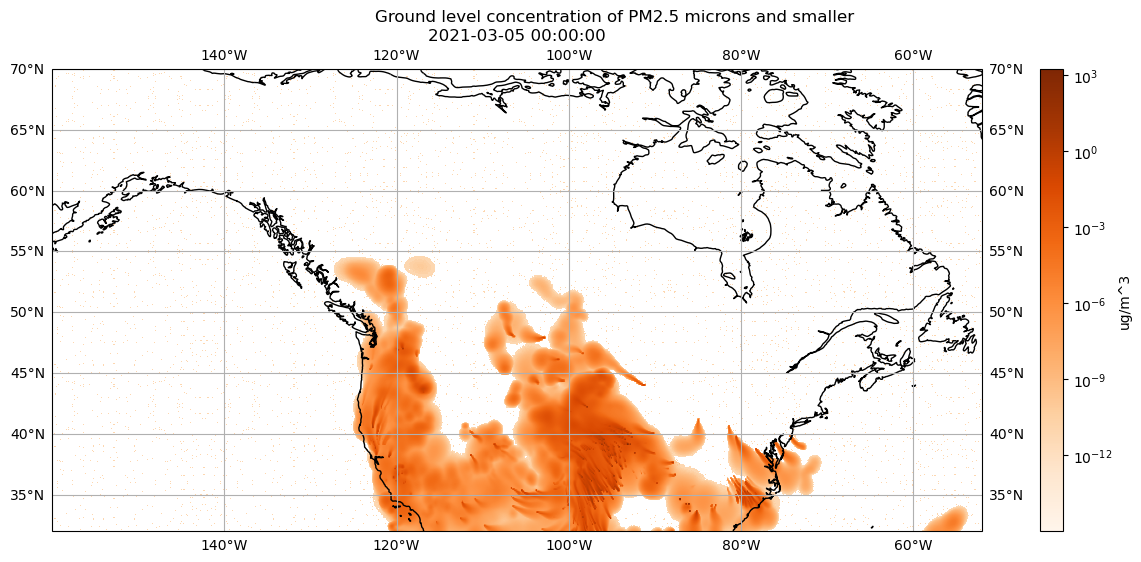
\includegraphics{demo_files/figure-latex/data_notebooks-demo-demo-cell-14-output-1.png}

Here we plot with xarray's built-in matplotlib powered plotter.

\begin{Shaded}
\begin{Highlighting}[]
\NormalTok{data\_array\_at\_time.plot(vmin}\OperatorTok{=}\DecValTok{0}\NormalTok{, vmax}\OperatorTok{=}\DecValTok{30}\NormalTok{)}
\end{Highlighting}
\end{Shaded}

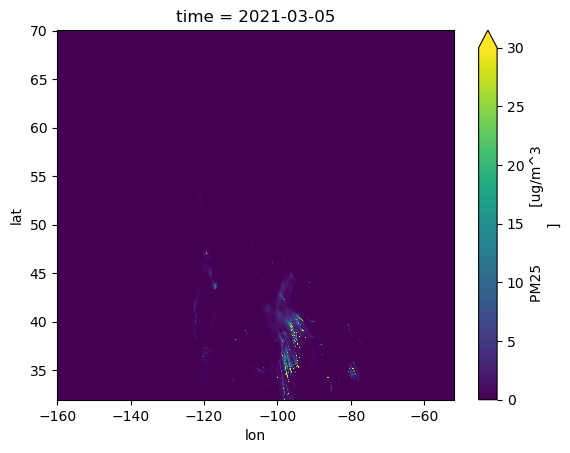
\includegraphics{demo_files/figure-latex/data_notebooks-demo-demo-cell-15-output-1.png}

Here we plot data\_array\_at\_latlon. We use the exact same code, but
define \texttt{my\_extent} accordingly.

\begin{Shaded}
\begin{Highlighting}[]
\CommentTok{\# Let\textquotesingle{}s use matplotlib\textquotesingle{}s imshow, since our data is on a grid}
\CommentTok{\# ref: https://matplotlib.org/stable/api/\_as\_gen/matplotlib.pyplot.imshow.html}

\CommentTok{\# Initialize a figure and plot, so we can customize figure and plot of data}
\CommentTok{\# ref: https://matplotlib.org/stable/api/\_as\_gen/matplotlib.pyplot.subplots.html}
\NormalTok{my\_fig, my\_plt }\OperatorTok{=}\NormalTok{ plt.subplots(figsize}\OperatorTok{=}\NormalTok{(}\DecValTok{15}\NormalTok{, }\DecValTok{6}\NormalTok{), subplot\_kw}\OperatorTok{=}\BuiltInTok{dict}\NormalTok{(projection}\OperatorTok{=}\NormalTok{ccrs.PlateCarree()))}

\CommentTok{\# Let\textquotesingle{}s set some parameters to get the visualization we want}
\CommentTok{\# ref: https://matplotlib.org/stable/api/\_as\_gen/matplotlib.pyplot.imshow.html}

\CommentTok{\# color PM25 values on a log scale, since values are small}
\NormalTok{my\_norm }\OperatorTok{=} \StringTok{"log"} 
\CommentTok{\# ***this will number our x and y axes based on the longitude latitude range***}
\NormalTok{my\_extent }\OperatorTok{=}\NormalTok{ [min\_lon, max\_lon, min\_lat, max\_lat]}
\CommentTok{\# ensure the aspect ratio of our plot fits all data, matplotlib can does this automatically}
\NormalTok{my\_aspect }\OperatorTok{=} \StringTok{\textquotesingle{}auto\textquotesingle{}}
\CommentTok{\# tell matplotlib, our origin is the lower{-}left corner}
\NormalTok{my\_origin }\OperatorTok{=} \StringTok{\textquotesingle{}lower\textquotesingle{}}
\CommentTok{\# select a colormap for our plot and the color bar on the right}
\NormalTok{my\_cmap }\OperatorTok{=} \StringTok{\textquotesingle{}Oranges\textquotesingle{}}

\CommentTok{\# create our plot using imshow}
\NormalTok{plot }\OperatorTok{=}\NormalTok{ plt.imshow(data\_array\_at\_latlon.values, norm}\OperatorTok{=}\NormalTok{my\_norm, extent}\OperatorTok{=}\NormalTok{my\_extent, }
\NormalTok{          aspect}\OperatorTok{=}\NormalTok{my\_aspect, origin}\OperatorTok{=}\NormalTok{my\_origin, cmap}\OperatorTok{=}\NormalTok{my\_cmap)}

\CommentTok{\# draw coastlines}
\NormalTok{my\_plt.coastlines()}

\CommentTok{\# draw latitude longitude lines}
\CommentTok{\# ref: https://scitools.org.uk/cartopy/docs/latest/gallery/gridlines\_and\_labels/gridliner.html}
\NormalTok{my\_plt.gridlines(draw\_labels}\OperatorTok{=}\VariableTok{True}\NormalTok{)}

\CommentTok{\# add a colorbar to our figure, based on the plot we just made above}
\NormalTok{my\_fig.colorbar(plot,location}\OperatorTok{=}\StringTok{\textquotesingle{}right\textquotesingle{}}\NormalTok{, label}\OperatorTok{=}\StringTok{\textquotesingle{}ug/m\^{}3\textquotesingle{}}\NormalTok{)}

\CommentTok{\# Add metadata as text annotations}
\NormalTok{metadata\_text }\OperatorTok{=}\NormalTok{ (}
    \SpecialStringTok{f\textquotesingle{}resampled: }\SpecialCharTok{\{}\NormalTok{resampled}\SpecialCharTok{.}\NormalTok{values}\SpecialCharTok{\}}\CharTok{\textbackslash{}n}\SpecialStringTok{\textquotesingle{}}
    \SpecialStringTok{f\textquotesingle{}SDATE: }\SpecialCharTok{\{}\NormalTok{sdate}\SpecialCharTok{.}\NormalTok{values}\SpecialCharTok{\}}\CharTok{\textbackslash{}n}\SpecialStringTok{\textquotesingle{}}
    \SpecialStringTok{f\textquotesingle{}STIME: }\SpecialCharTok{\{}\NormalTok{stime}\SpecialCharTok{.}\NormalTok{values}\SpecialCharTok{\}}\CharTok{\textbackslash{}n}\SpecialStringTok{\textquotesingle{}}
    \SpecialStringTok{f\textquotesingle{}WDATE: }\SpecialCharTok{\{}\NormalTok{wdate}\SpecialCharTok{.}\NormalTok{values}\SpecialCharTok{\}}\CharTok{\textbackslash{}n}\SpecialStringTok{\textquotesingle{}}
    \SpecialStringTok{f\textquotesingle{}WTIME: }\SpecialCharTok{\{}\NormalTok{wtime}\SpecialCharTok{.}\NormalTok{values}\SpecialCharTok{\}}\SpecialStringTok{\textquotesingle{}}
\NormalTok{)}

\CommentTok{\# Place metadata text on the plot}
\NormalTok{my\_plt.text(}\FloatTok{0.02}\NormalTok{, }\FloatTok{0.02}\NormalTok{, metadata\_text, transform}\OperatorTok{=}\NormalTok{my\_plt.transAxes,}
\NormalTok{            fontsize}\OperatorTok{=}\DecValTok{12}\NormalTok{, verticalalignment}\OperatorTok{=}\StringTok{\textquotesingle{}bottom\textquotesingle{}}\NormalTok{, bbox}\OperatorTok{=}\BuiltInTok{dict}\NormalTok{(facecolor}\OperatorTok{=}\StringTok{\textquotesingle{}white\textquotesingle{}}\NormalTok{, alpha}\OperatorTok{=}\FloatTok{0.8}\NormalTok{))}

\CommentTok{\# Set x and y axis labels on our ax}
\NormalTok{my\_fig.supxlabel(}\StringTok{\textquotesingle{}Longitude\textquotesingle{}}\NormalTok{)}
\NormalTok{my\_fig.supylabel(}\StringTok{\textquotesingle{}Latitude\textquotesingle{}}\NormalTok{)}

\CommentTok{\# Set title of our figure}
\NormalTok{my\_fig.suptitle(}\StringTok{\textquotesingle{}Ground level concentration of PM2.5 microns and smaller\textquotesingle{}}\NormalTok{)}

\CommentTok{\# Set title of our plot as the timestamp of our data}
\NormalTok{my\_plt.set\_title(}\SpecialStringTok{f\textquotesingle{}}\SpecialCharTok{\{}\NormalTok{my\_timestamp}\SpecialCharTok{\}}\SpecialStringTok{\textquotesingle{}}\NormalTok{)}

\CommentTok{\# Show the resulting visualization}
\NormalTok{plt.show()}
\end{Highlighting}
\end{Shaded}

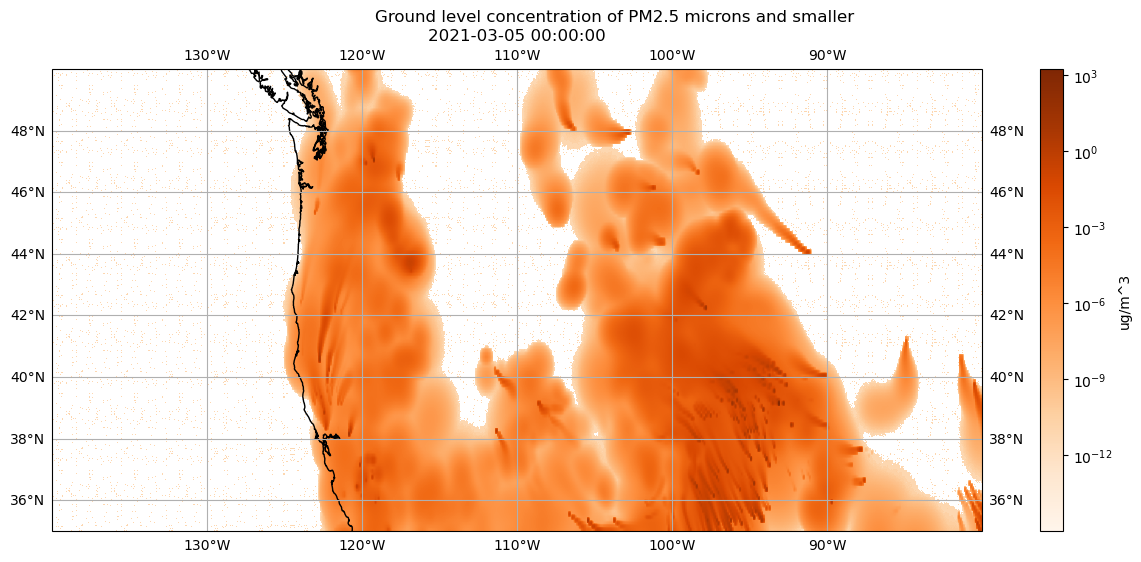
\includegraphics{demo_files/figure-latex/data_notebooks-demo-demo-cell-16-output-1.png}

\begin{Shaded}
\begin{Highlighting}[]
\NormalTok{data\_array\_at\_latlon.plot(vmin}\OperatorTok{=}\DecValTok{0}\NormalTok{, vmax}\OperatorTok{=}\DecValTok{30}\NormalTok{)}
\end{Highlighting}
\end{Shaded}

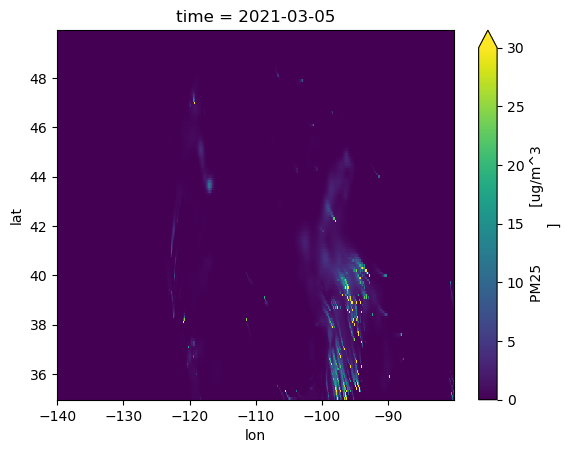
\includegraphics{demo_files/figure-latex/data_notebooks-demo-demo-cell-17-output-1.png}

\subsection{\texorpdfstring{\emph{Please reach out to Arleth Salinas or
Valerio Pascucci for any concerns about the notebook. Thank
you!}}{Please reach out to Arleth Salinas or Valerio Pascucci for any concerns about the notebook. Thank you!}}\label{please-reach-out-to-arleth-salinas-or-valerio-pascucci-for-any-concerns-about-the-notebook.-thank-you}

\begin{itemize}
\tightlist
\item
  Arleth Salinas (arleth.salinas@utah.edu)
\item
  Valerio Pascucci (pascucci.valerio@gmail.com)
\end{itemize}

\bookmarksetup{startatroot}

\chapter{Introduction}\label{sec-introduction}

Wildfires in North America have significantly impacted ecosystems and
human society {[}1{]}. Climate change affects the frequency, duration,
and severity of wildfires thus necessitating the use of wildfire
prediction systems to effectively mitigate wildfire impact. However,
data for understanding the impact of climate change on wildfires is
limited, only available for a few regions and for only a few decades
{[}2{]}. Furthermore, wildfire prediction systems in North America
prioritize decision making and fire management on short timescales, from
minutes to months. Therefore, long term wildfire prediction systems have
limited access to aggregate short term data, due to resource constraints
from fire management entities to share the data they collect and curate.

The Weather Forecast Research Team at the University of British Columbia
(UBC) generates a short term dataset of PM2.5 smoke particulate presence
in North America. Over the past 3 years, each day four times a day, UBC
has created forecasts of PM2.5 smoke particulate on the ground for
Canada and the continental United States. This is done using their The
BlueSky Western Canada Wildfire Smoke Forecasting System. UBC provides
access to this data to paying customers and for free on a daily basis
via a web-based visualization and file download.

These smoke predictions are useful for those who must make decisions on
how to deal with smoke as it comes. However, these years of forecasts
are not available in a non-trivial fashion for long term forecasting.
The data only exists among the hundreds of NetCDF files that UBC has
generated.

Our task is to obtain a single long term dataset from the smoke forecast
files that are available from UBC.

\bookmarksetup{startatroot}

\chapter{References}\label{references}

\bookmarksetup{startatroot}

\chapter{System and Environment}\label{sec-sys-specs}

\section{Machine Specification}\label{machine-specification}

The data we curate is over 300 gigabytes large. Therefore we used the
SCI institute's in-house machine `atlantis' for data staging and
processing. See Table~\ref{tbl-specs}.

\begin{longtable}[]{@{}ll@{}}
\caption{`atlantis' System
Specifications}\label{tbl-specs}\tabularnewline
\toprule\noalign{}
Property & Value \\
\midrule\noalign{}
\endfirsthead
\toprule\noalign{}
Property & Value \\
\midrule\noalign{}
\endhead
\bottomrule\noalign{}
\endlastfoot
Architecture & x86\_64 \\
CPU op-mode(s) & 32-bit, 64-bit \\
Byte Order & Little Endian \\
Address sizes & 44 bits physical, 48 bits virtual \\
CPU(s) & 48 \\
On-line CPU(s) list & 0-47 \\
Thread(s) per core & 2 \\
Core(s) per socket & 6 \\
Socket(s) & 4 \\
\end{longtable}

\section{Environment}\label{environment}

We aim to work in an environment that can be most easily reproduced and
documented. Therefore we used Python 3.9.19 via conda. We did all our
work within the Project Jupyter environment.

To find our the \texttt{yml} file containing our exported conda
environment please see the sidebar.

To work on the `atlantis' machine, we used SSH to connect to the
machine.

In the proceeding chapters we will specify which tools and libraries
were used and why.

\bookmarksetup{startatroot}

\chapter{The Data Source}\label{sec-data-source}

It is important to understand exactly what data is available and how to
obtain that data.

We encourage you to explore the dataset on
\href{https://firesmoke.ca/forecasts/}{UBC's website} to further
understand the dataset's use as described by UBC.

Here we establish:

\begin{itemize}
\tightlist
\item
  What systems are available to obtain the smoke forecast data from UBC?
\item
  What are in the files that UBC provides?
\item
  What metadata is associated with the files we obtain, both from within
  the file and about the files as a whole?
\end{itemize}

This information \textbf{was not} determined the first time we explored
this dataset.

As seen in the later chapters, we operated under misinformed assumptions
and encountered issues only resolvable by operating on the data
``blindly''. The purpose of this chapter is to establish the final set
of information we learned about our data source after extensive
exploration and manipulation.

\section{Overview}\label{overview}

The Weather Forecast Research Team at the University of British Columbia
(UBC) generates a short term dataset of PM2.5 smoke particulate presence
in North America. This is done using their
\href{https://firesmoke.ca/resources/bsc-2014-description.pdf}{The
BlueSky Western Canada Wildfire Smoke Forecasting System}. Over the past
3 years, each day four times a day, UBC creates 2-day forecasts of PM2.5
smoke particulate on the ground for Canada and the continental United
States. Each such forecast is downloadable as a NetCDF file or KMZ file.
UBC provides access to these predictions for free on a daily basis at
their website \href{https://firesmoke.ca/}{firesmoke.ca}.

\section{UBC Smoke Forecast Files
Access}\label{ubc-smoke-forecast-files-access}

\subsection{Available Forecasts}\label{available-forecasts}

All forecast files are uniquely identifiable with a forecast ID based on
when their meteorology forecast is initiated, a smoke forecast
initialization time, and by date. The time ranges of available files by
forecast ID is shown in Table~\ref{tbl-time}. Please note, there are
occassional \textbf{failed forecasts or otherwise unavailable files}
within the date ranges specified Table~\ref{tbl-time}, see
Section~\ref{sec-collection-info} for further details.

\begin{longtable}[]{@{}
  >{\raggedright\arraybackslash}p{(\columnwidth - 8\tabcolsep) * \real{0.1364}}
  >{\raggedright\arraybackslash}p{(\columnwidth - 8\tabcolsep) * \real{0.3000}}
  >{\raggedright\arraybackslash}p{(\columnwidth - 8\tabcolsep) * \real{0.3091}}
  >{\raggedright\arraybackslash}p{(\columnwidth - 8\tabcolsep) * \real{0.1273}}
  >{\raggedright\arraybackslash}p{(\columnwidth - 8\tabcolsep) * \real{0.1273}}@{}}
\caption{Dates for which all forecast ID datasets are publicly
available. All times are in UTC and the grid size is 12
km.}\label{tbl-time}\tabularnewline
\toprule\noalign{}
\begin{minipage}[b]{\linewidth}\raggedright
Forecast ID
\end{minipage} & \begin{minipage}[b]{\linewidth}\raggedright
Meteorology Forecast Initialization (UTC)
\end{minipage} & \begin{minipage}[b]{\linewidth}\raggedright
Smoke Forecast Initialization (UTC)
\end{minipage} & \begin{minipage}[b]{\linewidth}\raggedright
Start Date
\end{minipage} & \begin{minipage}[b]{\linewidth}\raggedright
End Date
\end{minipage} \\
\midrule\noalign{}
\endfirsthead
\toprule\noalign{}
\begin{minipage}[b]{\linewidth}\raggedright
Forecast ID
\end{minipage} & \begin{minipage}[b]{\linewidth}\raggedright
Meteorology Forecast Initialization (UTC)
\end{minipage} & \begin{minipage}[b]{\linewidth}\raggedright
Smoke Forecast Initialization (UTC)
\end{minipage} & \begin{minipage}[b]{\linewidth}\raggedright
Start Date
\end{minipage} & \begin{minipage}[b]{\linewidth}\raggedright
End Date
\end{minipage} \\
\midrule\noalign{}
\endhead
\bottomrule\noalign{}
\endlastfoot
BSC00CA12-01 & 00Z & 08Z & March 4, 2021 & Present Day \\
BSC06CA12-01 & 06Z & 14Z & March 4, 2021 & Present Day \\
BSC12CA12-01 & 12Z & 20Z & March 3, 2021 & Present Day \\
BSC18CA12-01 & 18Z & 02Z & March 4, 2021 & Present Day \\
\end{longtable}

The smoke forecasts are updated daily, including the present day, so
there is no fixed end date. Therefore, the latest data must be
downloaded on a regular basis. We have not implemented this process yet,
so the latest forecast files we use are up to June 27, 2024.

There is no official source stating the earliest available date for each
forecast. So, knowing the project began in 2021, we inferenced that the
earliest available date would be in 2021. Via trial and error we found
the earliest available dates.

\subsection{Download Instructions}\label{sec-download-instructions}

To download the 2-day forecast for the forecast initialization date of
one's choice, one follows the instructions below. The downloaded file
can be a NetCDF or KMZ file. Go to the URL:
\texttt{https://firesmoke.ca/forecasts/\{Forecast\ ID\}/\{YYYYMMDD\}\{InitTime\}/\{File\ Type\}}

Where:

\begin{itemize}
\tightlist
\item
  \texttt{YYYYMMDD} is the date of choice.
\item
  \texttt{ForecastID} and \texttt{InitTime} are the chosen values as
  described in Table~\ref{tbl-access}.
\item
  \texttt{File\ Type} is either \texttt{dispersion.nc} or
  \texttt{dispersion.kmz} for either the NetCDF file or KMZ file,
  respectively.
\end{itemize}

\begin{longtable}[]{@{}ll@{}}
\caption{UBC Smoke Forecast Data Download Parameters. All times are in
UTC and the grid size is 12 km.}\label{tbl-access}\tabularnewline
\toprule\noalign{}
Forecast ID & Smoke Forecast Initialization (UTC) \\
\midrule\noalign{}
\endfirsthead
\toprule\noalign{}
Forecast ID & Smoke Forecast Initialization (UTC) \\
\midrule\noalign{}
\endhead
\bottomrule\noalign{}
\endlastfoot
BSC00CA12-01 & 08Z \\
BSC06CA12-01 & 14Z \\
BSC12CA12-01 & 20Z \\
BSC18CA12-01 & 02Z \\
\end{longtable}

\subsubsection{Download Example}\label{download-example}

Let's try downloading the forecast for January 1, 2024 where the weather
forecast is initiated at 00:00:00 UTC and the smoke forecast is
initialized at 08:00:00 UTC by navigating to the corresponding URL.

\begin{Shaded}
\begin{Highlighting}[]
\NormalTok{forecast\_id }\OperatorTok{=} \StringTok{"BSC00CA12{-}01"}
\NormalTok{yyyymmdd }\OperatorTok{=} \StringTok{"20210304"}
\NormalTok{init\_time }\OperatorTok{=} \StringTok{"08"}

\NormalTok{url }\OperatorTok{=}\NormalTok{ (}
    \SpecialStringTok{f"https://firesmoke.ca/forecasts/}\SpecialCharTok{\{}\NormalTok{forecast\_id}\SpecialCharTok{\}}\SpecialStringTok{/}\SpecialCharTok{\{}\NormalTok{yyyymmdd}\SpecialCharTok{\}\{}\NormalTok{init\_time}\SpecialCharTok{\}}\SpecialStringTok{/dispersion.nc"}
\NormalTok{)}

\BuiltInTok{print}\NormalTok{(}\SpecialStringTok{f"Navigate to this URL in your browser: }\SpecialCharTok{\{}\NormalTok{url}\SpecialCharTok{\}}\SpecialStringTok{"}\NormalTok{)}
\end{Highlighting}
\end{Shaded}

\begin{verbatim}
Navigate to this URL in your browser: https://firesmoke.ca/forecasts/BSC00CA12-01/2021030408/dispersion.nc
\end{verbatim}

\section{The NetCDF File}\label{the-netcdf-file}

Next, let's look at what is within the NetCDF file located at the URL in
our previous example.

\subsection{File Preview}\label{file-preview}

We load \texttt{dispersion.nc} using \texttt{xarray}, which provides a
preview of the file.

\begin{Shaded}
\begin{Highlighting}[]
\ImportTok{import}\NormalTok{ xarray }\ImportTok{as}\NormalTok{ xr}

\NormalTok{ds }\OperatorTok{=}\NormalTok{ xr.open\_dataset(}\StringTok{"data\_notebooks/data\_source/dispersion.nc"}\NormalTok{)}
\NormalTok{ds}
\end{Highlighting}
\end{Shaded}

\begin{verbatim}
<xarray.Dataset>
Dimensions:  (TSTEP: 51, VAR: 1, DATE-TIME: 2, LAY: 1, ROW: 381, COL: 1041)
Dimensions without coordinates: TSTEP, VAR, DATE-TIME, LAY, ROW, COL
Data variables:
    TFLAG    (TSTEP, VAR, DATE-TIME) int32 ...
    PM25     (TSTEP, LAY, ROW, COL) float32 ...
Attributes: (12/33)
    IOAPI_VERSION:  $Id: @(#) ioapi library version 3.0 $                    ...
    EXEC_ID:        ????????????????                                         ...
    FTYPE:          1
    CDATE:          2021063
    CTIME:          101914
    WDATE:          2021063
    ...             ...
    VGLVLS:         [10.  0.]
    GDNAM:          HYSPLIT CONC    
    UPNAM:          hysplit2netCDF  
    VAR-LIST:       PM25            
    FILEDESC:       Hysplit Concentration Model Output                       ...
    HISTORY:        
\end{verbatim}

\subsection{File Attributes}\label{file-attributes}

\texttt{dispersion.nc} contains the following attributes. Note that for
all files across forecast IDs, they have the same dimension and variable
names:

\subsubsection{Dimensions:}\label{dimensions}

The dimensions described in Table~\ref{tbl-dims} determine on which
indicies we may index our variables.

\begin{longtable}[]{@{}
  >{\raggedright\arraybackslash}p{(\columnwidth - 4\tabcolsep) * \real{0.1026}}
  >{\raggedright\arraybackslash}p{(\columnwidth - 4\tabcolsep) * \real{0.0513}}
  >{\raggedright\arraybackslash}p{(\columnwidth - 4\tabcolsep) * \real{0.8462}}@{}}
\caption{Description of Dimensions for Indexing Data in NetCDF
Files}\label{tbl-dims}\tabularnewline
\toprule\noalign{}
\begin{minipage}[b]{\linewidth}\raggedright
Dimension
\end{minipage} & \begin{minipage}[b]{\linewidth}\raggedright
Size
\end{minipage} & \begin{minipage}[b]{\linewidth}\raggedright
Description
\end{minipage} \\
\midrule\noalign{}
\endfirsthead
\toprule\noalign{}
\begin{minipage}[b]{\linewidth}\raggedright
Dimension
\end{minipage} & \begin{minipage}[b]{\linewidth}\raggedright
Size
\end{minipage} & \begin{minipage}[b]{\linewidth}\raggedright
Description
\end{minipage} \\
\midrule\noalign{}
\endhead
\bottomrule\noalign{}
\endlastfoot
TSTEP & 51 & This dimension represents the number of time steps in the
file. Each file has 51 hours represented. \\
VAR & 1 & This dimension is a placeholder for the variables in the
file. \\
DATE-TIME & 2 & This dimension stores the date and time information for
each time step. \\
LAY & 1 & This dimension represents the number of layers in the file,
which is 1 in this case. \\
ROW & 381 & This dimension represents the number of rows in the spatial
grid. \\
COL & 1041 & This dimension represents the number of columns in the
spatial grid. \\
\end{longtable}

\subsubsection{Variables:}\label{variables}

The variables described in Table~\ref{tbl-vars} contain the data in
question that we would like to extract.

\begin{longtable}[]{@{}
  >{\raggedright\arraybackslash}p{(\columnwidth - 6\tabcolsep) * \real{0.0758}}
  >{\raggedright\arraybackslash}p{(\columnwidth - 6\tabcolsep) * \real{0.1742}}
  >{\raggedright\arraybackslash}p{(\columnwidth - 6\tabcolsep) * \real{0.0833}}
  >{\raggedright\arraybackslash}p{(\columnwidth - 6\tabcolsep) * \real{0.6667}}@{}}
\caption{Description of Variables in NetCDF
Files}\label{tbl-vars}\tabularnewline
\toprule\noalign{}
\begin{minipage}[b]{\linewidth}\raggedright
Variable
\end{minipage} & \begin{minipage}[b]{\linewidth}\raggedright
Dimensions
\end{minipage} & \begin{minipage}[b]{\linewidth}\raggedright
Data Type
\end{minipage} & \begin{minipage}[b]{\linewidth}\raggedright
Description
\end{minipage} \\
\midrule\noalign{}
\endfirsthead
\toprule\noalign{}
\begin{minipage}[b]{\linewidth}\raggedright
Variable
\end{minipage} & \begin{minipage}[b]{\linewidth}\raggedright
Dimensions
\end{minipage} & \begin{minipage}[b]{\linewidth}\raggedright
Data Type
\end{minipage} & \begin{minipage}[b]{\linewidth}\raggedright
Description
\end{minipage} \\
\midrule\noalign{}
\endhead
\bottomrule\noalign{}
\endlastfoot
TFLAG & TSTEP, VAR, DATE-TIME & int32 & This variable stores the date
and time of each time step. \\
PM25 & TSTEP, LAY, ROW, COL & float32 & This variable contains the
concentration of particulate matter (PM2.5) for each time step, layer,
row, and column in the spatial grid. \\
\end{longtable}

\subsubsection{Attributes}\label{attributes}

Of the 33 available attributes we use the ones shown in
Table~\ref{tbl-attrs}:

\begin{longtable}[]{@{}
  >{\raggedright\arraybackslash}p{(\columnwidth - 4\tabcolsep) * \real{0.0797}}
  >{\raggedright\arraybackslash}p{(\columnwidth - 4\tabcolsep) * \real{0.1522}}
  >{\raggedright\arraybackslash}p{(\columnwidth - 4\tabcolsep) * \real{0.7681}}@{}}
\caption{Description of Attributes in NetCDF
Files}\label{tbl-attrs}\tabularnewline
\toprule\noalign{}
\begin{minipage}[b]{\linewidth}\raggedright
Attribute
\end{minipage} & \begin{minipage}[b]{\linewidth}\raggedright
Value
\end{minipage} & \begin{minipage}[b]{\linewidth}\raggedright
Description
\end{minipage} \\
\midrule\noalign{}
\endfirsthead
\toprule\noalign{}
\begin{minipage}[b]{\linewidth}\raggedright
Attribute
\end{minipage} & \begin{minipage}[b]{\linewidth}\raggedright
Value
\end{minipage} & \begin{minipage}[b]{\linewidth}\raggedright
Description
\end{minipage} \\
\midrule\noalign{}
\endhead
\bottomrule\noalign{}
\endlastfoot
CDATE & 2021063 & The creation date of the dataset, in YYYYDDD
format. \\
CTIME & 101914 & The creation time of the dataset, in HHMMSS format. \\
WDATE & 2021063 & The date for which the weather forecast is initiated,
in YYYYDDD format. \\
WTIME & 101914 & The time for which the weather forecast is initiated,
in HHMMSS format. \\
SDATE & 2021063 & The date for which the smoke forecast is initiated,in
YYYYDDD format. \\
STIME & 90000 & The time for which the weather forecast is initiated, in
HHMMSS format. \\
NCOLS & 1041 & The number of columns in the spatial grid. \\
NROWS & 381 & The number of rows in the spatial grid. \\
XORIG & -156.0 & The origin (starting point) of the grid in the
x-direction. \\
YORIG & 32.0 & The origin (starting point) of the grid in the
y-direction. \\
XCELL & 0.10000000149011612 & The cell size in the x-direction. \\
YCELL & 0.10000000149011612 & The cell size in the y-direction. \\
\end{longtable}

Let's look closer at what exactly is within one NetCDF file in the
following demo.

\subsection{NetCDF Visualization Demo}\label{sec-netcdf-demo}

In this demo we load one \texttt{dispersion.nc} file and explore how to
visualize the data within the file.

\subsubsection{Accessing the File}\label{accessing-the-file}

We use the forecast for March 4, 2021 where the weather forecast is
initiated at 00:00:00 UTC and the smoke forecast is initialized at
08:00:00 UTC. You can download this file by navigating to the URL below.

\begin{Shaded}
\begin{Highlighting}[]
\NormalTok{forecast\_id }\OperatorTok{=} \StringTok{"BSC00CA12{-}01"}
\NormalTok{yyyymmdd }\OperatorTok{=} \StringTok{"20210304"}
\NormalTok{init\_time }\OperatorTok{=} \StringTok{"08"}

\NormalTok{url }\OperatorTok{=}\NormalTok{ (}
    \SpecialStringTok{f"https://firesmoke.ca/forecasts/}\SpecialCharTok{\{}\NormalTok{forecast\_id}\SpecialCharTok{\}}\SpecialStringTok{/}\SpecialCharTok{\{}\NormalTok{yyyymmdd}\SpecialCharTok{\}\{}\NormalTok{init\_time}\SpecialCharTok{\}}\SpecialStringTok{/dispersion.nc"}
\NormalTok{)}

\BuiltInTok{print}\NormalTok{(}\SpecialStringTok{f"Download this file from URL: }\SpecialCharTok{\{}\NormalTok{url}\SpecialCharTok{\}}\SpecialStringTok{"}\NormalTok{)}

\ImportTok{import}\NormalTok{ urllib.request}
\NormalTok{urllib.request.urlretrieve(url, }\StringTok{"dispersion.nc"}\NormalTok{)}
\end{Highlighting}
\end{Shaded}

\begin{verbatim}
Download this file from URL: https://firesmoke.ca/forecasts/BSC00CA12-01/2021030408/dispersion.nc
\end{verbatim}

\paragraph{Opening the File}\label{opening-the-file}

We use xarray to open the NetCDF file and preview it.

\begin{Shaded}
\begin{Highlighting}[]
\ImportTok{import}\NormalTok{ xarray }\ImportTok{as}\NormalTok{ xr}

\NormalTok{ds }\OperatorTok{=}\NormalTok{ xr.open\_dataset(}\StringTok{"dispersion.nc"}\NormalTok{)}

\NormalTok{ds}
\end{Highlighting}
\end{Shaded}

\begin{verbatim}
<xarray.Dataset>
Dimensions:  (TSTEP: 51, VAR: 1, DATE-TIME: 2, LAY: 1, ROW: 381, COL: 1041)
Dimensions without coordinates: TSTEP, VAR, DATE-TIME, LAY, ROW, COL
Data variables:
    TFLAG    (TSTEP, VAR, DATE-TIME) int32 ...
    PM25     (TSTEP, LAY, ROW, COL) float32 ...
Attributes: (12/33)
    IOAPI_VERSION:  $Id: @(#) ioapi library version 3.0 $                    ...
    EXEC_ID:        ????????????????                                         ...
    FTYPE:          1
    CDATE:          2021063
    CTIME:          101914
    WDATE:          2021063
    ...             ...
    VGLVLS:         [10.  0.]
    GDNAM:          HYSPLIT CONC    
    UPNAM:          hysplit2netCDF  
    VAR-LIST:       PM25            
    FILEDESC:       Hysplit Concentration Model Output                       ...
    HISTORY:        
\end{verbatim}

\subsubsection{Using the Data}\label{using-the-data}

\paragraph{Accessing Arrays}\label{accessing-arrays}

The data we are interested in is the PM2.5 values. Let's use
\texttt{xarray} to preview the \texttt{PM25} variable in our file.

\begin{Shaded}
\begin{Highlighting}[]
\NormalTok{ds[}\StringTok{"PM25"}\NormalTok{]}
\end{Highlighting}
\end{Shaded}

\begin{verbatim}
<xarray.DataArray 'PM25' (TSTEP: 51, LAY: 1, ROW: 381, COL: 1041)>
[20227671 values with dtype=float32]
Dimensions without coordinates: TSTEP, LAY, ROW, COL
Attributes:
    long_name:  PM25            
    units:      ug/m^3          
    var_desc:   PM25                                                         ...
\end{verbatim}

The dimensions of the \texttt{PM25} data array are composed of
\texttt{TSTEP}, \texttt{LAY}, \texttt{ROW}, and \texttt{COL}. We do not
need the \texttt{LAY} dimension, so let's use \texttt{numpy} to remove
it.

\phantomsection\label{annotated-cell-47}%
\begin{Shaded}
\begin{Highlighting}[]
\ImportTok{import}\NormalTok{ numpy }\ImportTok{as}\NormalTok{ np}

\NormalTok{ds\_pm25\_vals }\OperatorTok{=}\NormalTok{ ds[}\StringTok{"PM25"}\NormalTok{].values }\hspace*{\fill}\NormalTok{\circled{1}}
\BuiltInTok{print}\NormalTok{(}\SpecialStringTok{f\textquotesingle{}The shape of the data contained in our files is: }\SpecialCharTok{\{}\NormalTok{np}\SpecialCharTok{.}\NormalTok{shape(ds\_pm25\_vals)}\SpecialCharTok{\}}\SpecialStringTok{\textquotesingle{}}\NormalTok{)}

\NormalTok{ds\_pm25\_vals }\OperatorTok{=}\NormalTok{ np.squeeze(ds\_pm25\_vals) }\hspace*{\fill}\NormalTok{\circled{2}}
\BuiltInTok{print}\NormalTok{(}\SpecialStringTok{f\textquotesingle{}After squeezing, the shape is: }\SpecialCharTok{\{}\NormalTok{np}\SpecialCharTok{.}\NormalTok{shape(ds\_pm25\_vals)}\SpecialCharTok{\}}\SpecialStringTok{\textquotesingle{}}\NormalTok{)}
\end{Highlighting}
\end{Shaded}

\begin{description}
\tightlist
\item[\circled{1}]
Use .values to get the four dimensional array.
\item[\circled{2}]
Use \texttt{np.squeeze} to drop the LAY axis
\end{description}

\begin{verbatim}
The shape of the data contained in our files is: (51, 1, 381, 1041)
After squeezing, the shape is: (51, 381, 1041)
\end{verbatim}

\paragraph{\texorpdfstring{Visualize Array in
\texttt{matplotlib}}{Visualize Array in matplotlib}}\label{visualize-array-in-matplotlib}

Now that we squeezed away the \texttt{LAY} dimension, we can index time
step 10 and use \texttt{matplotlib} to visualize the timestep

\phantomsection\label{annotated-cell-48}%
\begin{Shaded}
\begin{Highlighting}[]
\ImportTok{import}\NormalTok{ matplotlib.pyplot }\ImportTok{as}\NormalTok{ plt}

\NormalTok{tstep }\OperatorTok{=} \DecValTok{10}
\NormalTok{smoke\_at\_tstep }\OperatorTok{=}\NormalTok{ ds\_pm25\_vals[tstep, :, :]}

\NormalTok{my\_fig, my\_plt }\OperatorTok{=}\NormalTok{ plt.subplots(figsize}\OperatorTok{=}\NormalTok{(}\DecValTok{15}\NormalTok{, }\DecValTok{6}\NormalTok{))}

\NormalTok{my\_norm }\OperatorTok{=} \StringTok{"log"} \hspace*{\fill}\NormalTok{\circled{1}}
\NormalTok{my\_aspect }\OperatorTok{=} \StringTok{\textquotesingle{}auto\textquotesingle{}} \hspace*{\fill}\NormalTok{\circled{2}}
\NormalTok{my\_origin }\OperatorTok{=} \StringTok{\textquotesingle{}lower\textquotesingle{}} \hspace*{\fill}\NormalTok{\circled{3}}
\NormalTok{my\_cmap }\OperatorTok{=} \StringTok{\textquotesingle{}viridis\textquotesingle{}} \hspace*{\fill}\NormalTok{\circled{4}}
 
\NormalTok{plot }\OperatorTok{=}\NormalTok{ my\_plt.imshow(smoke\_at\_tstep, norm}\OperatorTok{=}\NormalTok{my\_norm, aspect}\OperatorTok{=}\NormalTok{my\_aspect, origin}\OperatorTok{=}\NormalTok{my\_origin, cmap}\OperatorTok{=}\NormalTok{my\_cmap) }\hspace*{\fill}\NormalTok{\circled{5}}

\NormalTok{my\_fig.colorbar(plot, location}\OperatorTok{=}\StringTok{\textquotesingle{}right\textquotesingle{}}\NormalTok{, label}\OperatorTok{=}\StringTok{\textquotesingle{}ug/m\^{}3\textquotesingle{}}\NormalTok{) }\hspace*{\fill}\NormalTok{\circled{6}}

\NormalTok{my\_fig.suptitle(}\StringTok{\textquotesingle{}Ground level concentration of PM2.5 microns and smaller\textquotesingle{}}\NormalTok{) }\hspace*{\fill}\NormalTok{\circled{7}}

\NormalTok{my\_plt.set\_title(}\SpecialStringTok{f\textquotesingle{}Timestep }\SpecialCharTok{\{}\NormalTok{tstep}\SpecialCharTok{\}}\SpecialStringTok{\textquotesingle{}}\NormalTok{) }\hspace*{\fill}\NormalTok{\circled{8}}

\NormalTok{plt.show() }\hspace*{\fill}\NormalTok{\circled{9}}
\end{Highlighting}
\end{Shaded}

\begin{description}
\tightlist
\item[\circled{1}]
Color PM25 values on a log scale, since values are small.
\item[\circled{2}]
Ensure the aspect ratio of our plot fits all data, \texttt{matplotlib}
can do this automatically.
\item[\circled{3}]
Tell \texttt{matplotlib} our origin is the lower-left corner.
\item[\circled{4}]
Select a colormap for our plot and draw the color bar on the right.
\item[\circled{5}]
Create our plot using \texttt{imshow}.
\item[\circled{6}]
Add a colorbar to our figure, based on the plot we just made above.
\item[\circled{7}]
Set title of our figure.
\item[\circled{8}]
Set title of our plot as the timestamp of our data.
\item[\circled{9}]
Show the resulting visualization.
\end{description}

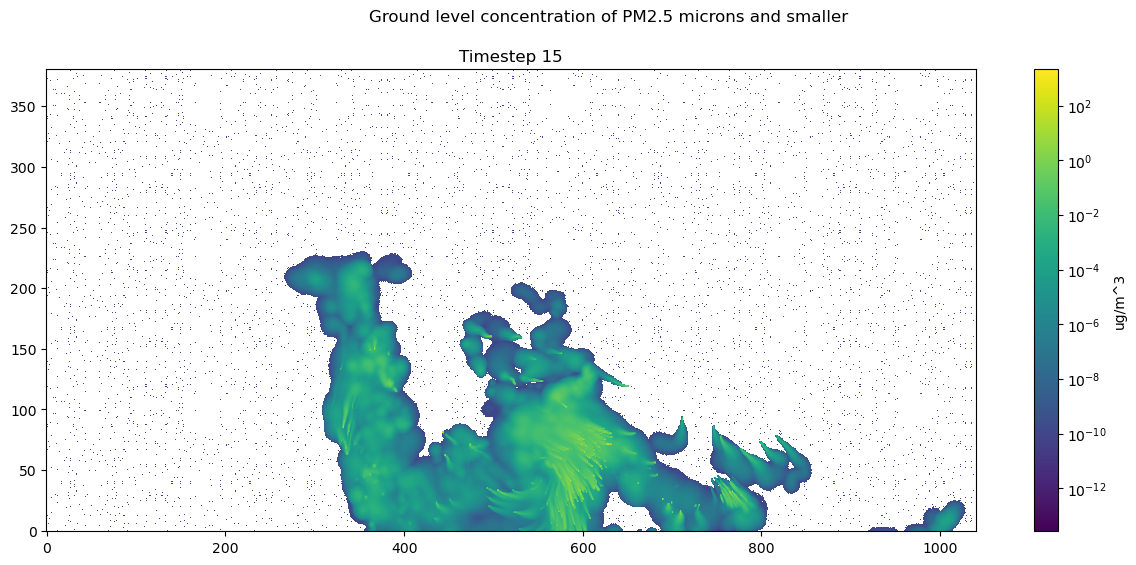
\includegraphics{data_source_files/figure-latex/data_notebooks-data_source-netcdf_demo-cell-6-output-1.png}

Notice there are no axis labels or metadata presented here. Next we will
show how to use the metadata in \texttt{dispersion.nc} so the data is
actually interpretable.

\subsubsection{Incorporating Metadata to Visualization via
Coordinates}\label{incorporating-metadata-to-visualization-via-coordinates}

\subparagraph{Latitude and Longitude
Coordinates}\label{latitude-and-longitude-coordinates}

\texttt{dispersion.nc} includes attributes to generate the latitude and
longitude values on the grid defined by \texttt{NCOLS} and
\texttt{NROWS}. We use this grid to match each data point in the
\texttt{PM25} variable to a lat/lon coordinate.

\begin{Shaded}
\begin{Highlighting}[]
\NormalTok{xorig }\OperatorTok{=}\NormalTok{ ds.XORIG}
\NormalTok{yorig }\OperatorTok{=}\NormalTok{ ds.YORIG}
\NormalTok{xcell }\OperatorTok{=}\NormalTok{ ds.XCELL}
\NormalTok{ycell }\OperatorTok{=}\NormalTok{ ds.YCELL}
\NormalTok{ncols }\OperatorTok{=}\NormalTok{ ds.NCOLS}
\NormalTok{nrows }\OperatorTok{=}\NormalTok{ ds.NROWS}

\NormalTok{longitude }\OperatorTok{=}\NormalTok{ np.linspace(xorig, xorig }\OperatorTok{+}\NormalTok{ xcell }\OperatorTok{*}\NormalTok{ (ncols }\OperatorTok{{-}} \DecValTok{1}\NormalTok{), ncols)}
\NormalTok{latitude }\OperatorTok{=}\NormalTok{ np.linspace(yorig, yorig }\OperatorTok{+}\NormalTok{ ycell }\OperatorTok{*}\NormalTok{ (nrows }\OperatorTok{{-}} \DecValTok{1}\NormalTok{), nrows)}

\BuiltInTok{print}\NormalTok{(}\StringTok{"Size of longitude \& latitude arrays:"}\NormalTok{)}
\BuiltInTok{print}\NormalTok{(}\SpecialStringTok{f\textquotesingle{}np.size(longitude) = }\SpecialCharTok{\{}\NormalTok{np}\SpecialCharTok{.}\NormalTok{size(longitude)}\SpecialCharTok{\}}\SpecialStringTok{\textquotesingle{}}\NormalTok{)}
\BuiltInTok{print}\NormalTok{(}\SpecialStringTok{f\textquotesingle{}np.size(latitude) = }\SpecialCharTok{\{}\NormalTok{np}\SpecialCharTok{.}\NormalTok{size(latitude)}\SpecialCharTok{\}}\CharTok{\textbackslash{}n}\SpecialStringTok{\textquotesingle{}}\NormalTok{)}
\BuiltInTok{print}\NormalTok{(}\StringTok{"Min \& Max of longitude and latitude arrays:"}\NormalTok{)}
\BuiltInTok{print}\NormalTok{(}\SpecialStringTok{f\textquotesingle{}longitude: min = }\SpecialCharTok{\{}\NormalTok{np}\SpecialCharTok{.}\BuiltInTok{min}\NormalTok{(longitude)}\SpecialCharTok{\}}\SpecialStringTok{, max = }\SpecialCharTok{\{}\NormalTok{np}\SpecialCharTok{.}\BuiltInTok{max}\NormalTok{(longitude)}\SpecialCharTok{\}}\SpecialStringTok{\textquotesingle{}}\NormalTok{)}
\BuiltInTok{print}\NormalTok{(}\SpecialStringTok{f\textquotesingle{}latitude: min = }\SpecialCharTok{\{}\NormalTok{np}\SpecialCharTok{.}\BuiltInTok{min}\NormalTok{(latitude)}\SpecialCharTok{\}}\SpecialStringTok{, max = }\SpecialCharTok{\{}\NormalTok{np}\SpecialCharTok{.}\BuiltInTok{max}\NormalTok{(latitude)}\SpecialCharTok{\}}\SpecialStringTok{\textquotesingle{}}\NormalTok{)}
\end{Highlighting}
\end{Shaded}

\begin{verbatim}
Size of longitude & latitude arrays:
np.size(longitude) = 1041
np.size(latitude) = 381

Min & Max of longitude and latitude arrays:
longitude: min = -156.0, max = -51.999998450279236
latitude: min = 32.0, max = 70.00000056624413
\end{verbatim}

\texttt{xarray} allows us to create coordinates, which maps variable
values to a value of our choice. In this case, we create coordinates
mapping PM25 values to a latitude and longitude value.

\phantomsection\label{annotated-cell-50}%
\begin{Shaded}
\begin{Highlighting}[]
\NormalTok{ds.coords[}\StringTok{\textquotesingle{}lat\textquotesingle{}}\NormalTok{] }\OperatorTok{=}\NormalTok{ (}\StringTok{\textquotesingle{}ROW\textquotesingle{}}\NormalTok{, latitude) }\hspace*{\fill}\NormalTok{\circled{1}}
\NormalTok{ds.coords[}\StringTok{\textquotesingle{}lon\textquotesingle{}}\NormalTok{] }\OperatorTok{=}\NormalTok{ (}\StringTok{\textquotesingle{}COL\textquotesingle{}}\NormalTok{, longitude)}

\NormalTok{ds }\OperatorTok{=}\NormalTok{ ds.swap\_dims(\{}\StringTok{\textquotesingle{}COL\textquotesingle{}}\NormalTok{: }\StringTok{\textquotesingle{}lon\textquotesingle{}}\NormalTok{, }\StringTok{\textquotesingle{}ROW\textquotesingle{}}\NormalTok{: }\StringTok{\textquotesingle{}lat\textquotesingle{}}\NormalTok{\}) }\hspace*{\fill}\NormalTok{\circled{2}}

\NormalTok{ds}
\end{Highlighting}
\end{Shaded}

\begin{description}
\tightlist
\item[\circled{1}]
Create coordinates for latitude and longitude.
\item[\circled{2}]
Replace \texttt{COL} and \texttt{ROW} dimensions with newly calculated
longitude and latitude coordinates.
\end{description}

\begin{verbatim}
<xarray.Dataset>
Dimensions:  (TSTEP: 51, VAR: 1, DATE-TIME: 2, LAY: 1, lat: 381, lon: 1041)
Coordinates:
  * lat      (lat) float64 32.0 32.1 32.2 32.3 32.4 ... 69.6 69.7 69.8 69.9 70.0
  * lon      (lon) float64 -156.0 -155.9 -155.8 -155.7 ... -52.2 -52.1 -52.0
Dimensions without coordinates: TSTEP, VAR, DATE-TIME, LAY
Data variables:
    TFLAG    (TSTEP, VAR, DATE-TIME) int32 ...
    PM25     (TSTEP, LAY, lat, lon) float32 0.0 0.0 0.0 0.0 ... 0.0 0.0 0.0 0.0
Attributes: (12/33)
    IOAPI_VERSION:  $Id: @(#) ioapi library version 3.0 $                    ...
    EXEC_ID:        ????????????????                                         ...
    FTYPE:          1
    CDATE:          2021063
    CTIME:          101914
    WDATE:          2021063
    ...             ...
    VGLVLS:         [10.  0.]
    GDNAM:          HYSPLIT CONC    
    UPNAM:          hysplit2netCDF  
    VAR-LIST:       PM25            
    FILEDESC:       Hysplit Concentration Model Output                       ...
    HISTORY:        
\end{verbatim}

Now let's move on to incorporating time stamp metadata.

\paragraph{Time Coordinates}\label{time-coordinates}

Recall, there is a \texttt{TFLAG} variable in \texttt{dispersion.nc}.

\begin{Shaded}
\begin{Highlighting}[]
\NormalTok{ds[}\StringTok{\textquotesingle{}TFLAG\textquotesingle{}}\NormalTok{]}
\end{Highlighting}
\end{Shaded}

\begin{verbatim}
<xarray.DataArray 'TFLAG' (TSTEP: 51, VAR: 1, DATE-TIME: 2)>
[102 values with dtype=int32]
Dimensions without coordinates: TSTEP, VAR, DATE-TIME
Attributes:
    units:      <YYYYDDD,HHMMSS>
    long_name:  TFLAG           
    var_desc:   Timestep-valid flags:  (1) YYYYDDD or (2) HHMMSS             ...
\end{verbatim}

The earliest and latest \texttt{TFLAG}s look like the following:

\begin{Shaded}
\begin{Highlighting}[]
\BuiltInTok{print}\NormalTok{(}\SpecialStringTok{f"Earliest available TFLAG is }\SpecialCharTok{\{}\NormalTok{ds[}\StringTok{\textquotesingle{}TFLAG\textquotesingle{}}\NormalTok{]}\SpecialCharTok{.}\NormalTok{values[}\DecValTok{0}\NormalTok{][}\DecValTok{0}\NormalTok{]}\SpecialCharTok{\}}\SpecialStringTok{"}\NormalTok{)}
\BuiltInTok{print}\NormalTok{(}\SpecialStringTok{f"Latest available TFLAG is }\SpecialCharTok{\{}\NormalTok{ds[}\StringTok{\textquotesingle{}TFLAG\textquotesingle{}}\NormalTok{]}\SpecialCharTok{.}\NormalTok{values[}\OperatorTok{{-}}\DecValTok{1}\NormalTok{][}\DecValTok{0}\NormalTok{]}\SpecialCharTok{\}}\SpecialStringTok{"}\NormalTok{)}
\end{Highlighting}
\end{Shaded}

\begin{verbatim}
Earliest available TFLAG is [2021063   90000]
Latest available TFLAG is [0 0]
\end{verbatim}

This time flags require processing to be immediately legible. Let's
write a function to process the time flag accordingly. We use the
\texttt{datetime} library.

\phantomsection\label{annotated-cell-53}%
\begin{Shaded}
\begin{Highlighting}[]
\ImportTok{import}\NormalTok{ datetime}

\KeywordTok{def}\NormalTok{ parse\_tflag(tflag):}
    \CommentTok{"""}
\CommentTok{    Return the tflag as a datetime object}
\CommentTok{    :param list tflag: a list of two int32, the 1st representing date and 2nd representing time}
\CommentTok{    """}
\NormalTok{    date }\OperatorTok{=} \BuiltInTok{int}\NormalTok{(tflag[}\DecValTok{0}\NormalTok{]) }\hspace*{\fill}\NormalTok{\circled{1}}
\NormalTok{    year }\OperatorTok{=}\NormalTok{ date }\OperatorTok{//} \DecValTok{1000} \hspace*{\fill}\NormalTok{\circled{2}}
\NormalTok{    day\_of\_year }\OperatorTok{=}\NormalTok{ date }\OperatorTok{\%} \DecValTok{1000} \hspace*{\fill}\NormalTok{\circled{3}}

\NormalTok{    final\_date }\OperatorTok{=}\NormalTok{ datetime.datetime(year, }\DecValTok{1}\NormalTok{, }\DecValTok{1}\NormalTok{) }\OperatorTok{+}\NormalTok{ datetime.timedelta(days}\OperatorTok{=}\NormalTok{day\_of\_year }\OperatorTok{{-}} \DecValTok{1}\NormalTok{) }\hspace*{\fill}\NormalTok{\circled{4}}

\NormalTok{    time }\OperatorTok{=} \BuiltInTok{int}\NormalTok{(tflag[}\DecValTok{1}\NormalTok{]) }\hspace*{\fill}\NormalTok{\circled{5}}
\NormalTok{    hours }\OperatorTok{=}\NormalTok{ time }\OperatorTok{//} \DecValTok{10000} \hspace*{\fill}\NormalTok{\circled{6}}
\NormalTok{    minutes }\OperatorTok{=}\NormalTok{ (time }\OperatorTok{\%} \DecValTok{10000}\NormalTok{) }\OperatorTok{//} \DecValTok{100} \hspace*{\fill}\NormalTok{\circled{7}}
\NormalTok{    seconds }\OperatorTok{=}\NormalTok{ time }\OperatorTok{\%} \DecValTok{100} \hspace*{\fill}\NormalTok{\circled{8}}

\NormalTok{    full\_datetime }\OperatorTok{=}\NormalTok{ datetime.datetime(year, final\_date.month, final\_date.day, hours, minutes, seconds) }\hspace*{\fill}\NormalTok{\circled{9}}
    \ControlFlowTok{return}\NormalTok{ full\_datetime}
\end{Highlighting}
\end{Shaded}

\begin{description}
\tightlist
\item[\circled{1}]
Obtain year and day of year from \texttt{tflag{[}0{]}} (date).
\item[\circled{2}]
Extract the year from the first 4 digits of \texttt{tflag{[}0{]}}.
\item[\circled{3}]
Extract the day of the year from the last 3 digits of
\texttt{tflag{[}0{]}}.
\item[\circled{4}]
Create a \texttt{datetime} object representing the date.
\item[\circled{5}]
Obtain hour, minutes, and seconds from \texttt{tflag{[}1{]}} (time).
\item[\circled{6}]
Extract hours from the first 2 digits of \texttt{tflag{[}1{]}}.
\item[\circled{7}]
Extract minutes from the 3rd and 4th digits of \texttt{tflag{[}1{]}}.
\item[\circled{8}]
Extract seconds from the last 2 digits of \texttt{tflag{[}1{]}}.
\item[\circled{9}]
Create the final \texttt{datetime} object with the extracted date and
time components.
\end{description}

Now we have datetime objects to represent the timeflag in a more legible
and usable format.

\begin{Shaded}
\begin{Highlighting}[]
\BuiltInTok{print}\NormalTok{(}\SpecialStringTok{f"Earliest available TFLAG is }\SpecialCharTok{\{}\NormalTok{parse\_tflag(ds[}\StringTok{\textquotesingle{}TFLAG\textquotesingle{}}\NormalTok{].values[}\DecValTok{0}\NormalTok{][}\DecValTok{0}\NormalTok{])}\SpecialCharTok{\}}\SpecialStringTok{"}\NormalTok{)}
\CommentTok{\# print(f"Latest available TFLAG is \{parse\_tflag(ds[\textquotesingle{}TFLAG\textquotesingle{}].values[{-}1][0])\}")}
\end{Highlighting}
\end{Shaded}

\begin{verbatim}
Earliest available TFLAG is 2021-03-04 09:00:00
\end{verbatim}

\paragraph{\texorpdfstring{Visualize Array in
\texttt{matplotlib}}{Visualize Array in matplotlib}}\label{visualize-array-in-matplotlib-1}

Let's visualize timestep 10 again, but now we can label the data using
latitudes and longitudes, and the corresponding time flag.

\phantomsection\label{annotated-cell-55}%
\begin{Shaded}
\begin{Highlighting}[]
\NormalTok{tstep }\OperatorTok{=} \DecValTok{10} \hspace*{\fill}\NormalTok{\circled{1}}
\NormalTok{smoke\_at\_tstep }\OperatorTok{=}\NormalTok{ ds\_pm25\_vals[tstep, :, :] }\hspace*{\fill}\NormalTok{\circled{2}}
\NormalTok{tstep\_tflag }\OperatorTok{=}\NormalTok{ parse\_tflag(ds[}\StringTok{\textquotesingle{}TFLAG\textquotesingle{}}\NormalTok{].values[tstep][}\DecValTok{0}\NormalTok{]) }\hspace*{\fill}\NormalTok{\circled{3}}

\ImportTok{import}\NormalTok{ matplotlib.pyplot }\ImportTok{as}\NormalTok{ plt}
\ImportTok{import}\NormalTok{ cartopy.crs }\ImportTok{as}\NormalTok{ ccrs}

\NormalTok{my\_fig, my\_plt }\OperatorTok{=}\NormalTok{ plt.subplots(figsize}\OperatorTok{=}\NormalTok{(}\DecValTok{15}\NormalTok{, }\DecValTok{6}\NormalTok{), subplot\_kw}\OperatorTok{=}\BuiltInTok{dict}\NormalTok{(projection}\OperatorTok{=}\NormalTok{ccrs.PlateCarree())) }\hspace*{\fill}\NormalTok{\circled{4}}

\NormalTok{my\_norm }\OperatorTok{=} \StringTok{"log"} \hspace*{\fill}\NormalTok{\circled{5}}
\NormalTok{my\_extent }\OperatorTok{=}\NormalTok{ [np.}\BuiltInTok{min}\NormalTok{(longitude), np.}\BuiltInTok{max}\NormalTok{(longitude), np.}\BuiltInTok{min}\NormalTok{(latitude), np.}\BuiltInTok{max}\NormalTok{(latitude)] }\hspace*{\fill}\NormalTok{\circled{6}}
\NormalTok{my\_aspect }\OperatorTok{=} \StringTok{\textquotesingle{}auto\textquotesingle{}} \hspace*{\fill}\NormalTok{\circled{7}}
\NormalTok{my\_origin }\OperatorTok{=} \StringTok{\textquotesingle{}lower\textquotesingle{}} \hspace*{\fill}\NormalTok{\circled{8}}
\NormalTok{my\_cmap }\OperatorTok{=} \StringTok{\textquotesingle{}viridis\textquotesingle{}} \hspace*{\fill}\NormalTok{\circled{9}}

\NormalTok{plot }\OperatorTok{=}\NormalTok{ my\_plt.imshow(smoke\_at\_tstep, norm}\OperatorTok{=}\NormalTok{my\_norm, extent}\OperatorTok{=}\NormalTok{my\_extent, }
\NormalTok{          aspect}\OperatorTok{=}\NormalTok{my\_aspect, origin}\OperatorTok{=}\NormalTok{my\_origin, cmap}\OperatorTok{=}\NormalTok{my\_cmap) }\hspace*{\fill}\NormalTok{\circled{10}}

\NormalTok{my\_plt.coastlines() }\hspace*{\fill}\NormalTok{\circled{11}}

\NormalTok{my\_plt.gridlines(draw\_labels}\OperatorTok{=}\VariableTok{True}\NormalTok{) }\hspace*{\fill}\NormalTok{\circled{12}}

\NormalTok{my\_fig.colorbar(plot, location}\OperatorTok{=}\StringTok{\textquotesingle{}right\textquotesingle{}}\NormalTok{, label}\OperatorTok{=}\StringTok{\textquotesingle{}ug/m\^{}3\textquotesingle{}}\NormalTok{) }\hspace*{\fill}\NormalTok{\circled{13}}

\NormalTok{my\_fig.supxlabel(}\StringTok{\textquotesingle{}Longitude\textquotesingle{}}\NormalTok{) }\hspace*{\fill}\NormalTok{\circled{14}}
\NormalTok{my\_fig.supylabel(}\StringTok{\textquotesingle{}Latitude\textquotesingle{}}\NormalTok{) }\hspace*{\fill}\NormalTok{\circled{15}}

\NormalTok{my\_fig.suptitle(}\StringTok{\textquotesingle{}Ground level concentration of PM2.5 microns and smaller\textquotesingle{}}\NormalTok{) }\hspace*{\fill}\NormalTok{\circled{16}}

\NormalTok{my\_plt.set\_title(}\SpecialStringTok{f\textquotesingle{}}\SpecialCharTok{\{}\NormalTok{tstep\_tflag}\SpecialCharTok{\}}\SpecialStringTok{\textquotesingle{}}\NormalTok{) }\hspace*{\fill}\NormalTok{\circled{17}}

\NormalTok{plt.show() }\hspace*{\fill}\NormalTok{\circled{18}}
\end{Highlighting}
\end{Shaded}

\begin{description}
\tightlist
\item[\circled{1}]
Define the time step.
\item[\circled{2}]
Extract the PM2.5 data for the specified time step.
\item[\circled{3}]
Parse the time flag for the specified time step.
\item[\circled{4}]
Initialize a figure and plot with a specific projection.
\item[\circled{5}]
Set the normalization for PM2.5 values to a logarithmic scale.
\item[\circled{6}]
Define the extent of the plot based on the longitude and latitude range.
\item[\circled{7}]
Set the aspect ratio of the plot to fit all data automatically.
\item[\circled{8}]
Specify the origin of the plot as the lower-left corner.
\item[\circled{9}]
Choose a colormap for the plot.
\item[\circled{10}]
Create the plot using \texttt{imshow} with the specified parameters.
\item[\circled{11}]
Draw coastlines on the plot.
\item[\circled{12}]
Draw latitude and longitude lines with labels.
\item[\circled{13}]
Add a colorbar to the figure based on the plot.
\item[\circled{14}]
Set the x-axis label.
\item[\circled{15}]
Set the y-axis label.
\item[\circled{16}]
Set the title of the figure.
\item[\circled{17}]
Set the title of the plot as the timestamp of the data.
\item[\circled{18}]
Display the resulting visualization.
\end{description}

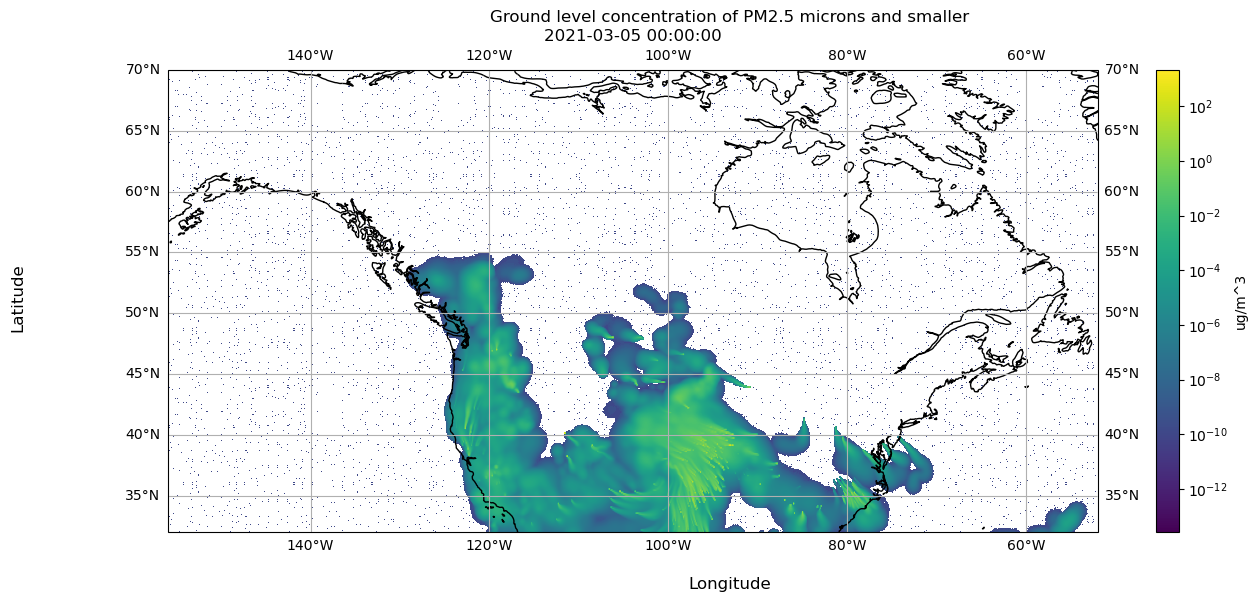
\includegraphics{data_source_files/figure-latex/data_notebooks-data_source-netcdf_demo-cell-13-output-1.png}

\begin{Shaded}
\begin{Highlighting}[]
\NormalTok{ds.close()}
\end{Highlighting}
\end{Shaded}

Now that we understand how to load the data and metadata from the file
and process it for visualization, let's establish the data and metadata
available to us across \emph{all} NetCDF files.

\section{Information Across all NetCDF Files}\label{sec-collection-info}

Knowing what is within one NetCDF file as well as the date range for
which we can download them, let's establish the metadata associated with
the NetCDF files as a \emph{collection}.

\subsection{Disk Size}\label{disk-size}

For the time ranges we cover, Table~\ref{tbl-sizes} shows how large the
set of files per forecast ID are.

\begin{longtable}[]{@{}
  >{\raggedright\arraybackslash}p{(\columnwidth - 6\tabcolsep) * \real{0.2222}}
  >{\raggedright\arraybackslash}p{(\columnwidth - 6\tabcolsep) * \real{0.5139}}
  >{\raggedright\arraybackslash}p{(\columnwidth - 6\tabcolsep) * \real{0.0972}}
  >{\raggedright\arraybackslash}p{(\columnwidth - 6\tabcolsep) * \real{0.1667}}@{}}
\caption{File Sizes and Counts for Each Forecast ID within the Specified
Date Range}\label{tbl-sizes}\tabularnewline
\toprule\noalign{}
\begin{minipage}[b]{\linewidth}\raggedright
Forecast ID
\end{minipage} & \begin{minipage}[b]{\linewidth}\raggedright
Date Range
\end{minipage} & \begin{minipage}[b]{\linewidth}\raggedright
Size
\end{minipage} & \begin{minipage}[b]{\linewidth}\raggedright
File Count
\end{minipage} \\
\midrule\noalign{}
\endfirsthead
\toprule\noalign{}
\begin{minipage}[b]{\linewidth}\raggedright
Forecast ID
\end{minipage} & \begin{minipage}[b]{\linewidth}\raggedright
Date Range
\end{minipage} & \begin{minipage}[b]{\linewidth}\raggedright
Size
\end{minipage} & \begin{minipage}[b]{\linewidth}\raggedright
File Count
\end{minipage} \\
\midrule\noalign{}
\endhead
\bottomrule\noalign{}
\endlastfoot
BSC00CA12-01 & March 4, 2021 - June 27, 2024 & 84G & 1077 \\
BSC06CA12-01 & March 4, 2021 - June 27, 2024 & 78G & 1022 \\
BSC12CA12-01 & March 3, 2021 - June 27, 2024 & 79G & 1022 \\
BSC18CA12-01 & March 4, 2021 - June 27, 2024 & 79G & 1023 \\
\textbf{Total} & & \textbf{320G} & \textbf{4144} \\
\end{longtable}

\subsection{Temporal Data
Availability}\label{temporal-data-availability}

Here we show for what temporal range there is PM25 data available from
the NetCDF files as a \emph{collection}.

\subsubsection{Available Time Ranges}\label{available-time-ranges}

We have downloaded all NetCDF files available within the time ranges
specified by Table~\ref{tbl-time}.

We want to describe exactly what time ranges are covered by each
forecast. We will load the NetCDF file for the date March 3, 2024 for
each forecast ID.

\phantomsection\label{annotated-cell-66}%
\begin{Shaded}
\begin{Highlighting}[]
\NormalTok{file18 }\OperatorTok{=} \SpecialStringTok{f\textquotesingle{}dispersion\_files/18/dispersion\_20210304.nc\textquotesingle{}} \hspace*{\fill}\NormalTok{\circled{1}}
\NormalTok{file00 }\OperatorTok{=} \SpecialStringTok{f\textquotesingle{}dispersion\_files/00/dispersion\_20210304.nc\textquotesingle{}}
\NormalTok{file06 }\OperatorTok{=} \SpecialStringTok{f\textquotesingle{}dispersion\_files/06/dispersion\_20210304.nc\textquotesingle{}}
\NormalTok{file12 }\OperatorTok{=} \SpecialStringTok{f\textquotesingle{}dispersion\_files/12/dispersion\_20210304.nc\textquotesingle{}}
\end{Highlighting}
\end{Shaded}

\begin{description}
\tightlist
\item[\circled{1}]
set paths to files, if you run this demo locally, adjust these as
necessary
\end{description}

\textbf{TODO}

Now that we know what exactly is within a NetCDF file and across all the
NetCDF files, we will continue to describe our data curation process.
Next we describe how we load all of the data available from UBC onto our
machine.

\bookmarksetup{startatroot}

\chapter{References}\label{references-1}

firesmoke.ca website
https://docs.xarray.dev/en/stable/internals/how-to-add-new-backend.html

\bookmarksetup{startatroot}

\chapter{Data Loading}\label{sec-data-loading}

Knowing what data is available and how to obtain the data, we can
proceed with loading the data onto our staging system.

\section{Downloading Data Locally}\label{downloading-data-locally}

We decided to download all the available files from the
\href{data_source.qmd}{data source} onto our \href{sys_specs.qmd}{data
staging machine} to process from there.

We created 4 directories for each forecast ID that UBC provides at the
following directory on our machine:

\begin{verbatim}
/usr/sci/cedmav/data/firesmoke
├── BSC00CA12-01
├── BSC06CA12-01
├── BSC12CA12-01
├── BSC18CA12-01
\end{verbatim}

The following shows our approaches to doing this and discusses how our
approach evolved. Note the scripts below refer to varying directories,
but through simple copying operations we stored the final downloaded
files to the directories listed above.

\subsection{First Approach}\label{first-approach}

We delineate our first approach by detailing our download script, which
is available in it's entirety in the side bar.

\phantomsection\label{annotated-cell-9}%
\begin{Shaded}
\begin{Highlighting}[]
\ImportTok{import}\NormalTok{ wget}
\ImportTok{import}\NormalTok{ pandas }\ImportTok{as}\NormalTok{ pd}

\NormalTok{ids }\OperatorTok{=}\NormalTok{ [}\StringTok{"BSC18CA12{-}01"}\NormalTok{, }\StringTok{"BSC00CA12{-}01"}\NormalTok{, }\StringTok{"BSC06CA12{-}01"}\NormalTok{, }\StringTok{"BSC12CA12{-}01"}\NormalTok{] }\hspace*{\fill}\NormalTok{\circled{1}}
\NormalTok{start\_dates }\OperatorTok{=}\NormalTok{ [}\StringTok{"20210304"}\NormalTok{, }\StringTok{"20210304"}\NormalTok{, }\StringTok{"20210304"}\NormalTok{, }\StringTok{"20210303"}\NormalTok{]}
\NormalTok{end\_dates }\OperatorTok{=}\NormalTok{ [}\StringTok{"20231016"}\NormalTok{, }\StringTok{"20240210"}\NormalTok{, }\StringTok{"20231016"}\NormalTok{, }\StringTok{"20231015"}\NormalTok{]}
\NormalTok{init\_times }\OperatorTok{=}\NormalTok{ [}\StringTok{"02"}\NormalTok{, }\StringTok{"08"}\NormalTok{, }\StringTok{"14"}\NormalTok{, }\StringTok{"20"}\NormalTok{] }

\ControlFlowTok{for}\NormalTok{ i }\KeywordTok{in} \BuiltInTok{zip}\NormalTok{(start\_dates, end\_dates, ids, init\_times): }\hspace*{\fill}\NormalTok{\circled{2}}
\NormalTok{    start\_date }\OperatorTok{=}\NormalTok{ i[}\DecValTok{0}\NormalTok{]}
\NormalTok{    end\_date }\OperatorTok{=}\NormalTok{ i[}\DecValTok{1}\NormalTok{]}
\NormalTok{    forecast\_id }\OperatorTok{=}\NormalTok{ i[}\DecValTok{2}\NormalTok{]}
\NormalTok{    init\_time }\OperatorTok{=}\NormalTok{ i[}\DecValTok{3}\NormalTok{]}

\NormalTok{    dates }\OperatorTok{=}\NormalTok{ pd.date\_range(start}\OperatorTok{=}\NormalTok{start\_date, end}\OperatorTok{=}\NormalTok{end\_date)}
\NormalTok{    dates }\OperatorTok{=}\NormalTok{ dates.strftime(}\StringTok{"\%Y\%m}\SpecialCharTok{\%d}\StringTok{"}\NormalTok{).tolist() }

    \ControlFlowTok{for}\NormalTok{ date }\KeywordTok{in}\NormalTok{ dates: }\hspace*{\fill}\NormalTok{\circled{3}}
\NormalTok{      url }\OperatorTok{=}\NormalTok{ (}
          \StringTok{"https://firesmoke.ca/forecasts/"}
          \OperatorTok{+}\NormalTok{ forecast\_id}
          \OperatorTok{+} \StringTok{"/"}
          \OperatorTok{+}\NormalTok{ date}
          \OperatorTok{+}\NormalTok{ init\_time}
          \OperatorTok{+} \StringTok{"/dispersion.nc"}
\NormalTok{      ) }
\NormalTok{      directory }\OperatorTok{=} \StringTok{"/Users/arleth/Mount/firesmoke/"} \OperatorTok{+}\NormalTok{ forecast\_id }\OperatorTok{+} \StringTok{"/dispersion\_"} \OperatorTok{+}\NormalTok{ date }\OperatorTok{+} \StringTok{".nc"} \hspace*{\fill}\NormalTok{\circled{4}}
\NormalTok{      wget.download(url, out}\OperatorTok{=}\NormalTok{directory) }
\end{Highlighting}
\end{Shaded}

\begin{description}
\tightlist
\item[\circled{1}]
First, create 4 lists containing forecast IDs, the start and end dates
we wish to index on, and the smoke forecast initiation times. We will
loop through the 4 sets of parameters.
\item[\circled{2}]
In a for loop, we use \texttt{pandas} to create a list of every date
from the start date and end date of the current iteration. We will loop
through these dates next.
\item[\circled{3}]
For each \texttt{date} in the list, we create the \texttt{url} to
download the file.
\item[\circled{4}]
Finally, we use \texttt{wget} to download the contents at \texttt{url}to
\texttt{directory}. We append \texttt{date} to the file name so each
file downloaded is identifiable by date.
\end{description}

We assumed that for all URLs, there was an available NetCDF file for
download

However, we realized that we downloaded either a NetCDF file \emph{or an
HTML webpage}. Using \texttt{wget} forcibly saved the contents at the
URL into a NetCDF file.

This issue was not identified until \emph{after} we visualized each hour
of the data, and we noticed gaps and errors in our scripts to create
visualizations. See Chapter~\ref{sec-data-validation} for further
details on identifying these issues. For now, we show our modified
approach to downloading the NetCDF files.

\subsection{Second Approach}\label{second-approach}

Our second approach is similar to the first, except we use
\href{https://requests.readthedocs.io/en/latest/}{\texttt{requests}}, an
HTTP client library that allows us to see the headers returned from the
URL we query. The script is available in the side bar.

\phantomsection\label{annotated-cell-10}%
\begin{Shaded}
\begin{Highlighting}[]
\ImportTok{import}\NormalTok{ requests}
\ImportTok{import}\NormalTok{ pandas }\ImportTok{as}\NormalTok{ pd}
\ImportTok{from}\NormalTok{ datetime }\ImportTok{import}\NormalTok{ datetime}

\NormalTok{ids }\OperatorTok{=}\NormalTok{ [}\StringTok{"BSC18CA12{-}01"}\NormalTok{, }\StringTok{"BSC00CA12{-}01"}\NormalTok{, }\StringTok{"BSC06CA12{-}01"}\NormalTok{, }\StringTok{"BSC12CA12{-}01"}\NormalTok{] }\hspace*{\fill}\NormalTok{\circled{1}}
\NormalTok{start\_dates }\OperatorTok{=}\NormalTok{ [}\StringTok{"20210304"}\NormalTok{, }\StringTok{"20210304"}\NormalTok{, }\StringTok{"20210304"}\NormalTok{, }\StringTok{"20210303"}\NormalTok{]}
\NormalTok{today }\OperatorTok{=}\NormalTok{ datetime.now().strftime(}\StringTok{"\%Y\%m}\SpecialCharTok{\%d}\StringTok{"}\NormalTok{)}
\NormalTok{init\_times }\OperatorTok{=}\NormalTok{ [}\StringTok{"02"}\NormalTok{, }\StringTok{"08"}\NormalTok{, }\StringTok{"14"}\NormalTok{, }\StringTok{"20"}\NormalTok{] }

\ControlFlowTok{for}\NormalTok{ i }\KeywordTok{in} \BuiltInTok{zip}\NormalTok{(start\_dates, ids, init\_times): }\hspace*{\fill}\NormalTok{\circled{2}}
\NormalTok{    start\_date }\OperatorTok{=}\NormalTok{ i[}\DecValTok{0}\NormalTok{]}
\NormalTok{    forecast\_id }\OperatorTok{=}\NormalTok{ i[}\DecValTok{1}\NormalTok{]}
\NormalTok{    init\_time }\OperatorTok{=}\NormalTok{ i[}\DecValTok{2}\NormalTok{]}

\NormalTok{    dates }\OperatorTok{=}\NormalTok{ pd.date\_range(start}\OperatorTok{=}\NormalTok{start\_date, end}\OperatorTok{=}\NormalTok{today)}
\NormalTok{    dates }\OperatorTok{=}\NormalTok{ dates.strftime(}\StringTok{"\%Y\%m}\SpecialCharTok{\%d}\StringTok{"}\NormalTok{).tolist() }

    \ControlFlowTok{for}\NormalTok{ date }\KeywordTok{in}\NormalTok{ dates: }\hspace*{\fill}\NormalTok{\circled{3}}
\NormalTok{        url }\OperatorTok{=}\NormalTok{ (}
            \StringTok{"https://firesmoke.ca/forecasts/"}
            \OperatorTok{+}\NormalTok{ forecast\_id}
            \OperatorTok{+} \StringTok{"/"}
            \OperatorTok{+}\NormalTok{ date}
            \OperatorTok{+}\NormalTok{ init\_time}
            \OperatorTok{+} \StringTok{"/dispersion.nc"}
\NormalTok{        ) }
\NormalTok{        directory }\OperatorTok{=}\NormalTok{ ( }\hspace*{\fill}\NormalTok{\circled{4}}
            \StringTok{"/usr/sci/scratch\_nvme/arleth/basura\_total/"}
            \OperatorTok{+}\NormalTok{ forecast\_id}
            \OperatorTok{+} \StringTok{"/dispersion\_"}
            \OperatorTok{+}\NormalTok{ date}
            \OperatorTok{+} \StringTok{".nc"}
\NormalTok{        ) }

\NormalTok{        response }\OperatorTok{=}\NormalTok{ requests.get(url, stream}\OperatorTok{=}\VariableTok{True}\NormalTok{) }\hspace*{\fill}\NormalTok{\circled{5}}
\NormalTok{        header }\OperatorTok{=}\NormalTok{ response.headers}
        \ControlFlowTok{if}\NormalTok{ (}
            \StringTok{"Content{-}Type"} \KeywordTok{in}\NormalTok{ header}
            \KeywordTok{and}\NormalTok{ header[}\StringTok{"Content{-}Type"}\NormalTok{] }\OperatorTok{==} \StringTok{"application/octet{-}stream"}
\NormalTok{        ): }
            \ControlFlowTok{with} \BuiltInTok{open}\NormalTok{(directory, mode}\OperatorTok{=}\StringTok{"wb"}\NormalTok{) }\ImportTok{as} \BuiltInTok{file}\NormalTok{: }\hspace*{\fill}\NormalTok{\circled{6}}
                \BuiltInTok{file}\NormalTok{.write(response.content)}
                \BuiltInTok{print}\NormalTok{(}\SpecialStringTok{f"Downloaded file }\SpecialCharTok{\{}\NormalTok{directory}\SpecialCharTok{\}}\SpecialStringTok{"}\NormalTok{)}
        \ControlFlowTok{else}\NormalTok{:}
            \BuiltInTok{print}\NormalTok{(header[}\StringTok{"Content{-}Type"}\NormalTok{]) }
\end{Highlighting}
\end{Shaded}

\begin{description}
\tightlist
\item[\circled{1}]
First, create 3 lists containing forecast IDs, the start dates we wish
to index on, and the smoke forecast initiation times . Notice we define
a variable \texttt{today}, this allows us to run this script and query
all URLs up to today's date. Note we ran up to June 27, 2024 for now. We
will loop through these sets of parameters.
\item[\circled{2}]
In a for loop, we use \texttt{pandas} to create a list of every date
from the start date and end date of the current iteration. We will loop
through these dates next.
\item[\circled{3}]
For each \texttt{date} in the list, we create the \texttt{url} to
download the file.
\item[\circled{4}]
Define \texttt{directory}, the directory and file name to save the file
to.
\item[\circled{5}]
We use \texttt{requests} to get the HTTP header at \texttt{url}. We
inspect the \texttt{Content-Type} and if it is
\texttt{application/octet-stream}, we download the file. We confirmed
that a URL with a NetCDF file had this content type header.
\item[\circled{6}]
We write the content to \texttt{directory}, else we print the content
header out to check what it is.
\end{description}

This approach yielded the results we expected, we downloaded only NetCDF
files. We had failed downloads which appeared during conversion as
described in Chapter~\ref{sec-data-conversion}. We assumed those files
were unavailable from UBC which we later confirmed as described in
Chapter~\ref{sec-data-validation}.

\bookmarksetup{startatroot}

\chapter{Data Conversion}\label{sec-data-conversion}

So far, we have established what the data from UBC is and how to
download it to our machine. Now we describe how to compile the data on
our machine into an IDX file using the
\href{https://github.com/sci-visus/OpenVisus/tree/master}{OpenViSUS
libary} and its access to the
\href{https://github.com/sci-visus/PIDX?tab=readme-ov-file}{PIDX
library}.

\section{On Data Validation}\label{on-data-validation}

We decided to perform data validation \emph{after} conversion to the IDX
file format. However, we realized that performing data validation
\emph{both before and after} conversion would be best. This is explored
further in Chapter~\ref{sec-data-validation}.

For now, the reader should understand that data validation of the NetCDF
files is different from data validation of the IDX file. In this
chapter, we use the assumption that the NetCDF files \emph{we can open}
have complete and uncorrupted data for conversion to IDX.

\section{Overview}\label{overview-1}

For all our conversion script versions, the same general process is
followed:

\begin{enumerate}
\def\labelenumi{\arabic{enumi}.}
\tightlist
\item
  Check which NetCDF files were successfully downloaded from the data
  source by attempting to open each downloaded file with
  \texttt{xarray}.
\item
  Obtain a subset of data from the files to create a dataset of
  chronological, hour by hour, data.
\item
  Save this time series data to an \texttt{IDX} file using the
  \href{https://github.com/sci-visus/OpenVisus/tree/master}{OpenVisus}
  framework.
\end{enumerate}

We will describe the latest version of our conversion, \textbf{version
4}. Throughout, we will explain how previous attempts were deficient.

To see previous attemps in their entirety, refer to the side bar. Please
note that the previous scripts were working scripts, therefore they may
be incomplete.

\section{Setting System Directories}\label{setting-system-directories}

First we set the directory paths we want to use during the conversion
process, which is to our 4 directories of NetCDF files for each forecast
ID.

\phantomsection\label{annotated-cell-12}%
\begin{Shaded}
\begin{Highlighting}[]
\NormalTok{firesmoke\_dir }\OperatorTok{=} \StringTok{"/usr/sci/cedmav/data/firesmoke"} \hspace*{\fill}\NormalTok{\circled{1}}
\NormalTok{idx\_dir }\OperatorTok{=} \StringTok{"/usr/sci/scratch\_nvme/arleth/idx/firesmoke"} 

\NormalTok{ids }\OperatorTok{=}\NormalTok{ [}\StringTok{"BSC18CA12{-}01"}\NormalTok{, }\StringTok{"BSC00CA12{-}01"}\NormalTok{, }\StringTok{"BSC06CA12{-}01"}\NormalTok{, }\StringTok{"BSC12CA12{-}01"}\NormalTok{] }\hspace*{\fill}\NormalTok{\circled{2}}
\NormalTok{start\_dates }\OperatorTok{=}\NormalTok{ [}\StringTok{"20210304"}\NormalTok{, }\StringTok{"20210304"}\NormalTok{, }\StringTok{"20210304"}\NormalTok{, }\StringTok{"20210303"}\NormalTok{] }
\NormalTok{end\_dates }\OperatorTok{=}\NormalTok{ [}\StringTok{"20240627"}\NormalTok{, }\StringTok{"20240627"}\NormalTok{, }\StringTok{"20240627"}\NormalTok{, }\StringTok{"20240627"}\NormalTok{] }
\end{Highlighting}
\end{Shaded}

\begin{description}
\tightlist
\item[\circled{1}]
Establish the directory where all forecast ID NetCDFs are stored and
where to save our IDX file on the `atlantis' machine.
\item[\circled{2}]
Define the forecast IDs and dates we will loop over.
\end{description}

\subsection{Rationale and Future
Improvements}\label{rationale-and-future-improvements}

\subsubsection{Data Usage}\label{data-usage}

In versions 1 and 2 of our conversion attempt, we did not use all four
sets of forecast ID files. We only used BSC12CA12-01 files to compile a
single dataset. We learned that by not using all four sets of data, the
dataset we created was less accurate. See
Chapter~\ref{sec-data-validation} for further details.

Therefore we decided to use all four datasets, see
Section~\ref{sec-sequencing} for details. We elect to use dates up to
June 27, 2024 as this was the last time we ran our scripts. We have yet
to address the issue of how to keep the IDX file constantly up to date
with data available up to the present day.

\section{Checking the NetCDF Files}\label{checking-the-netcdf-files}

Recall we downloaded all NetCDF files available from UBC onto our
machine in their respective directories as follows:

\begin{verbatim}
/usr/sci/cedmav/data/firesmoke
├── BSC00CA12-01
├── BSC06CA12-01
├── BSC12CA12-01
├── BSC18CA12-01
\end{verbatim}

Here, we identify which NetCDF files for each forecast ID successfully
open with \texttt{xarray} and store them in a dictionary.

We also confirm the following conditions we established in
Chapter~\ref{sec-data-source} by using dictionaries to track the max
values and unique values of these attributes across all files:

\begin{enumerate}
\def\labelenumi{\arabic{enumi}.}
\tightlist
\item
  All files across all four forecast IDs have the same \texttt{NROWS},
  \texttt{XORIG}, \texttt{YORIG}, \texttt{XCELL}, \texttt{YCELL} values.
\item
  Some files have either \texttt{NCOLS\ =\ 1041} or
  \texttt{NCOLS\ =\ 1081}, but always \texttt{NROWS\ =\ 381}.
\end{enumerate}

\phantomsection\label{annotated-cell-14}%
\begin{Shaded}
\begin{Highlighting}[]
\ImportTok{import}\NormalTok{ os}
\ImportTok{import}\NormalTok{ xarray }\ImportTok{as}\NormalTok{ xr}
\ImportTok{import}\NormalTok{ numpy }\ImportTok{as}\NormalTok{ np}
\ImportTok{import}\NormalTok{ tqdm}

\NormalTok{successful\_files }\OperatorTok{=}\NormalTok{ \{id\_: [] }\ControlFlowTok{for}\NormalTok{ id\_ }\KeywordTok{in}\NormalTok{ ids\} }\hspace*{\fill}\NormalTok{\circled{1}}

\NormalTok{max\_ncols }\OperatorTok{=}\NormalTok{ \{id\_: }\DecValTok{0} \ControlFlowTok{for}\NormalTok{ id\_ }\KeywordTok{in}\NormalTok{ ids\} }\hspace*{\fill}\NormalTok{\circled{2}}
\NormalTok{max\_nrows }\OperatorTok{=}\NormalTok{ \{id\_: }\DecValTok{0} \ControlFlowTok{for}\NormalTok{ id\_ }\KeywordTok{in}\NormalTok{ ids\} }
\NormalTok{ncols }\OperatorTok{=}\NormalTok{ \{id\_: }\BuiltInTok{set}\NormalTok{() }\ControlFlowTok{for}\NormalTok{ id\_ }\KeywordTok{in}\NormalTok{ ids\} }\hspace*{\fill}\NormalTok{\circled{3}}
\NormalTok{nrows }\OperatorTok{=}\NormalTok{ \{id\_: }\BuiltInTok{set}\NormalTok{() }\ControlFlowTok{for}\NormalTok{ id\_ }\KeywordTok{in}\NormalTok{ ids\} }

\NormalTok{max\_grid\_x }\OperatorTok{=}\NormalTok{ \{id\_: \{}\StringTok{"xorig"}\NormalTok{: }\FloatTok{0.0}\NormalTok{, }\StringTok{"xcell"}\NormalTok{: }\FloatTok{0.0}\NormalTok{\} }\ControlFlowTok{for}\NormalTok{ id\_ }\KeywordTok{in}\NormalTok{ ids\} }\hspace*{\fill}\NormalTok{\circled{4}}
\NormalTok{max\_grid\_y }\OperatorTok{=}\NormalTok{ \{id\_: \{}\StringTok{"yorig"}\NormalTok{: }\FloatTok{0.0}\NormalTok{, }\StringTok{"ycell"}\NormalTok{: }\FloatTok{0.0}\NormalTok{\} }\ControlFlowTok{for}\NormalTok{ id\_ }\KeywordTok{in}\NormalTok{ ids\} }
\NormalTok{xorigs }\OperatorTok{=}\NormalTok{ \{id\_: }\BuiltInTok{set}\NormalTok{() }\ControlFlowTok{for}\NormalTok{ id\_ }\KeywordTok{in}\NormalTok{ ids\} }\hspace*{\fill}\NormalTok{\circled{5}}
\NormalTok{xcells }\OperatorTok{=}\NormalTok{ \{id\_: }\BuiltInTok{set}\NormalTok{() }\ControlFlowTok{for}\NormalTok{ id\_ }\KeywordTok{in}\NormalTok{ ids\}}
\NormalTok{yorigs }\OperatorTok{=}\NormalTok{ \{id\_: }\BuiltInTok{set}\NormalTok{() }\ControlFlowTok{for}\NormalTok{ id\_ }\KeywordTok{in}\NormalTok{ ids\}}
\NormalTok{ycells }\OperatorTok{=}\NormalTok{ \{id\_: }\BuiltInTok{set}\NormalTok{() }\ControlFlowTok{for}\NormalTok{ id\_ }\KeywordTok{in}\NormalTok{ ids\} }

\ControlFlowTok{for}\NormalTok{ id\_ }\KeywordTok{in}\NormalTok{ ids: }\hspace*{\fill}\NormalTok{\circled{6}}
\NormalTok{    file\_names }\OperatorTok{=}\NormalTok{ os.listdir(}\SpecialStringTok{f"}\SpecialCharTok{\{}\NormalTok{firesmoke\_dir}\SpecialCharTok{\}}\SpecialStringTok{/}\SpecialCharTok{\{}\NormalTok{id\_}\SpecialCharTok{\}}\SpecialStringTok{/"}\NormalTok{) }\hspace*{\fill}\NormalTok{\circled{7}}

    \ControlFlowTok{for} \BuiltInTok{file} \KeywordTok{in}\NormalTok{ tqdm(file\_names): }\hspace*{\fill}\NormalTok{\circled{8}}
\NormalTok{        path }\OperatorTok{=} \SpecialStringTok{f"}\SpecialCharTok{\{}\NormalTok{firesmoke\_dir}\SpecialCharTok{\}}\SpecialStringTok{/}\SpecialCharTok{\{}\NormalTok{id\_}\SpecialCharTok{\}}\SpecialStringTok{/}\SpecialCharTok{\{}\BuiltInTok{file}\SpecialCharTok{\}}\SpecialStringTok{"} \hspace*{\fill}\NormalTok{\circled{9}}

        \ControlFlowTok{try}\NormalTok{: }\hspace*{\fill}\NormalTok{\circled{10}}
\NormalTok{            ds }\OperatorTok{=}\NormalTok{ xr.open\_dataset(path) }

\NormalTok{            successful\_files[id\_].append(}\BuiltInTok{file}\NormalTok{) }\hspace*{\fill}\NormalTok{\circled{11}}

\NormalTok{            max\_ncols[id\_] }\OperatorTok{=} \BuiltInTok{max}\NormalTok{(max\_ncols[id\_], ds.NCOLS) }\hspace*{\fill}\NormalTok{\circled{12}}
\NormalTok{            max\_nrows[id\_] }\OperatorTok{=} \BuiltInTok{max}\NormalTok{(max\_nrows[id\_], ds.NROWS)}
\NormalTok{            max\_grid\_x[id\_][}\StringTok{"xorig"}\NormalTok{] }\OperatorTok{=} \BuiltInTok{max}\NormalTok{(max\_grid\_x[id\_][}\StringTok{"xorig"}\NormalTok{], ds.XORIG, key}\OperatorTok{=}\BuiltInTok{abs}\NormalTok{)}
\NormalTok{            max\_grid\_y[id\_][}\StringTok{"yorig"}\NormalTok{] }\OperatorTok{=} \BuiltInTok{max}\NormalTok{(max\_grid\_y[id\_][}\StringTok{"yorig"}\NormalTok{], ds.YORIG, key}\OperatorTok{=}\BuiltInTok{abs}\NormalTok{)}
\NormalTok{            max\_grid\_x[id\_][}\StringTok{"xcell"}\NormalTok{] }\OperatorTok{=} \BuiltInTok{max}\NormalTok{(max\_grid\_x[id\_][}\StringTok{"xcell"}\NormalTok{], ds.XCELL, key}\OperatorTok{=}\BuiltInTok{abs}\NormalTok{)}
\NormalTok{            max\_grid\_y[id\_][}\StringTok{"ycell"}\NormalTok{] }\OperatorTok{=} \BuiltInTok{max}\NormalTok{(}
\NormalTok{                max\_grid\_y[id\_][}\StringTok{"ycell"}\NormalTok{], ds.YCELL, key}\OperatorTok{=}\BuiltInTok{abs}
\NormalTok{            ) }

\NormalTok{            ncols[id\_].add(ds.NCOLS) }\hspace*{\fill}\NormalTok{\circled{13}}
\NormalTok{            nrows[id\_].add(ds.NROWS)}
\NormalTok{            xorigs[id\_].add(ds.XORIG)}
\NormalTok{            yorigs[id\_].add(ds.YORIG)}
\NormalTok{            xcells[id\_].add(ds.XCELL)}
\NormalTok{            ycells[id\_].add(ds.YCELL) }

        \ControlFlowTok{except}\NormalTok{: }\hspace*{\fill}\NormalTok{\circled{14}}
            \ControlFlowTok{continue}

\ControlFlowTok{for}\NormalTok{ id\_ }\KeywordTok{in}\NormalTok{ successful\_files: }\hspace*{\fill}\NormalTok{\circled{15}}
\NormalTok{    successful\_files[id\_] }\OperatorTok{=}\NormalTok{ np.sort(successful\_files[id\_]).tolist() }
\end{Highlighting}
\end{Shaded}

\begin{description}
\tightlist
\item[\circled{1}]
Initialize a dictionary to hold an empty list for each forecast ID. We
update it with the file names that successfully open under the forecast
ID directory.
\item[\circled{2}]
Initialize dictionaries to hold an integer for each forecast ID. We
update it to hold the maximum \texttt{NCOLS}/\texttt{NROWS} value
available within forecast ID's set of NetCDF files.
\item[\circled{3}]
Initialize dictionaries to hold a set for each forecast ID. We update
the set to hold all the unique \texttt{NCOLS}/\texttt{NROWS} values
available within the forecast ID's set of NetCDF files.
\item[\circled{4}]
Initialize dictionaries to hold a dictionary of
\texttt{xorig}/\texttt{yorig} and \texttt{xcell}/\texttt{ycell} values
for each forecast ID. We update it to hold the maximum
\texttt{xorig}/\texttt{yorig} and \texttt{xcell}/\texttt{ycell} pairs
available within the forecast ID's set of NetCDF files.
\item[\circled{5}]
Initialize dictionaries to track unique \texttt{xorig}/\texttt{yorig}
and \texttt{xcell}/\texttt{ycell} values.
\item[\circled{6}]
For each forecast ID, we populate the dictionaries above.
\item[\circled{7}]
Obtain a list of file names under the directory for \texttt{id\_}. We
loop through each file next.
\item[\circled{8}]
Begin loop over each file. Note \texttt{tqdm} is just an accessory for
generating a visible status bar in our Jupyter Notebook.
\item[\circled{9}]
Obtain absolute path name to current file.
\item[\circled{10}]
Here we use a \texttt{try} statement since opening the file with
\texttt{xarray} may lead to an error. \texttt{except} allows us to catch
the exception accordingly and continue trying to open each file.
\item[\circled{11}]
At this line, the file opened without issue in \texttt{xarray}, so
append this file name to the \texttt{id\_} list in the
\texttt{successful\_files} dictionary.
\item[\circled{12}]
Use \texttt{max} to save the largest values in our dictionaries
accordingly.
\item[\circled{13}]
Update the dictionaries of sets with the file's attributes, to ensure we
catch all unique values.
\item[\circled{14}]
If the file did not open during the \texttt{try} continue to the next
file.
\item[\circled{15}]
Sort the lists of successfully opened files by name, so they are in
chronological order.
\end{description}

The following shows the information gathered:

\section{BSC18CA12-01}

\begin{verbatim}
dataset: BSC18CA12-01
Number of successful files: 1010
Max cell sizes: max_ncols = 1081 and max_nrows = 381
Max xorig & xcell: {'xorig': -160.0, 'xcell': 0.10000000149011612}
Max yorig & ycell: {'yorig': 32.0, 'ycell': 0.10000000149011612}
ncols: {1081, 1041}
nrows: {381}
xorigs: {-160.0, -156.0}
yorigs: {32.0}
xcells: {0.10000000149011612}
ycells: {0.10000000149011612}
\end{verbatim}

\section{BSC00CA12-01}

\begin{verbatim}
dataset: BSC00CA12-01
Number of successful files: 1067
Max cell sizes: max_ncols = 1081 and max_nrows = 381
Max xorig & xcell: {'xorig': -160.0, 'xcell': 0.10000000149011612}
Max yorig & ycell: {'yorig': 32.0, 'ycell': 0.10000000149011612}
ncols: {1081, 1041}
nrows: {381}
xorigs: {-160.0, -156.0}
yorigs: {32.0}
xcells: {0.10000000149011612}
ycells: {0.10000000149011612}
\end{verbatim}

\section{BSC06CA12-01}

\begin{verbatim}
dataset: BSC06CA12-01
Number of successful files: 997
Max cell sizes: max_ncols = 1081 and max_nrows = 381
Max xorig & xcell: {'xorig': -160.0, 'xcell': 0.10000000149011612}
Max yorig & ycell: {'yorig': 32.0, 'ycell': 0.10000000149011612}
ncols: {1081, 1041}
nrows: {381}
xorigs: {-160.0, -156.0}
yorigs: {32.0}
xcells: {0.10000000149011612}
ycells: {0.10000000149011612}
\end{verbatim}

\section{BSC12CA12-01}

\begin{verbatim}
dataset: BSC12CA12-01
Number of successful files: 1003
Max cell sizes: max_ncols = 1081 and max_nrows = 381
Max xorig & xcell: {'xorig': -160.0, 'xcell': 0.10000000149011612}
Max yorig & ycell: {'yorig': 32.0, 'ycell': 0.10000000149011612}
ncols: {1081, 1041}
nrows: {381}
xorigs: {-160.0, -156.0}
yorigs: {32.0}
xcells: {0.10000000149011612}
ycells: {0.10000000149011612}
\end{verbatim}

\subsection{Rationale and Future
Improvements}\label{rationale-and-future-improvements-1}

\subsubsection{Unloadable Files}\label{unloadable-files}

On our first attempt to convert the data we discovered that various
files failed to open. Therefore, we used a dictionary to keep track of
which files successfully open.

\subsubsection{Varying Grid Size}\label{varying-grid-size}

In this step we collect attribute information about the two different
grids used in the dataset. We proceed to use these attributes to
resample the grids accordingly, see Section~\ref{sec-resampling}.

\subsubsection{Optimization and Scaling}\label{optimization-and-scaling}

One improvement to this step is to stop tracking maxes and unique values
seperately. Instead, we could just track unique values then get maxes
from there. Furthermore, modularizing this process such that it handles
the possibility of new grids being used in the dataset would make the
conversion script more scalable.

\section{Preparing Resampling Grids}\label{sec-resampling}

Now that we have the sets of openable files, we begin to handle the need
to resample data. To resample arrays of shape 381×1041 to 381×1081, we
use the SciPy \texttt{griddata} function from the \texttt{interpolate}
package. This function gives interpolated values on set of points
\texttt{xi} from a set of \texttt{points} with corresponding
\texttt{values}. We refer the reader to SciPy's
\href{https://docs.scipy.org/doc/scipy/reference/generated/scipy.interpolate.griddata.html}{documentation}
for details.

In this step, we obtain the grids we wish to use as our \texttt{points}
and \texttt{xi}. See Section~\ref{sec-resample-example} for how we use
these grids with the \texttt{griddata} function.

\subsection{Generate Grids of Latitude and Longitude
Points}\label{generate-grids-of-latitude-and-longitude-points}

Recall we can generate a set of latitude and longitude coordinates by
using the attributes given in each NetCDF file, see
Section~\ref{sec-netcdf-demo} for an example. Here we generate two sets
of latitude and longitude coordinates for each grid size.

\phantomsection\label{annotated-cell-15}%
\begin{Shaded}
\begin{Highlighting}[]
\NormalTok{max\_xorig }\OperatorTok{=}\NormalTok{ max\_grid\_x[ids[}\DecValTok{0}\NormalTok{]][}\StringTok{\textquotesingle{}xorig\textquotesingle{}}\NormalTok{] }\hspace*{\fill}\NormalTok{\circled{1}}
\NormalTok{max\_xcell }\OperatorTok{=}\NormalTok{ max\_grid\_x[ids[}\DecValTok{0}\NormalTok{]][}\StringTok{\textquotesingle{}xcell\textquotesingle{}}\NormalTok{]}
\NormalTok{max\_yorig }\OperatorTok{=}\NormalTok{ max\_grid\_y[ids[}\DecValTok{0}\NormalTok{]][}\StringTok{\textquotesingle{}yorig\textquotesingle{}}\NormalTok{]}
\NormalTok{max\_ycell }\OperatorTok{=}\NormalTok{ max\_grid\_y[ids[}\DecValTok{0}\NormalTok{]][}\StringTok{\textquotesingle{}ycell\textquotesingle{}}\NormalTok{] }

\NormalTok{big\_lon }\OperatorTok{=}\NormalTok{ np.linspace(max\_xorig, max\_xorig }\OperatorTok{+}\NormalTok{ max\_xcell }\OperatorTok{*}\NormalTok{ (max\_ncols[ids[}\DecValTok{0}\NormalTok{]] }\OperatorTok{{-}} \DecValTok{1}\NormalTok{), max\_ncols[ids[}\DecValTok{0}\NormalTok{]]) }\hspace*{\fill}\NormalTok{\circled{2}}
\NormalTok{big\_lat }\OperatorTok{=}\NormalTok{ np.linspace(max\_yorig, max\_yorig }\OperatorTok{+}\NormalTok{ max\_ycell }\OperatorTok{*}\NormalTok{ (max\_nrows[ids[}\DecValTok{0}\NormalTok{]] }\OperatorTok{{-}} \DecValTok{1}\NormalTok{), max\_nrows[ids[}\DecValTok{0}\NormalTok{]]) }

\NormalTok{big\_lon\_pts, big\_lat\_pts }\OperatorTok{=}\NormalTok{ np.meshgrid(big\_lon, big\_lat) }\hspace*{\fill}\NormalTok{\circled{3}}
\NormalTok{big\_tups }\OperatorTok{=}\NormalTok{ np.array([tup }\ControlFlowTok{for}\NormalTok{ tup }\KeywordTok{in} \BuiltInTok{zip}\NormalTok{(big\_lon\_pts.flatten(), big\_lat\_pts.flatten())]) }

\NormalTok{sml\_ds }\OperatorTok{=}\NormalTok{ xr.open\_dataset(firesmoke\_dir }\OperatorTok{+} \StringTok{"/BSC00CA12{-}01/dispersion\_20210304.nc"}\NormalTok{) }\hspace*{\fill}\NormalTok{\circled{4}}
\NormalTok{sml\_lon }\OperatorTok{=}\NormalTok{ np.linspace(sml\_ds.XORIG, sml\_ds.XORIG }\OperatorTok{+}\NormalTok{ sml\_ds.XCELL }\OperatorTok{*}\NormalTok{ (sml\_ds.NCOLS }\OperatorTok{{-}} \DecValTok{1}\NormalTok{), sml\_ds.NCOLS)}
\NormalTok{sml\_lat }\OperatorTok{=}\NormalTok{ np.linspace(sml\_ds.YORIG, sml\_ds.YORIG }\OperatorTok{+}\NormalTok{ sml\_ds.YCELL }\OperatorTok{*}\NormalTok{ (sml\_ds.NROWS }\OperatorTok{{-}} \DecValTok{1}\NormalTok{), sml\_ds.NROWS) }

\NormalTok{sml\_lon\_pts, sml\_lat\_pts }\OperatorTok{=}\NormalTok{ np.meshgrid(sml\_lon, sml\_lat) }\hspace*{\fill}\NormalTok{\circled{5}}
\NormalTok{sml\_tups }\OperatorTok{=}\NormalTok{ np.array([tup }\ControlFlowTok{for}\NormalTok{ tup }\KeywordTok{in} \BuiltInTok{zip}\NormalTok{(sml\_lon\_pts.flatten(), sml\_lat\_pts.flatten())]) }
\end{Highlighting}
\end{Shaded}

\begin{description}
\tightlist
\item[\circled{1}]
Get the x/y origin and cell size parameters for the big 381×1081 grid.
\item[\circled{2}]
Generate one two lists, defining a grid of latitudes and longitudes.
\item[\circled{3}]
Using \texttt{big\_lon} and \texttt{big\_lat}, use meshgrid to generate
our 381×1081 set of longitudes and latitudes.
\item[\circled{4}]
Open a file that uses the small 381×1041 grid. Then, use the attributes
in that file to generate two lists defining a grid of latitudes and
longitudes.
\item[\circled{5}]
Using \texttt{sml\_lon} and \texttt{sml\_lat}, use meshgrid to generate
our 381×1041 set of longitudes and latitudes.
\end{description}

See below for an example of using these latitude and longitude grids to
resample data on a 381×1041 grid to a 381×1081 grid.

\subsection{\texorpdfstring{Example with
\texttt{griddata}}{Example with griddata}}\label{sec-resample-example}

Now that we have the two sets of latitude and longitude points, we show
an example of how these are used to resample an array of data from a
381×1041 grid to a 381×1081 grid.

In this example we use the latitude and longitude points generated from
the attributes determine across all NetCDF files.

\begin{Shaded}
\begin{Highlighting}[]
\ImportTok{import}\NormalTok{ numpy }\ImportTok{as}\NormalTok{ np}
\ImportTok{import}\NormalTok{ xarray }\ImportTok{as}\NormalTok{ xr}
\end{Highlighting}
\end{Shaded}

\phantomsection\label{annotated-cell-72}%
\begin{Shaded}
\begin{Highlighting}[]
\NormalTok{max\_xorig }\OperatorTok{=} \OperatorTok{{-}}\FloatTok{160.0} \hspace*{\fill}\NormalTok{\circled{1}}
\NormalTok{max\_xcell }\OperatorTok{=} \FloatTok{0.10000000149011612} \hspace*{\fill}\NormalTok{\circled{2}}
\NormalTok{max\_yorig }\OperatorTok{=} \FloatTok{32.0} \hspace*{\fill}\NormalTok{\circled{3}}
\NormalTok{max\_ycell }\OperatorTok{=} \FloatTok{0.10000000149011612} \hspace*{\fill}\NormalTok{\circled{4}}

\NormalTok{big\_lon }\OperatorTok{=}\NormalTok{ np.linspace(max\_xorig, max\_xorig }\OperatorTok{+}\NormalTok{ max\_xcell }\OperatorTok{*}\NormalTok{ (}\DecValTok{1081} \OperatorTok{{-}} \DecValTok{1}\NormalTok{), }\DecValTok{1081}\NormalTok{) }\hspace*{\fill}\NormalTok{\circled{5}}
\NormalTok{big\_lat }\OperatorTok{=}\NormalTok{ np.linspace(max\_yorig, max\_yorig }\OperatorTok{+}\NormalTok{ max\_ycell }\OperatorTok{*}\NormalTok{ (}\DecValTok{381} \OperatorTok{{-}} \DecValTok{1}\NormalTok{), }\DecValTok{381}\NormalTok{) }\hspace*{\fill}\NormalTok{\circled{6}}

\NormalTok{big\_lon\_pts, big\_lat\_pts }\OperatorTok{=}\NormalTok{ np.meshgrid(big\_lon, big\_lat) }\hspace*{\fill}\NormalTok{\circled{7}}
\NormalTok{big\_tups }\OperatorTok{=}\NormalTok{ np.array([tup }\ControlFlowTok{for}\NormalTok{ tup }\KeywordTok{in} \BuiltInTok{zip}\NormalTok{(big\_lon\_pts.flatten(), big\_lat\_pts.flatten())]) }\hspace*{\fill}\NormalTok{\circled{8}}

\NormalTok{sml\_ds }\OperatorTok{=}\NormalTok{ xr.open\_dataset(}\StringTok{"dispersion\_20210304.nc"}\NormalTok{) }\hspace*{\fill}\NormalTok{\circled{9}}
\NormalTok{sml\_lon }\OperatorTok{=}\NormalTok{ np.linspace(sml\_ds.XORIG, sml\_ds.XORIG }\OperatorTok{+}\NormalTok{ sml\_ds.XCELL }\OperatorTok{*}\NormalTok{ (sml\_ds.NCOLS }\OperatorTok{{-}} \DecValTok{1}\NormalTok{), sml\_ds.NCOLS) }\hspace*{\fill}\NormalTok{\circled{10}}
\NormalTok{sml\_lat }\OperatorTok{=}\NormalTok{ np.linspace(sml\_ds.YORIG, sml\_ds.YORIG }\OperatorTok{+}\NormalTok{ sml\_ds.YCELL }\OperatorTok{*}\NormalTok{ (sml\_ds.NROWS }\OperatorTok{{-}} \DecValTok{1}\NormalTok{), sml\_ds.NROWS) }\hspace*{\fill}\NormalTok{\circled{11}}

\NormalTok{sml\_lon\_pts, sml\_lat\_pts }\OperatorTok{=}\NormalTok{ np.meshgrid(sml\_lon, sml\_lat) }\hspace*{\fill}\NormalTok{\circled{12}}
\NormalTok{sml\_tups }\OperatorTok{=}\NormalTok{ np.array([tup }\ControlFlowTok{for}\NormalTok{ tup }\KeywordTok{in} \BuiltInTok{zip}\NormalTok{(sml\_lon\_pts.flatten(), sml\_lat\_pts.flatten())]) }\hspace*{\fill}\NormalTok{\circled{13}}
\end{Highlighting}
\end{Shaded}

\begin{description}
\tightlist
\item[\circled{1}]
Define the maximum x-origin coordinate.
\item[\circled{2}]
Define the maximum x-cell size.
\item[\circled{3}]
Define the maximum y-origin coordinate.
\item[\circled{4}]
Define the maximum y-cell size.
\item[\circled{5}]
Create an array for the large longitude grid.
\item[\circled{6}]
Create an array for the large latitude grid.
\item[\circled{7}]
Create a meshgrid of points using the large longitude and latitude
arrays.
\item[\circled{8}]
Create a flattened array of tuples representing the large grid points.
\item[\circled{9}]
Open the small dataset using xarray.
\item[\circled{10}]
Create an array for the small longitude grid.
\item[\circled{11}]
Create an array for the small latitude grid.
\item[\circled{12}]
Create a meshgrid of points using the small longitude and latitude
arrays.
\item[\circled{13}]
Create a flattened array of tuples representing the small grid points.
\end{description}

\begin{Shaded}
\begin{Highlighting}[]
\BuiltInTok{print}\NormalTok{(}\SpecialStringTok{f\textquotesingle{}Using the large grid, we have }\SpecialCharTok{\{}\NormalTok{np}\SpecialCharTok{.}\NormalTok{shape(big\_tups)[}\DecValTok{0}\NormalTok{]}\SpecialCharTok{\}}\SpecialStringTok{ lat/lon points to sample on.\textquotesingle{}}\NormalTok{)}
\BuiltInTok{print}\NormalTok{(}\SpecialStringTok{f\textquotesingle{}Using the small grid, we have }\SpecialCharTok{\{}\NormalTok{np}\SpecialCharTok{.}\NormalTok{shape(sml\_tups)[}\DecValTok{0}\NormalTok{]}\SpecialCharTok{\}}\SpecialStringTok{ lat/lon points to sample from.\textquotesingle{}}\NormalTok{)}
\end{Highlighting}
\end{Shaded}

\begin{verbatim}
Using the large grid, we have 411861 lat/lon points to sample on.
Using the small grid, we have 396621 lat/lon points to sample from.
\end{verbatim}

Let's get the data at timestep 0 inside
\texttt{dispersion\_20210304.nc}, which uses a grid of size 381×1041.

\begin{Shaded}
\begin{Highlighting}[]
\NormalTok{timestep }\OperatorTok{=} \DecValTok{0}

\NormalTok{vals }\OperatorTok{=}\NormalTok{ np.squeeze(sml\_ds[}\StringTok{\textquotesingle{}PM25\textquotesingle{}}\NormalTok{].values)}

\BuiltInTok{print}\NormalTok{(}\SpecialStringTok{f\textquotesingle{}The shape of the PM25 array at timestep }\SpecialCharTok{\{}\NormalTok{timestep}\SpecialCharTok{\}}\SpecialStringTok{ is }\SpecialCharTok{\{}\NormalTok{np}\SpecialCharTok{.}\NormalTok{shape(vals[timestep])}\SpecialCharTok{\}}\SpecialStringTok{\textquotesingle{}}\NormalTok{)}
\end{Highlighting}
\end{Shaded}

\begin{verbatim}
The shape of the PM25 array at timestep 0 is (381, 1041)
\end{verbatim}

We use the following parameters with
\href{https://docs.scipy.org/doc/scipy/reference/generated/scipy.interpolate.griddata.html}{\texttt{griddata}}
to resample \texttt{vals}:

\texttt{griddata(points,\ values,\ xi,\ method=\textquotesingle{}cubic\textquotesingle{},\ fill\_value)}

\begin{itemize}
\tightlist
\item
  \texttt{points}: Data point coordinates.
\item
  \texttt{values}: Data values.
\item
  \texttt{xi}: Points at which to interpolate data.
\item
  \texttt{method}: cubic, 2D: Return the value determined from a
  piecewise cubic, continuously differentiable (C1), and approximately
  curvature-minimizing polynomial surface.
\item
  \texttt{fill\_value}: Value used to fill in for requested points
  outside of the convex hull of the input points.
\end{itemize}

\phantomsection\label{annotated-cell-75}%
\begin{Shaded}
\begin{Highlighting}[]
\ImportTok{from}\NormalTok{ scipy.interpolate }\ImportTok{import}\NormalTok{ griddata}

\NormalTok{points }\OperatorTok{=}\NormalTok{ sml\_tups }\hspace*{\fill}\NormalTok{\circled{1}}
\NormalTok{values }\OperatorTok{=}\NormalTok{ vals[timestep].flatten() }\hspace*{\fill}\NormalTok{\circled{2}}
\NormalTok{xi }\OperatorTok{=}\NormalTok{ big\_tups }\hspace*{\fill}\NormalTok{\circled{3}}
\NormalTok{method }\OperatorTok{=} \StringTok{\textquotesingle{}cubic\textquotesingle{}} \hspace*{\fill}\NormalTok{\circled{4}}
\NormalTok{fill\_value }\OperatorTok{=} \DecValTok{0} \hspace*{\fill}\NormalTok{\circled{5}}

\NormalTok{arr }\OperatorTok{=}\NormalTok{ griddata(points, values, xi, method, fill\_value) }\hspace*{\fill}\NormalTok{\circled{6}}

\BuiltInTok{print}\NormalTok{(}\SpecialStringTok{f\textquotesingle{}We have interpolated 381×1081 = }\SpecialCharTok{\{}\NormalTok{np}\SpecialCharTok{.}\NormalTok{shape(arr)[}\DecValTok{0}\NormalTok{]}\SpecialCharTok{\}}\SpecialStringTok{ points.\textquotesingle{}}\NormalTok{) }\hspace*{\fill}\NormalTok{\circled{7}}
\end{Highlighting}
\end{Shaded}

\begin{description}
\tightlist
\item[\circled{1}]
The points we want to sample from.
\item[\circled{2}]
The values for the grid we want to sample from, flattened into a 1D
array.
\item[\circled{3}]
The points we want to sample to.
\item[\circled{4}]
The interpolation method used (`cubic' in this case).
\item[\circled{5}]
The fill value to use (0 instead of NaN).
\item[\circled{6}]
Perform the interpolation.
\item[\circled{7}]
Print the number of points interpolated.
\end{description}

\begin{verbatim}
We have interpolated 381×1081 = 411861 points.
\end{verbatim}

Notice that we have interpolated values that are negative.

\begin{Shaded}
\begin{Highlighting}[]
\BuiltInTok{print}\NormalTok{(}\SpecialStringTok{f\textquotesingle{}The minimum PM25 value in our interpolated values is }\SpecialCharTok{\{}\NormalTok{np}\SpecialCharTok{.}\BuiltInTok{min}\NormalTok{(arr)}\SpecialCharTok{\}}\SpecialStringTok{\textquotesingle{}}\NormalTok{)}
\end{Highlighting}
\end{Shaded}

\begin{verbatim}
The minimum PM25 value in our interpolated values is -0.0004518490243624799
\end{verbatim}

We change values less than our specified threshold to 0. We then reshape
the values to be 381×1081 and make all the values of type float32, as
this number type is used in the original NetCDF file for PM25 values.

\phantomsection\label{annotated-cell-77}%
\begin{Shaded}
\begin{Highlighting}[]
\NormalTok{arr[arr }\OperatorTok{\textless{}} \FloatTok{1e{-}15}\NormalTok{] }\OperatorTok{=} \DecValTok{0} \hspace*{\fill}\NormalTok{\circled{1}}

\NormalTok{arr }\OperatorTok{=}\NormalTok{ arr.reshape((}\BuiltInTok{len}\NormalTok{(big\_lat), }\BuiltInTok{len}\NormalTok{(big\_lon))) }\hspace*{\fill}\NormalTok{\circled{2}}

\NormalTok{arr }\OperatorTok{=}\NormalTok{ arr.astype(np.float32) }\hspace*{\fill}\NormalTok{\circled{3}}

\BuiltInTok{print}\NormalTok{(}\SpecialStringTok{f\textquotesingle{}The shape of the resampled PM25 array at timestep }\SpecialCharTok{\{}\NormalTok{timestep}\SpecialCharTok{\}}\SpecialStringTok{ is }\SpecialCharTok{\{}\NormalTok{np}\SpecialCharTok{.}\NormalTok{shape(arr)}\SpecialCharTok{\}}\SpecialStringTok{\textquotesingle{}}\NormalTok{) }\hspace*{\fill}\NormalTok{\circled{4}}
\end{Highlighting}
\end{Shaded}

\begin{description}
\tightlist
\item[\circled{1}]
Any values that are less than a given threshold, make it 0.
\item[\circled{2}]
Reshape the result to match the new grid shape.
\item[\circled{3}]
Cast number to float32.
\item[\circled{4}]
Print the shape of the resampled PM25 array at the given timestep.
\end{description}

\begin{verbatim}
The shape of the resampled PM25 array at timestep 0 is (381, 1081)
\end{verbatim}

Now we can visualize the resampled values:

\phantomsection\label{annotated-cell-78}%
\begin{Shaded}
\begin{Highlighting}[]
\ImportTok{import}\NormalTok{ matplotlib.pyplot }\ImportTok{as}\NormalTok{ plt}
\ImportTok{import}\NormalTok{ cartopy.crs }\ImportTok{as}\NormalTok{ ccrs}

\NormalTok{my\_fig, my\_plt }\OperatorTok{=}\NormalTok{ plt.subplots(figsize}\OperatorTok{=}\NormalTok{(}\DecValTok{15}\NormalTok{, }\DecValTok{6}\NormalTok{), subplot\_kw}\OperatorTok{=}\BuiltInTok{dict}\NormalTok{(projection}\OperatorTok{=}\NormalTok{ccrs.PlateCarree())) }\hspace*{\fill}\NormalTok{\circled{1}}

\NormalTok{my\_norm }\OperatorTok{=} \StringTok{"log"} \hspace*{\fill}\NormalTok{\circled{2}}
\NormalTok{my\_extent }\OperatorTok{=}\NormalTok{ [np.}\BuiltInTok{min}\NormalTok{(big\_lon), np.}\BuiltInTok{max}\NormalTok{(big\_lon), np.}\BuiltInTok{min}\NormalTok{(big\_lat), np.}\BuiltInTok{max}\NormalTok{(big\_lat)] }\hspace*{\fill}\NormalTok{\circled{3}}
\NormalTok{my\_aspect }\OperatorTok{=} \StringTok{\textquotesingle{}auto\textquotesingle{}} \hspace*{\fill}\NormalTok{\circled{4}}
\NormalTok{my\_origin }\OperatorTok{=} \StringTok{\textquotesingle{}lower\textquotesingle{}} \hspace*{\fill}\NormalTok{\circled{5}}
\NormalTok{my\_cmap }\OperatorTok{=} \StringTok{\textquotesingle{}viridis\textquotesingle{}} \hspace*{\fill}\NormalTok{\circled{6}}

\NormalTok{plot }\OperatorTok{=}\NormalTok{ my\_plt.imshow(arr, norm}\OperatorTok{=}\NormalTok{my\_norm, extent}\OperatorTok{=}\NormalTok{my\_extent, }
\NormalTok{          aspect}\OperatorTok{=}\NormalTok{my\_aspect, origin}\OperatorTok{=}\NormalTok{my\_origin, cmap}\OperatorTok{=}\NormalTok{my\_cmap) }\hspace*{\fill}\NormalTok{\circled{7}}

\NormalTok{my\_plt.coastlines() }\hspace*{\fill}\NormalTok{\circled{8}}

\NormalTok{my\_plt.gridlines(draw\_labels}\OperatorTok{=}\VariableTok{True}\NormalTok{) }\hspace*{\fill}\NormalTok{\circled{9}}

\NormalTok{my\_fig.colorbar(plot, location}\OperatorTok{=}\StringTok{\textquotesingle{}right\textquotesingle{}}\NormalTok{, label}\OperatorTok{=}\StringTok{\textquotesingle{}ug/m\^{}3\textquotesingle{}}\NormalTok{) }\hspace*{\fill}\NormalTok{\circled{10}}

\NormalTok{my\_fig.supxlabel(}\StringTok{\textquotesingle{}Longitude\textquotesingle{}}\NormalTok{) }\hspace*{\fill}\NormalTok{\circled{11}}
\NormalTok{my\_fig.supylabel(}\StringTok{\textquotesingle{}Latitude\textquotesingle{}}\NormalTok{) }\hspace*{\fill}\NormalTok{\circled{12}}

\NormalTok{my\_fig.suptitle(}\StringTok{\textquotesingle{}Ground level concentration of PM2.5 microns and smaller\textquotesingle{}}\NormalTok{) }\hspace*{\fill}\NormalTok{\circled{13}}

\NormalTok{my\_plt.set\_title(}\SpecialStringTok{f\textquotesingle{}Timestep }\SpecialCharTok{\{}\NormalTok{timestep}\SpecialCharTok{\}}\SpecialStringTok{\textquotesingle{}}\NormalTok{) }\hspace*{\fill}\NormalTok{\circled{14}}

\NormalTok{plt.show() }\hspace*{\fill}\NormalTok{\circled{15}}
\end{Highlighting}
\end{Shaded}

\begin{description}
\tightlist
\item[\circled{1}]
Initialize a figure and plot, so we can customize figure and plot of
data.
\item[\circled{2}]
Color PM25 values on a log scale, since values are small.
\item[\circled{3}]
This will number our x and y axes based on the longitude latitude range.
\item[\circled{4}]
Ensure the aspect ratio of our plot fits all data, matplotlib can do
this automatically.
\item[\circled{5}]
Tell matplotlib our origin is the lower-left corner.
\item[\circled{6}]
Select a colormap for our plot and the color bar on the right.
\item[\circled{7}]
Create our plot using imshow.
\item[\circled{8}]
Draw coastlines.
\item[\circled{9}]
Draw latitude longitude lines.
\item[\circled{10}]
Add a colorbar to our figure, based on the plot we just made above.
\item[\circled{11}]
Set x axis label on our ax.
\item[\circled{12}]
Set y axis label on our ax.
\item[\circled{13}]
Set title of our figure.
\item[\circled{14}]
Set title of our plot as the timestamp of our data.
\item[\circled{15}]
Show the resulting visualization.
\end{description}

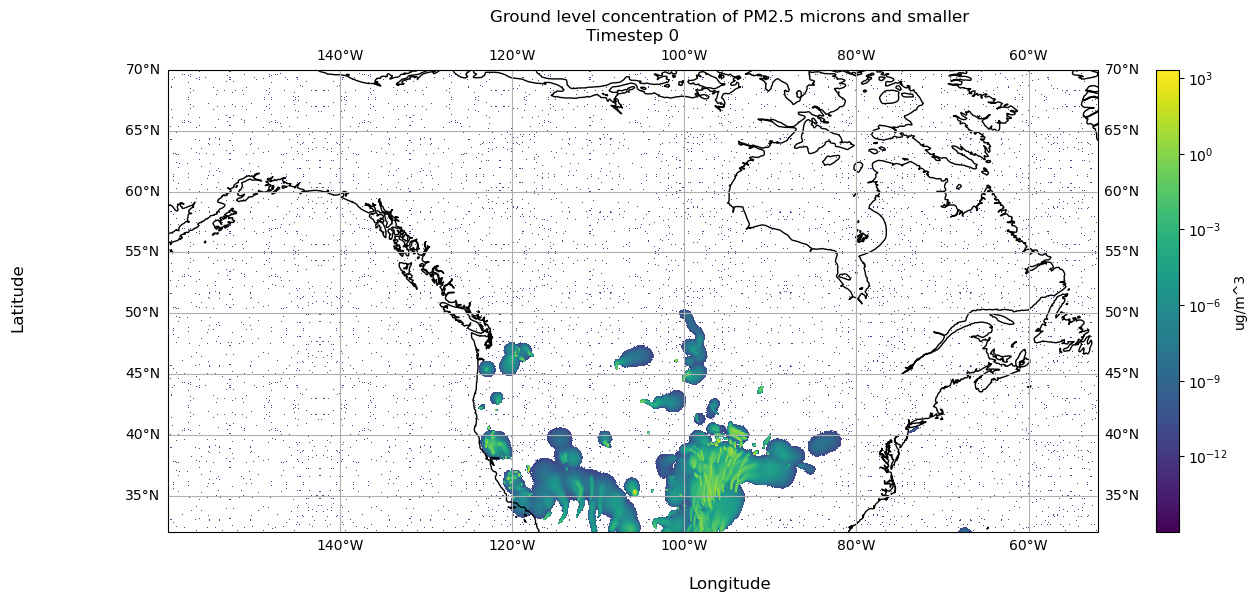
\includegraphics{data_conversion_files/figure-latex/data_notebooks-data_conversion-resample_example-cell-9-output-1.png}

\subsection{Rationale and Future
Improvements}\label{rationale-and-future-improvements-2}

\subsubsection{Discovering Varying
Grids}\label{discovering-varying-grids}

We discovered the two grid shapes in version 1 of our conversion script.
We found this after noticing the smoke data visualizations were
nonsensical.

For example, the visualizations showed smoke eminating from the ocean,
as shown in Figure~\ref{fig-resampling}.

\begin{figure}

\begin{minipage}{\linewidth}

\centering{

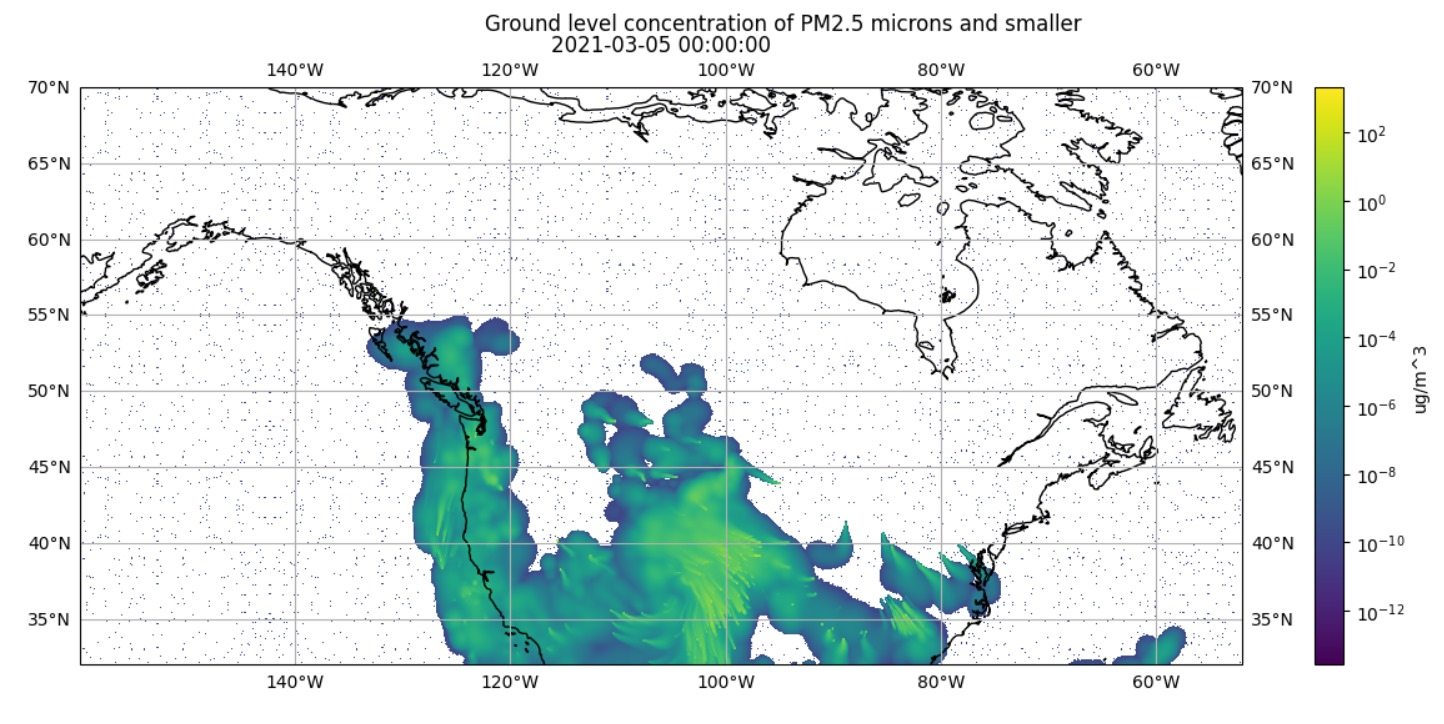
\includegraphics{images/small-on-big.jpeg}

}

\subcaption{\label{fig-small-on-big}Plotting Data from 381×1041 Grid on
381×1081 Grid}

\end{minipage}%
\newline
\begin{minipage}{\linewidth}

\centering{

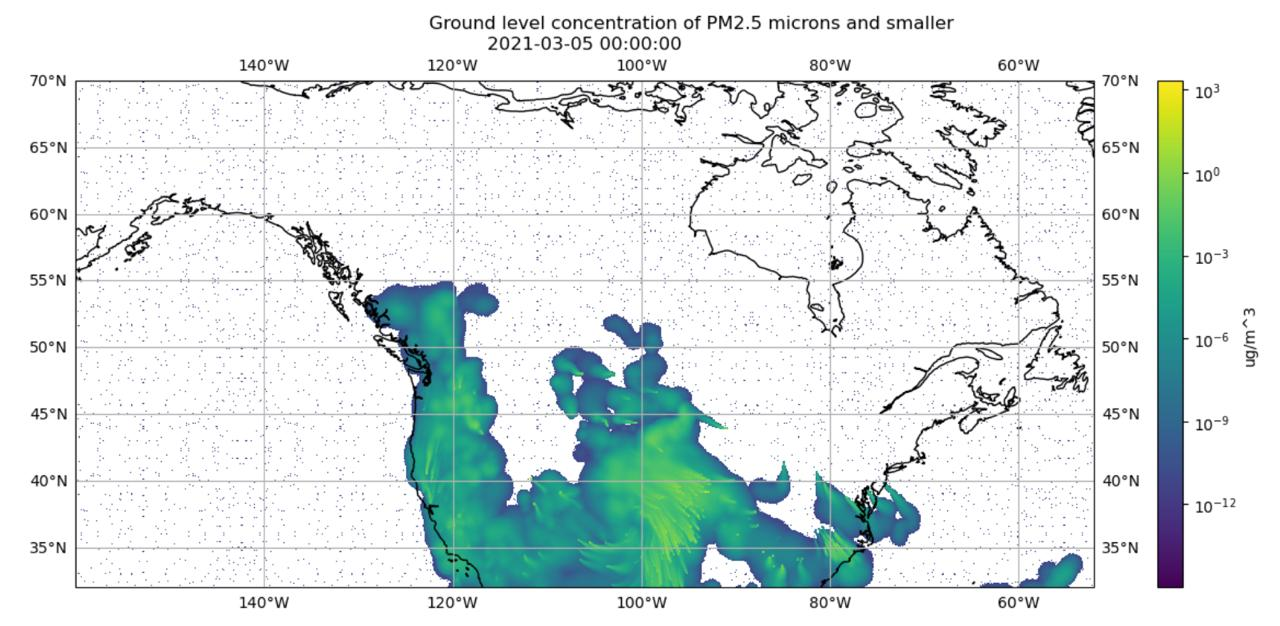
\includegraphics{images/resamped-on-big.jpeg}

}

\subcaption{\label{fig-resamped-on-big}Plotting Data Resampled from
381×1041 Grid onto 381×1081 Grid}

\end{minipage}%

\caption{\label{fig-resampling}Visualization of Timestamp March 5, 2021
00:00:00 using IDX file Created in Conversion Script Version 1}

\end{figure}%

For further details on how we investigated this issue, see
Chapter~\ref{sec-data-validation}.

\subsubsection{Handling Various Grids}\label{handling-various-grids}

We considered various approaches to handling the fact that the data was
on a 381×1041 grid or 381×1081 grid.

\begin{longtable}[]{@{}
  >{\raggedright\arraybackslash}p{(\columnwidth - 2\tabcolsep) * \real{0.3983}}
  >{\raggedright\arraybackslash}p{(\columnwidth - 2\tabcolsep) * \real{0.6017}}@{}}
\caption{The Weaknesses of Approaches to Handling Varying Array
Sizes}\label{tbl-sizes}\tabularnewline
\toprule\noalign{}
\begin{minipage}[b]{\linewidth}\raggedright
Approach
\end{minipage} & \begin{minipage}[b]{\linewidth}\raggedright
Weakness
\end{minipage} \\
\midrule\noalign{}
\endfirsthead
\toprule\noalign{}
\begin{minipage}[b]{\linewidth}\raggedright
Approach
\end{minipage} & \begin{minipage}[b]{\linewidth}\raggedright
Weakness
\end{minipage} \\
\midrule\noalign{}
\endhead
\bottomrule\noalign{}
\endlastfoot
Exclude arrays with 1041 columns. & Throwing away those data points
would discard all the information they hold. \\
Force data with 1041 columns into an array with 1081 columns without
resampling. & This results in unused columns within the 1081-column
array, leading to discontinuities and potential artifacts in the data
representation. \\
Crop arrays on 1081 columns to 1041 columns & Cropping the data would
result in loss of information. \\
\end{longtable}

The approach we chose was to \textbf{resample the data with 1041 columns
to arrays with 1081 columns}. This produced the most visually appealing
result and preserved the most information possible.

\subsubsection{Scaling}\label{scaling}

One future improvement is to generalize precomputing additional grids if
in the future the smoke forecasts change their grid size again. As of
now we manually compute points for the 2 grid sizes.

\section{Sequencing of NetCDF Files}\label{sec-sequencing}

At this point we have the lists of openable files and our resampling
grids. Now we will determine which files to use and in what order.

\subsection{Understanding Staggered
Forecasts}\label{understanding-staggered-forecasts}

The unique challenge of UBC's short term dataset is that the forecasts
overlap, creating staggered predictions.

Let's explore these staggered forecasts to understand, how to select the
optimal predictions to create a single dataset consisting of the most
optimal predictions. For details on each forecast's time information,
please see Chapter~\ref{sec-data-source}.

Across all the NetCDF files we have downloaded, recall for every hour
there exists 1-4 different forecasts to represent that hour. We aim to
choose the forecast which best represents each hour. In order to
understand the best representation for each hour, we need to know what
hours are represented in each forecast.

\subsection{Finding Hours per Forecast
ID}\label{finding-hours-per-forecast-id}

Recall that within each set of Forecast ID files, some files failed to
download or otherwise open. Therefore, we must check exactly what set of
hours are available in each collection of forecast ID NetCDF files.

In order to make loading an hour from a specified forecast ID dataset as
easy as possible, we create a dictionary for each forecast ID set. Below
you can see the first few entries of this dictionary:

\begin{Shaded}
\begin{Highlighting}[]
\CommentTok{\#TODO}
\end{Highlighting}
\end{Shaded}

To generate this dictionary, we did the following:

\phantomsection\label{annotated-cell-17}%
\begin{Shaded}
\begin{Highlighting}[]
\NormalTok{id\_sets }\OperatorTok{=}\NormalTok{ \{id\_: \{\} }\ControlFlowTok{for}\NormalTok{ id\_ }\KeywordTok{in}\NormalTok{ ids\} }\hspace*{\fill}\NormalTok{\circled{1}}

\ControlFlowTok{for}\NormalTok{ id\_ }\KeywordTok{in}\NormalTok{ ids:}
    \CommentTok{\# get successful files to add all successful hours to set}
    \ControlFlowTok{for} \BuiltInTok{file} \KeywordTok{in}\NormalTok{ tqdm(successful\_files[id\_]): }\hspace*{\fill}\NormalTok{\circled{2}}
\NormalTok{        path }\OperatorTok{=} \SpecialStringTok{f\textquotesingle{}}\SpecialCharTok{\{}\NormalTok{firesmoke\_dir}\SpecialCharTok{\}}\SpecialStringTok{/}\SpecialCharTok{\{}\NormalTok{id\_}\SpecialCharTok{\}}\SpecialStringTok{/}\SpecialCharTok{\{}\BuiltInTok{file}\SpecialCharTok{\}}\SpecialStringTok{\textquotesingle{}} \hspace*{\fill}\NormalTok{\circled{3}}
        
\NormalTok{        ds }\OperatorTok{=}\NormalTok{ xr.open\_dataset(path) }

        \ControlFlowTok{for}\NormalTok{ h }\KeywordTok{in} \BuiltInTok{range}\NormalTok{(ds.sizes[}\StringTok{"TSTEP"}\NormalTok{]): }\hspace*{\fill}\NormalTok{\circled{4}}
\NormalTok{            id\_sets[id\_][(}\BuiltInTok{file}\NormalTok{, parse\_tflag(ds[}\StringTok{\textquotesingle{}TFLAG\textquotesingle{}}\NormalTok{].values[h][}\DecValTok{0}\NormalTok{]))] }\OperatorTok{=}\NormalTok{ h }
\end{Highlighting}
\end{Shaded}

\begin{description}
\tightlist
\item[\circled{1}]
Initialize a dictionary to hold an empty dictionary for each forecast
ID.
\item[\circled{2}]
We step through all the successfully opened files found for
\texttt{id\_}.
\item[\circled{3}]
Open the file and open it using \texttt{xarray}.
\item[\circled{4}]
Create a tuple with the file name and the parsed TFLAG for current hour
\texttt{h}. Add index \texttt{h} to our dictionary assigning the tuple
as its key.
\end{description}

\subsection{Creating the Sequence}\label{creating-the-sequence}

Now that we have an indexable set of all available hours for each
forecast ID, we can generate the sequence to extract the time series
dataset we would like to create.

\section{Creating the IDX File}\label{creating-the-idx-file}

At this point, we have precomputed the order in which we will load and
write each array to our IDX file. We will now put everything together to
generate our single dataset.

\phantomsection\label{annotated-cell-18}%
\begin{Shaded}
\begin{Highlighting}[]
\NormalTok{f }\OperatorTok{=}\NormalTok{ Field(}\StringTok{"PM25"}\NormalTok{, }\StringTok{"float32"}\NormalTok{) }\hspace*{\fill}\NormalTok{\circled{1}}

\NormalTok{db }\OperatorTok{=}\NormalTok{ CreateIdx( }\hspace*{\fill}\NormalTok{\circled{2}}
\NormalTok{    url}\OperatorTok{=}\NormalTok{idx\_dir }\OperatorTok{+} \StringTok{"/firesmoke.idx"}\NormalTok{,}
\NormalTok{    fields}\OperatorTok{=}\NormalTok{[f],}
\NormalTok{    dims}\OperatorTok{=}\NormalTok{[}\BuiltInTok{int}\NormalTok{(max\_ncols[ids[}\DecValTok{0}\NormalTok{]]), }\BuiltInTok{int}\NormalTok{(max\_nrows[ids[}\DecValTok{0}\NormalTok{]])],}
\NormalTok{    time}\OperatorTok{=}\NormalTok{[}\DecValTok{0}\NormalTok{, }\BuiltInTok{len}\NormalTok{(idx\_calls) }\OperatorTok{{-}} \DecValTok{1}\NormalTok{, }\StringTok{"\%00000000d/"}\NormalTok{],}
\NormalTok{) }

\NormalTok{tstep }\OperatorTok{=} \DecValTok{0} \hspace*{\fill}\NormalTok{\circled{3}}

\NormalTok{thresh }\OperatorTok{=} \FloatTok{1e{-}15} \hspace*{\fill}\NormalTok{\circled{4}}

\ControlFlowTok{for}\NormalTok{ call }\KeywordTok{in}\NormalTok{ tqdm(idx\_calls): }\hspace*{\fill}\NormalTok{\circled{5}}
\NormalTok{    curr\_id }\OperatorTok{=}\NormalTok{ call[}\DecValTok{0}\NormalTok{]}
\NormalTok{    curr\_file }\OperatorTok{=}\NormalTok{ call[}\DecValTok{1}\NormalTok{]}
\NormalTok{    tstep\_index }\OperatorTok{=}\NormalTok{ call[}\DecValTok{3}\NormalTok{] }

\NormalTok{    ds }\OperatorTok{=}\NormalTok{ xr.open\_dataset(}\SpecialStringTok{f"}\SpecialCharTok{\{}\NormalTok{firesmoke\_dir}\SpecialCharTok{\}}\SpecialStringTok{/}\SpecialCharTok{\{}\NormalTok{curr\_id}\SpecialCharTok{\}}\SpecialStringTok{/}\SpecialCharTok{\{}\NormalTok{curr\_file}\SpecialCharTok{\}}\SpecialStringTok{"}\NormalTok{) }\hspace*{\fill}\NormalTok{\circled{6}}

\NormalTok{    file\_vals }\OperatorTok{=}\NormalTok{ np.squeeze(ds[}\StringTok{"PM25"}\NormalTok{].values) }\hspace*{\fill}\NormalTok{\circled{7}}

\NormalTok{    resamp }\OperatorTok{=}\NormalTok{ ds.XORIG }\OperatorTok{!=}\NormalTok{ max\_xorig }\hspace*{\fill}\NormalTok{\circled{8}}

    \ControlFlowTok{if}\NormalTok{ resamp: }\hspace*{\fill}\NormalTok{\circled{9}}
\NormalTok{        file\_vals\_resamp }\OperatorTok{=}\NormalTok{ griddata(}
\NormalTok{            sml\_tups,}
\NormalTok{            file\_vals[tstep\_index].flatten(),}
\NormalTok{            big\_tups,}
\NormalTok{            method}\OperatorTok{=}\StringTok{"cubic"}\NormalTok{,}
\NormalTok{            fill\_value}\OperatorTok{=}\DecValTok{0}\NormalTok{,}
\NormalTok{        ) }

\NormalTok{        file\_vals\_resamp[file\_vals\_resamp }\OperatorTok{\textless{}}\NormalTok{ thresh] }\OperatorTok{=} \DecValTok{0} \hspace*{\fill}\NormalTok{\circled{10}}

\NormalTok{        file\_vals\_resamp }\OperatorTok{=}\NormalTok{ file\_vals\_resamp.reshape((}\BuiltInTok{len}\NormalTok{(big\_lat), }\BuiltInTok{len}\NormalTok{(big\_lon))) }\hspace*{\fill}\NormalTok{\circled{11}}

\NormalTok{        db.write(data}\OperatorTok{=}\NormalTok{file\_vals\_resamp.astype(np.float32), field}\OperatorTok{=}\NormalTok{f, time}\OperatorTok{=}\NormalTok{tstep) }\hspace*{\fill}\NormalTok{\circled{12}}
    \ControlFlowTok{else}\NormalTok{: }\hspace*{\fill}\NormalTok{\circled{13}}
\NormalTok{        db.write(data}\OperatorTok{=}\NormalTok{file\_vals[tstep\_index], field}\OperatorTok{=}\NormalTok{f, time}\OperatorTok{=}\NormalTok{tstep) }

\NormalTok{    tstep }\OperatorTok{=}\NormalTok{ tstep }\OperatorTok{+} \DecValTok{1} \hspace*{\fill}\NormalTok{\circled{14}}
\end{Highlighting}
\end{Shaded}

\begin{description}
\tightlist
\item[\circled{1}]
Create an OpenVisus field to hold the PM25 variable data.
\item[\circled{2}]
Create the IDX file wherein \texttt{url} is the location to write the
file, \texttt{fields} holds the data variables we will save,
\texttt{dims} represents the shape of each array, and \texttt{time}
defines how many time steps there are.
\item[\circled{3}]
We will usethis to keep track of which time step we are on as we step
through our \texttt{idx\_calls}.
\item[\circled{4}]
Threshold to use to change small-enough resampled values to 0.
\item[\circled{5}]
Get the information for current time step, in particular the
{[}curr\_id, file\_str,
parse\_tflag(ds{[}`TFLAG'{]}.values{[}tstep\_idx{]}{[}0{]}),
tstep\_idx{]}
\item[\circled{6}]
Load the current file with \texttt{xarray}.
\item[\circled{7}]
Get the full array of PM25 values in the file.
\item[\circled{8}]
If \texttt{ds.XORIG} is not already for the 381×1081 grid, we need to
resample it to the larger grid.
\item[\circled{9}]
Using \texttt{gridddata}, interpolate the values on a 381×1081 grid
using the precomputed lat/lon points.
\item[\circled{10}]
Any values that are less than our threshold should have a value of 0.
WHY
\item[\circled{11}]
Reshape the interpolated values to 381×1081.
\item[\circled{12}]
Write the resampled values for hour \texttt{h} to timestep \texttt{t}
and field \texttt{f} of our IDX file.
\item[\circled{13}]
These values are already on a 381×1081 grid, so write the values at hour
\texttt{h} to timestep \texttt{t} and field \texttt{f} of our IDX file.
\item[\circled{14}]
Increment to the next timestep for writing to IDX.
\end{description}

\bookmarksetup{startatroot}

\chapter{Data Validation}\label{sec-data-validation}

The success of this data curation project requires compotent data
validation. Data validation is the bridge between theoretical and
real-world data curation. We unfortunately used many assumptions about
the data and systems we used that did not hold true, leading to
unexplainable issues throughout the data curation process.

Here, we will describe our deficiencies in performing data validation
and the consequences we faced. We conclude with a discussion on how best
data validation can be incorporated in this project and future such
projects, so that one may avoid such issues next time.

\section{Data Validation vs Data
Exploration}\label{data-validation-vs-data-exploration}

Data exploration enlightens one on the contents of the data and metadata
one presumes they have. We performed data exploration by loading and
visualizing a few files. This allowed us to understand what data UBC
aims to provide.

What data exploration \emph{does not} do is explain the origin of issues
such missing or seemingly corrupt data. Data exploration uses the
assumption that the data is perfect.

Data validation forces one to consider, where do issues that appear in
the data come from, and are these issues with the data or with the
systems used to access and manipulate the data?

\section{Data Loading}\label{data-loading}

Most of the issues we faced during data curation resulted from failing
to validate our data loading system.

\section{Data Conversion}\label{data-conversion}

\bookmarksetup{startatroot}

\chapter*{References}\label{references-2}
\addcontentsline{toc}{chapter}{References}

\markboth{References}{References}

\phantomsection\label{refs}
\begin{CSLReferences}{0}{1}
firesmoke.ca

\end{CSLReferences}




\end{document}
